\documentclass{article}
\usepackage{geometry}
\geometry{a4paper, 
margin=1in}
\usepackage{longtable}
\usepackage{amsmath}
\usepackage{amssymb}
\usepackage{booktabs}
\usepackage{xcolor}
\usepackage{hyperref}
\usepackage{graphicx} % Required for including images
\usepackage{subcaption}  % Required for subfigures
\usepackage{tcolorbox}  % For colored boxes
% \geometry{margin=1in}
\usepackage{booktabs}    % \toprule, \midrule, \bottomrule
\usepackage{caption}     % if you need \caption* or extra caption control
\usepackage{longtable}   % if your table might span multiple pages
\usepackage{array}       % for more flexible column specs (e.g. >{\ttfamily}l)
\usepackage{multirow}
\usepackage{tabularx}
\usepackage{array}
\usepackage{multirow}
\usepackage{booktabs}

% \title{Zoobenthic Community Indicators of Sediment Contamination}

% \author{Feng Gu}

\begin{document}
% \maketitle

\begin{titlepage}
\centering
\vspace*{2cm}

{\LARGE\bfseries Zoobenthic Community Indicators of Sediment Contamination\par}
\vspace{1.2cm}

{\Large\textbf{Research Proposal}\par}
\vspace{1.5cm}

{\large\textbf{Author:} Feng Gu\par}
\vspace{0.5cm}

{\large\textbf{Program and Institution:}\par}
\vspace*{.2cm}
{\large Master of Science (M.Sc.) in Data Science\\
\vspace*{.2cm}
Thompson Rivers University (TRU), Kamloops, British Columbia, Canada\par}
\vspace{1.5cm}

{\Large\textbf{Supervisory Committee:}\par}
\vspace*{.2cm}
{\large
Dr. Jabed H. Tomal (Supervisor) — Department of Mathematics and Statistics, TRU\\
\vspace*{.2cm}
Dr. Yue Zhang (Co-supervisor) — Department of Mathematics and Statistics, TRU\\
\vspace*{.2cm}
Prof. Jan Ciborowski (Committee Member) — Department of Biological Sciences, University of Calgary
\par}

\vfill
{\large October 2025\par}

\end{titlepage}


\clearpage

\begin{center}
    {\Large \textbf{Abstract}}
\end{center}

This proposal reviews the rationale and analytical framework of Zoobenthic Community Indicators (ZCI)
of Sediment Contamination in aquatic ecosystems. 
Building upon this foundation, the author outlines the research objectives and discusses
the key methodologies to be applied.
Preliminary results are produced based on the framework described in the \textit{Methodology} section,
demonstrating the feasibility of the proposed approach 
and supporting the achievability and significance of the research objectives.  

This proposal comprises eight main sections. 
The \textbf{Introduction} presents the research topic, describes the general relationships among its fundamental components and 
introduces the study system. 
The \textbf{Research Objectives} section defines the specific goals and principal questions to be addressed in the project. 
The \textbf{Data Description} outlines the dataset characteristics, including data types, sources, collection methods, and variable definitions. 
The \textbf{Literature Review} synthesizes relevant research on the close study objectives and their analytical approaches.
The \textbf{Methodology} section presents the overall analytical framework and discusses specific techniques, with several figures provided 
to illustrate the idealized workflow. 
The \textbf{Preliminary Results} section reports initial outcomes from implementing key methodological steps, demonstrating both 
the feasibility and scalability of the proposed framework. 
The \textbf{Practical Implementation Plan} describes the computational strategies supporting the research objectives, including 
the structure of the codebase and choice of programming languages. 
The \textbf{Supervisory Dissolution} section summarizes supervision conditions and acknowledgements, 
and the \textbf{Timeline} outlines a provisional schedule with major milestones for completion of each research phase.  


\clearpage
\tableofcontents

\clearpage
\newcommand{\noticingbox}[2]{
    \begin{tcolorbox}[colback=yellow!10!white,
                                        colframe=orange!90!black,
                                        title = #2,
                                        fonttitle=\bfseries]
        #1
    \end{tcolorbox}
}

\newcommand{\refcolor}[1]{\textcolor{blue}{\ref{#1}}
} % Custom commands for convenience
\section{Introduction}

% \textcolor{blue}{(Background about the study area)}

\subsection{Sediment contamination in aquatic ecosystems}
% great lakes are important

Rivers and lakes provide essential services for human well-being and biodiversity \cite{Vörösmarty2010GlobalThreats}.
% sediments store many nutrients and contaminants
With intensive industrial and urban development along the shorelines, anthropogenic activities have released 
significant amount of pollutants into the these aquatic ecosystems \cite{DavidAllan2013},
elevating ecological risks as many of these contaminants bioaccumulate in aquatic organisms and eventually enter human 
food chains through fish consumption, posing health risks \cite{Eggleton2004SedDisturbance, USGS_SedimentAssociatedContaminants_2019}.
These ecological and human health risks underscore the urgent need for scientific assessment to inform management strategies \cite{Niemi2004EcologicalIndicators}.

Most of these anthropogenic inputs enter the water through 
both point and non-point sources, carrying two major groups of components: 
nutrients (which are water soluble) and hydrophobic contaminants \cite{Carpenter1998Nonpoint}.
The nutrients (especially phosphorus) are taken up by algae, contributing to eutrophication.
However, hydrophobic chemicals
quickly attach to floating organic particles and settle into the muddy bottom sediments through natural binding processes \cite{DavidAllan2013}.
There they accumulate at the bottom where water meets sediment.
Similar binding and absorption processes turn bottom sediments into
a combined storage area of past pollution \cite{Eggleton2004SedDisturbance, USGS_SedimentAssociatedContaminants_2019, ChiaiaHernandez2022,Burton2002SedQuality}.
The chemicals bounded to sediment particles remain chemically stable for extended periods, effectively preserving pollutant signatures 
and creating a persistent record of contamination events across multiple temporal scales \cite{ChiaiaHernandez2022, Burton2002SedQuality}.
This integrative role establishes sediments as a biogeochemical archive that smooths short-term water column fluctuations,
making sediment contaminant measurements a robust long-term {manifestation} of anthropogenic stress \cite{Karickhoff1984Sorption}.


\subsection{Benthic communities as bioindicators for sediment contamination}
Analysis of the chemical content of sediment is resource-intensive and overlooks bioavailability
(the likelihood that chemicals are transferred to biota),
necessitating complementary indicator approaches \cite{Chapman1990SedimentTriad}.
In most natural ecosystems, individual organisms exhibit physiological and behavioral adjustments under external pressures; 
aquatic benthic macroinvertebrates likewise express stressor-mediated responses that scale to detectable community change \cite{Holling1973}.
Benthic macroinvertebrate assemblages can reflect concentrations of sediment-borne contaminants and habitat conditions \cite{Tampo2021Bioindicators},
rendering them effective bioindicators of sediment contamination levels \cite{Desrosiers2020}.
These responses can be observed through differences in benthic community composition and many attempts to develop indices on small aquatic systems, 
such as small lakes, rivers, and streams, have been shown successful \cite{Cain1992Bioindicators, Archaimbault2010SedimentStreams},
motivating extension to large lakes and great rivers where fewer attempts were made but are promising
 by some successful implementations \cite{Birk2012Methods,Ciborowski2005ZoobenthicIndicators, Reynoldson1995}.

Effective bioindicator development requires balancing ecological relevance with practical applicability.
Ideal taxa should exhibit sensitivity to pollution gradients, maintain wide distribution across environmental gradients within the study area,
and be readily sampled and taxonomically identified \cite{LenatResh2001Taxonomy}.
In large aquatic ecosystems, environmental complexity and heterogeneity present additional challenges for bioindicator development,
necessitating the inclusion of diverse taxa assemblages that influence both indicator construction and interpretation \cite{Menezes2010Trait, Bonada2006BiomonitoringReview}.
Through strategic selection of an appropriate taxonomic pool, it becomes feasible to develop robust and sensitive bioindicators 
for sediment contamination assessment \cite{LenatResh2001Taxonomy}.


\subsection{Variation in community composition across environmental gradients}

Zoobenthic communities vary with respect to both anthropogenic stressors (e.g., sediment contaminants) 
and natural environmental variability (e.g., substrate, temperature, flow) \cite{PasanenMortensen2013FoxLynx}.
Under consistent environmental conditions, community composition prior to anthropogenic influence 
represents the naturally-shaped baseline for comparison following pollution onset \cite{Reynoldson1997ReferenceCondition}.

In pervasively human-influenced regions, zoobenthic community composition is obscured by the combined influence of
anthropogenic stressors and natural environmental variability \cite{Stoddard2006}.
This necessitates identifying and isolating the pre-pollution community composition from observed levels,
since only the anthropogenically-driven component is relevant for developing
bioindicators of sediment contamination \cite{Reynoldson1997ReferenceCondition}.

Therefore, partitioning community composition into naturally-driven and pollution-driven components 
is essential for sediment contamination bioindicator development \cite{Reynoldson1997ReferenceCondition}.
The natural component provides the taxonomic baseline and enables quantification of anthropogenic deviations,
thereby isolating the pollution-driven signal across temporal scales
for indicator construction \cite{Legendre2008VariationPartitioning}.

Building upon this environmental context, these three components - 
benthic communities, sediment contamination, and natural environmental gradients 
- interact and reveal zoobenthic community responses to external changes.
Figure \textcolor{blue}{\ref{fig:introduction_study_system}} provides a conceptual overview 
of how zoobenthic communities exist within this context,
illustrating the framework for understanding community responses to anthropogenic stressors.


\subsection{Accounting for spatial structure and autocorrelation}
Spatial location and local environmental attributes (i.e., ecological covariates) of sampling sites represents easily collected yet frequently overlooked information.
Many studies assume that zoobenthic communities are shaped identically by natural attributes
irrespective of their spatial positions \cite{Borcard1992SpatialPartialling},
bringing simplicity in quantitative analysis but this may not hold in all real scenarios.

Advances in spatial statistics and computational power now enable incorporation of ecosystem spatial structure 
and linking environmental complexity to geo-heterogeneity \cite{Borcard2002PCNM,Harris2011GWPCA}.
Accumulating studies demonstrate that natural heterogeneity is spatially structured
across ecosystems and that modeling this structure substantially improves explanation for community variation \cite{Turner1989PatternProcess,Borcard1992SpatialPartialling,Borcard2002PCNM}.
The primary rationale is that many unmeasured or unmeasurable natural environmental attributes have their own spatial signatures,
enabling spatial variables to serve as proxies for these hidden drivers \footnote{
This approach parallels the use of instrumental variables and proxy variables in econometrics, 
where measurable variables are employed to control for unmeasured confounders and enable causal inference. 
} \cite{Dormann2007SpatialAutocorrelation,Turner1989PatternProcess}.
Therefore, incorporating essential spatial analysis is a promising method to
control more natural variation in community composition,
ultimately bringing a clearer picture of zoobenthic community responses
to sediment contamination \cite{Legendre2008VariationPartitioning}.

\subsection{Study system: St. Clair-Detroit River System}

These mechanistic principles provide the theoretical foundation for developing a
bioindicator of sediment contamination that controls for environmental and spatial variability.
To implement this framework, this study will apply quantitative methods
within the St. Clair-Detroit River System (SCDRS) of the Great Lakes.

As one of the world's largest surface freshwater ecosystems, 
the Great Lakes region contains 21\% of the global supply of surface fresh water 
and supports the livelihoods of millions of people \cite{EPA_Greatlakes2024}.
While much of the Great Lakes region remains minimally disturbed,
certain areas have historically suffered from intensive anthropogenic activities \cite{EPA_SOGL2007}.
These heavily impacted areas are primarily concentrated along western Lake Erie's shorelines and its connecting waterways,
particularly the Detroit River\cite{EPA_SOGL2007, Drouillard2006, Ciborowski1988}, making these regions intensively monitored and studied.

Leveraging available data compiled and integrated by Zhang \cite{Zhang2008} with other sources
(Farara and Burt 1993 \cite{Farara1993}; Wood 2004 \cite{Wood2004}), this study
will use dataset from the Huron-Erie corridor that comprises the St. Clair-Detroit River System (SCDRS).
This corridor forms a connected water system
characterized by areas of fast flow where the channel is constricted
\footnote{
Channel constriction occurs when water flow is forced through a narrower cross-sectional area,
resulting in increased velocity and turbulence according to the continuity 
equation in fluid dynamics.} and by extensive anthropogenic pollution from
upstream sources and bordering shorelines.
Among the three segments, the Detroit River will be the primary focus due to its intensive human influence
and the availability of extensive benthic community and sediment contamination data (\cite{Zhang2008}).
By developing this bioindicator framework on the surveyed area, this case study is expected 
to advance bioindicator research applicable to other large lakes and rivers and to 
provide a methodological foundation for broader application across the Great Lakes region.

\begin{figure}[!h]
    \centering
    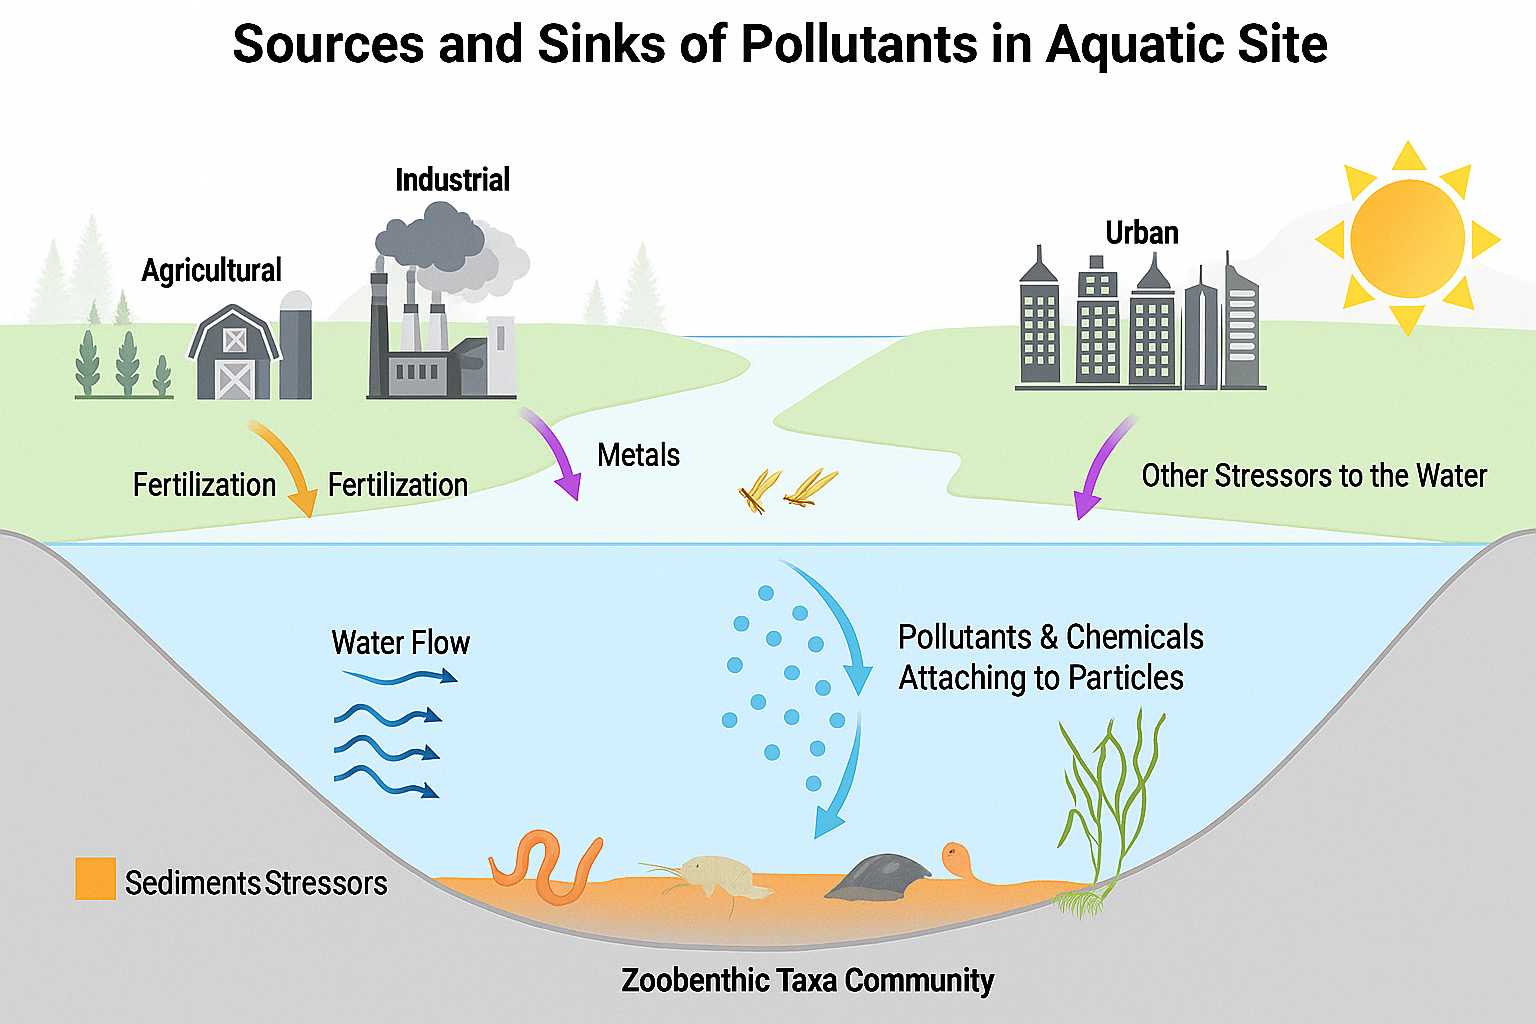
\includegraphics[width=0.9\textwidth]{../results/ideas_visualization/introduction_study_system.png}
    \caption{\textit{Overview of how zoobenthic communities live under both sediment contamination and natural environmental conditions, 
    and may respond to these external changes. 
    (Base template adapted from Selvi \textit{et al.} (2019) \cite{Selvi2019}, originally created and shared on \textbf{BioRender}. 
    Modified by Feng Gu using \textbf{Sora2} with text-based prompts.)}}
    \label{fig:introduction_study_system}

\end{figure}
\clearpage
\section{Research Objectives}

The goal of this study is to build a zoobenthic community indicator(ZCI) of sediment contamination 
in a large aquatic ecosystem(e.g., SCDRS or Detroit River) by means of multivariate statistical analysis.
This work can be divided into five specific objectives with respects to aquatic ecology principles and
statistical methodologies:

\begin{enumerate}
    \item Build quantitative composite measures of sediment contamination levels and zoobenthic community composition.
        \item Control for natural variability in community composition and isolate anthropogenic effects on community composition.
        \item Incorporate spatial features to account for potential spatial heterogeneity in community composition.
        \item Model the relationship between the sediment contamination levels and zoobenthic community composition
        with piecewise quantile regression and extend it to a bioindicator (ZCI) of sediment contamination level.
        \item Evaluate the indicator power and robustness of the developed ZCI with respect
        to sample size and other relevant global factors that can influence the estimates.
\end{enumerate}

These listed objectives are made in a tentatively sequential order. Some objectives have been well-supported by
existing researches while others are more exploratory. Objectives \textcolor{blue}{1, 2} and \textcolor{blue}{4},
form a good benchmark of building the zoobenthic community indicator and are supported by a well-established
\textbf{Multivariate Community Indicator Framework}
\footnote{Its details are provided in following content and in the Methodology section}
\cite{Brazner2007, Kovalenko2014, Host2019, Ciborowski2005ZoobenthicIndicators,Zhang2008}
amenable to application of a piecewise quantile regression model.
Objectives \textcolor{blue}{3} and \textcolor{blue}{5} require exploratory investigations, 
and will serve to enhance and increase understanding of the indicator's power and sensitivities.

The following subsections disccussed the proposed general approach, highlighting the focuses where possible contributions
can be made.

\subsection{Multivariate community indicator framework}

Multivariate community indicator framework is a comprehensive approach for achieving objectives \textcolor{blue}{1, 2} and \textcolor{blue}{4}, 
we will build it with possible improvements.
Three data matrices (Zhang 2008 \cite{Zhang2008}; Farara and Burt 1993 \cite{Farara1993}; Wood 2004 \cite{Wood2004}) will be used for it:
the taxa matrix (biological response), the environmental covariate matrix, and the stressor (chemical) matrix.
Furthermore, quantitative indices that summarize sediment contamination and zoobenthic community composition
will be designed and applied meanwhile controlling the natural variability. 
Its basic steps are summarized as follows:

\begin{enumerate}
    \item \textbf{Measure sediment contamination and select reference sites}
    
    \emph{Motivation: establish a defensible composite measure that reflects a contamination gradient and identify 
    least disturbed sites that serve as reference locations.}

    Perform Principal Component Analysis (PCA) on elements of the stressor matrix;
    filter and interpret qualified pollutant Principal Components (PCs) from which to form a
    composite contamination score. Designate sites with the scores indicative of minimally-disturbed
    levels as reference sites from which to identify their putative "reference condition" assemblages.

    \item \textbf{Predict 'reference condition' community composition across environmental gradients} 
    
    \emph{Motivation: predict the variation in community composition as controlled by environmental covariates
    to disentangle the pollution-driven deviation in the community composition.}

    Perform hierarchical agglomerative cluster analysis of the biota of reference-site samples to identify
    distinct groups of taxa; train a discriminant model to predict the biological assemblages present at 
    a location on the basis of the location’s environmental conditions. 
    Thus, sites having the same biological assemblage are considered environmentally homogeneous.

    \item \textbf{Measure community composition (ZCI) for environmentally homogeneous sites}

    \emph{Motivation: construct a numerical index for each biological assemblage to summarize
    community composition for sites with similar environmental conditions.}

    Within each predicted cluster, apply ordination (e.g., PCA/NMDS) to summarize taxa information;
    derive the measurement results as ZCI with defined scoring rules.
    Sites deviating from the reference site centroid are considered disturbed by pollution,
    they compromise the disturbance-relevant ZCI results.

    \item \textbf{Quantify the relationship between contamination level and ZCI}
    
    \emph{Motivation: quantify how community composition responds to contamination levels}

    Fit regression models of ZCI deviation versus contamination score to capture deterministic relationships 
        and stochastic variation that shapes the conditional distributional response.
        Determining a suitable relationship pattern, e.g., smooth linear or breakpoint-based piecewise,
        is the key to the first step.
        If the latter exists, the following tasks will be to identify (1) the level of contamination at which the breakpoint(s) occur and
        (2) the benchmark(s) of ZCI representative of these crucial contamination levels.
\end{enumerate}



\subsection{Spatial heterogeneity test and incorporation}

Objective \textcolor{blue}{3} is to ensure the unmodelled spatial patterns do not confound the regression results.
Ecological data often exhibit spatial autocorrelation—nearby sites tend to have similar communities—so
failing to include spatial structure can lead to biased estimates and inflated error rates.
The principal coordinates of neighbour matrices (PCNM) method will be applied to transform spatial distances among sites into orthogonal spatial
predictors that can be incorporated into regression or canonical analyses \cite{Borcard2002PCNM, Dray2006SpatialEigenfunction, GriffithPeresNeto2006SpatialFiltering}.

PCNM eigenvectors from the Euclidean distance matrix will capture spatial structure at different scales \cite{Borcard2002PCNM, GriffithPeresNeto2006SpatialFiltering}.
For each environmental cluster of sample sites, we will test for spatial heterogeneity by regressing the ZCI 
derived for that group of sites against PCNM vectors 
to identify significant spatial predictors not explained by environmental variables.
Selected PCNM variables will be incorporated as covariates in quantile regression models to control spatial autocorrelation.
% Variance partitioning will help control the correlation among contamination levels across space,
% improving the accuracy in estimating the ZCI-contamination relationship.

\subsection{Piecewise quantile regression for breakpoint in quantile relationship}

Objective~\textcolor{blue}{4} is to use a piecewise quantile regression to model the relationship 
between sediment contamination levels and a ZCI,
which identifies breakpoints in the ZCI-contamination relationship within the multivariate community indicator framework. 
Piecewise quantile regression (PQRM) is chosen for its ability to estimate conditional quantiles 
of a response without assuming a specific parametric form \cite{Cade2003,Huang2017}, 
to model the entire conditional distribution rather than just the mean \cite{Cade2003},
and to estimate parameters that are robust to outliers or heteroscedastic variance \cite{Huang2017}.
In the ecological context, quantile regression can reveal abrupt changes in zoobenthic community 
composition associated with specific contamination levels at different quantiles 
(e.g., high quantile representing sensitive taxa)
and detect breakpoints that indicate ecological thresholds \cite{Jabed2020,Spake2022,Daily2012}.

It is informative to detect threshold(s) in contamination levels across which the slope of the ZCI–contamination relationship 
changes abruptly, indicating points where benthic communities change their way in responding to contamination. 
Higher quantiles may reveal steeper changes than median quantiles, highlighting vulnerable taxa. 
Comparing breakpoints across environmentally distinct clusters (if the comparison across environmental gradients is feasible)
will show whether thresholds vary among environmental gradients.


\subsection{Indicator power and robustness with respect to sample size}
The goal of Objective~\textcolor{blue}{5} is to evaluate how reliably
the ZCI detects sediment contamination gradients under varying sampling restrictions and conditions.
Two primary targets can be (1) exploring the minimum size of training data that supports the reliable estimation 
of key parameters (e.g., slopes, breakpoints)\cite{Spake2022} in the ZCI–contamination relationship; 
(2) how large a test set should be used to determine whether a new site falls above or below 
particular threshold(s) with acceptable probabilistic confidence when it truly does so.


Robustness analyses are essential because bioindicator performance can deteriorate when sample sizes are small, variance components are poorly estimated, or site selection produces hidden pseudoreplication \cite{Hurlbert1984Pseudo}. Power and precision directly influence management credibility; underpowered indicators risk Type II errors (failing to flag degraded conditions) while unstable estimates inflate Type I error rates in threshold detection \cite{Osenberg1994ImpactPower,Fairweather1991MonitoringPower}.

The analytical approach is tentatively to use bootstrap resampling and subsampling to evaluate ZCI robustness.
Bootstrap resampling may generate sampling distributions for key parameters (slopes, breakpoints, pseudo-$R^2$),
while subsampling could construct precision curves by repeatedly selecting subsets of sites across sample sizes.
Power analysis will potentially simulate datasets under null and alternative hypotheses to compute detection power
for contamination effects and threshold shifts. Spatial autocorrelation may need to adjust effective sample sizes,
and breakpoint reliability could be assessed through confidence interval width criteria or other suitable metrics.


Results will identify optimal sampling design (sites per cluster) and provide decision-support tables
linking confidence levels to required sampling effort. Higher quantiles may require larger samples due to greater dispersion,
while also elevating the potential concerns regarding spatial autocorrelation.






\section{Data Description}

\subsection{Data Collection}

The data used in this program is provided by Dr. Ciborowski, collected and 
processed by Zhang.
It consists of data from
three separate surveys conducted in: 1991, 1999 and 2004 (Zhang \cite{Zhang2008}; Farara and Burt 1993 \cite{Farara1993}; Wood 2004 \cite{Wood2004}),
all following the same field protocols
\footnote{
These sampling locations were determined prior to 
fieldwork by a stratified random sampling design to ensure representative coverage.}.

The 2004 data set was collected by Zhang \cite{Zhang2008} and principally across the entire SCDRS zone.
The information collected includes sample location information (longitude and latitude),
16 zoobenthic taxonomic variables, 5 environmental
variables (e.g., temperature, pH, dissolved oxygen), and 30 stressors representing trace metals,
polyaromatic hydrocarbons (PAHs).
The data from two previous studies, which collected data from the Detroit River zone in 1991 and 1999
(Farara and Burt 1993 \cite{Farara1993}; Wood 2004 \cite{Wood2004})—were compiled and incorporated into the 2004 data.
This combination enhances the dataset's robustness by providing a more comprehensive perspective on
the benthic community dynamics, environmental conditions, and sediment contamination across the entire Corridor over time.


Given the temporal and spatial distribution of sampling across three survey years,
\textbf{StationID serves as the primary key for data integration and site identification.}
{Each StationID uniquely identifies a sampling site in both temporal and spatial dimensions, 
meaning observations with the same StationID represent identical location-time combinations 
from the three survey years (1991, 1999, 2004).}

\subsection{Prepare a complete sub-dataset for preliminary analysis}

Taxonomic, environmental, and stressor data for sampled sites were originally stored in three separate tabular files.
For preliminary analysis, we made a quick check on the data quality and completeness
\footnote{By the submission 
of the proposal the latest check was done on July 24, 2025.}.

\begin{figure}[!h]
    \centering
    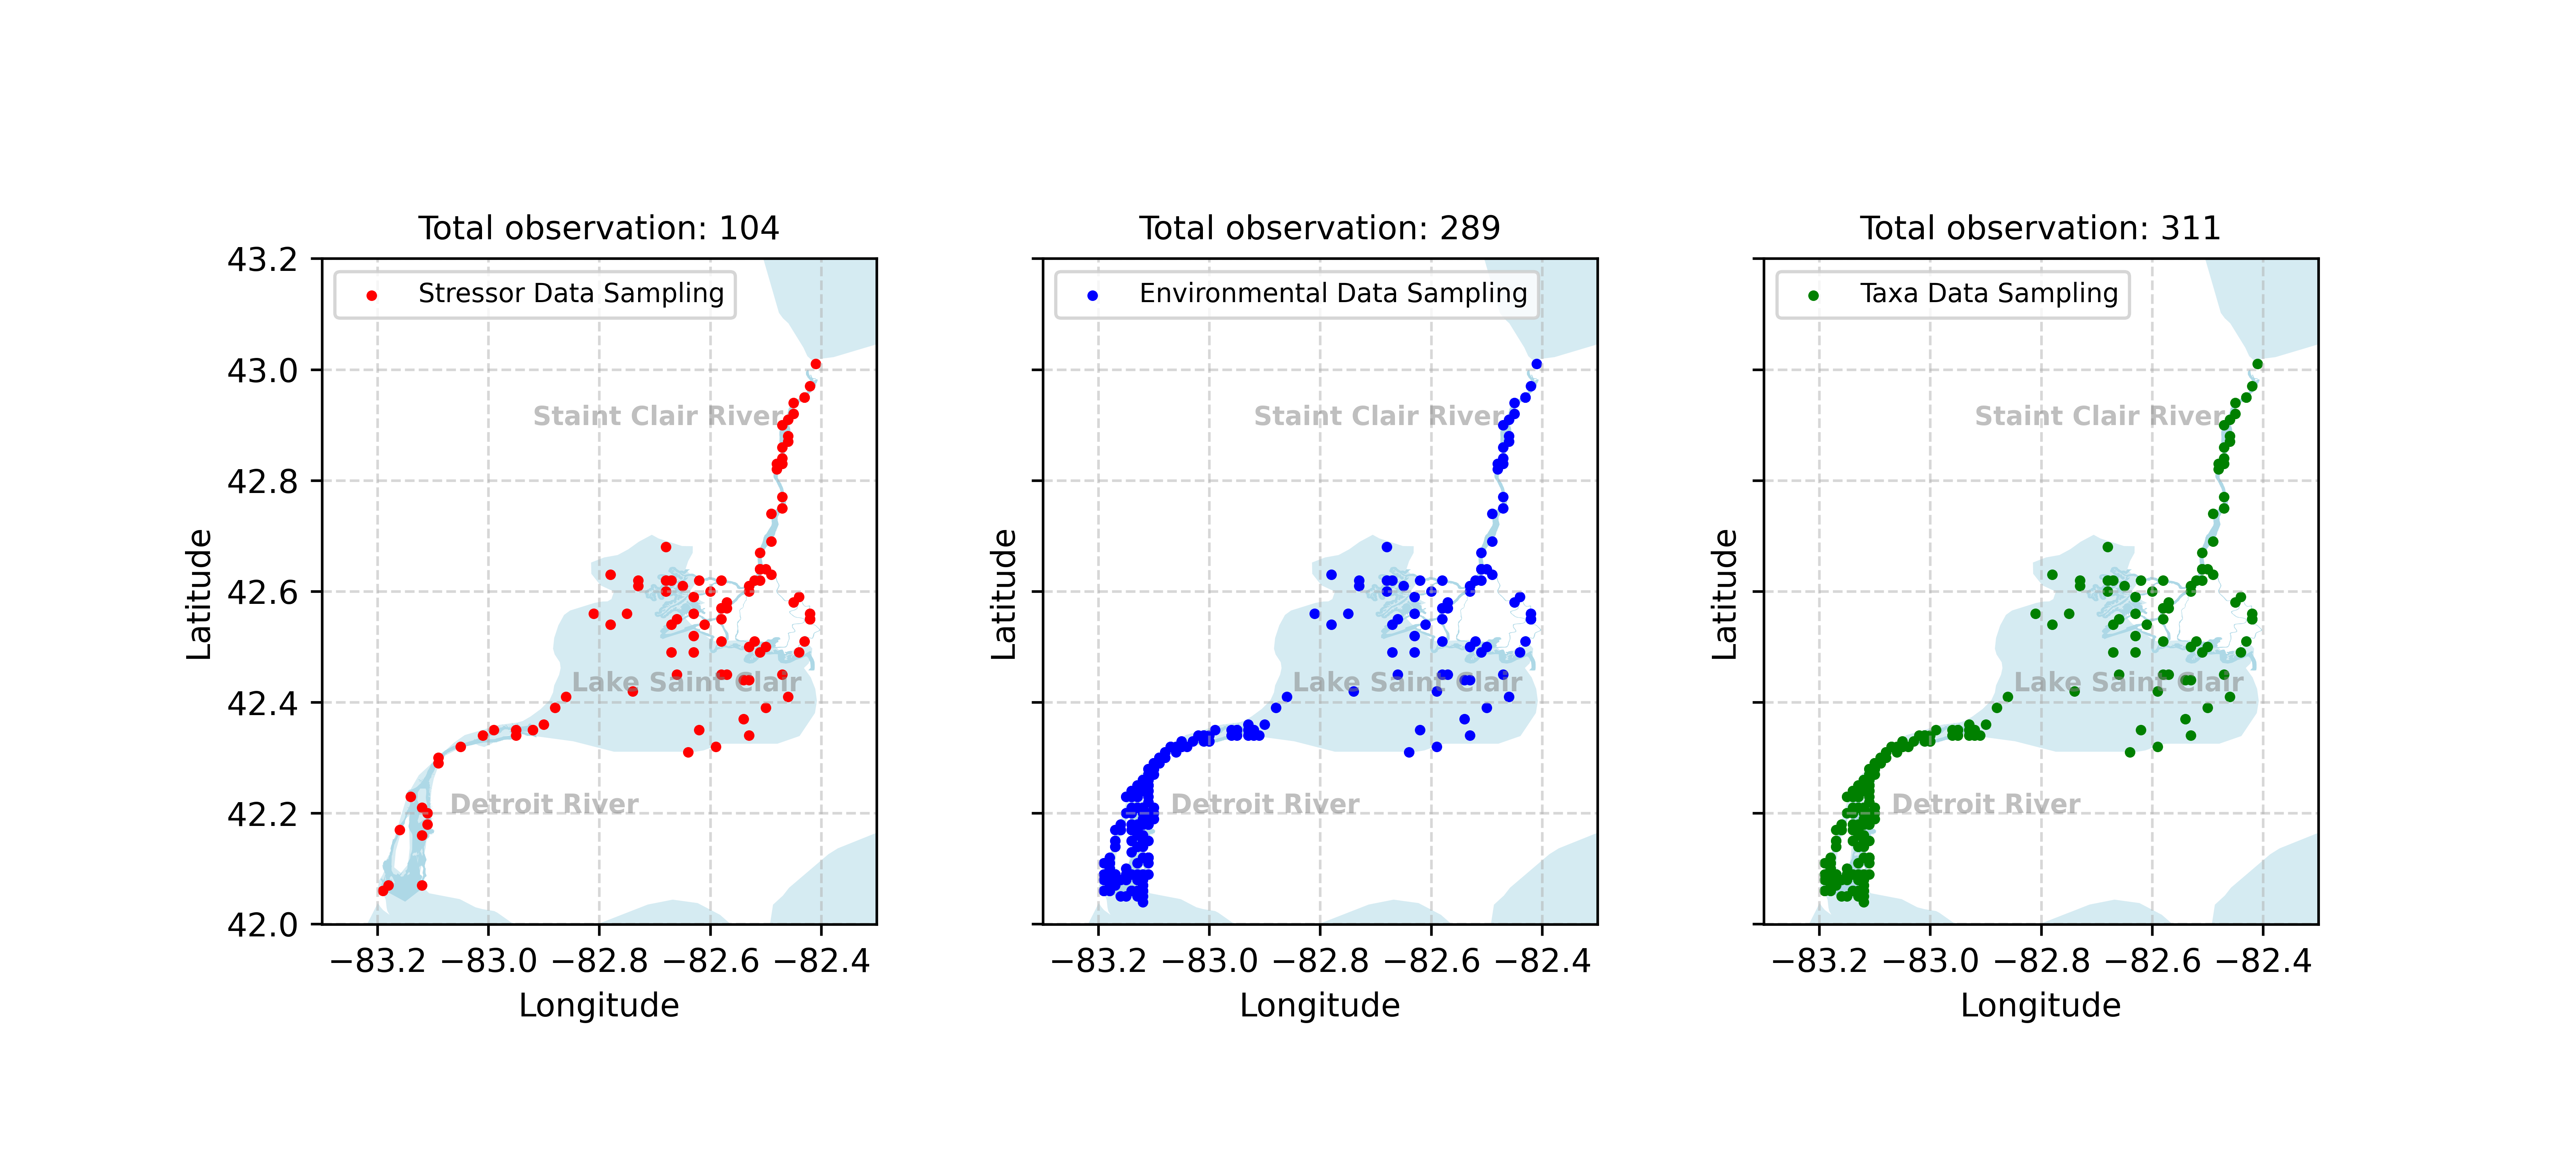
\includegraphics[width=1\textwidth]{../results/different_data_sampling_locations.png}
    \caption{\textit{Map of the SCDRS showing the distribution of locations for which contaminants(left - red points),
environmental covariates (centre - blue points) and zoobenthic data (right - green points) were collected.
Different samples were collected in both temporal and spatial dimensions}}
    \label{fig:different_data_sampling_locations}
\end{figure}

Figure \textcolor{blue}{\ref{fig:different_data_sampling_locations}} shows the numbers
and locations of observations in each dataset.
Note that some locations may be sampled in different
years and only a StationID
\footnote{StationID uniquely identifies a sampling site in both temporal and spatial dimensions.}
(rather than a geographical location) can be
used to confirm the identity of a sampling site.
The three datasets with different types of information (environmental, taxonomic, and stressor) differed in
sample sizes of their observations (row counts).
The stressor dataset contains the fewest observations (104), while the taxonomic and environmental datasets
contain more observations (289 or more).
To prepare a complete dataset for preliminary analysis,
the three datasets were merged by StationID using inner-join operations,
resulting in a comprehensive dataset with 104 observations containing taxonomic, 
environmental, and stressor data across the Lake Huron-Erie Corridor.

This sample size misalignment will be resolved when complete data becomes available in the near future.
Since sample size is the primary difference between current and forthcoming datasets,
the preliminary analysis framework is designed for easy scalability
when additional data becomes available.

\subsection{Large River Case Study: extra water velocity data in Detroit River}
Previous work \cite{Zhang2008} identified limitations in model performance due to insufficient environmental variable coverage.
In a Detroit River-focused analysis \cite{Zhang2008},
a new environmental variable—bottom \textbf{water velocity}—was added,
which was derived by Dr. S. Reitsma using a three-dimensional water flow model.
The focused analysis demonstrated that water velocity is a critical environmental variable for
controlling environmental variation.
Therefore, the Detroit River will serve as a focused study area with water velocity data included,
and it will be conducted once complete stressor data becomes available.

\subsection{Environmental attributes and samples}

Across the three SCDRS surveys, 
location information (longitude and latitude recorded via GPS readings) and 5 environmental attributes
were measured at each sampling site.

\textbf{Temperature ($^\circ$C)} and \textbf{dissolved oxygen concentration ($mg/L$)} were measured using a Hydrolab multimeter. 
\textbf{Water depth ($m$)} was recorded from the Ponar rope.
\textbf{Loss on ignition (\%)} and \textbf{median particle size (phi-units)} were determined during sediment 
processing but are treated as environmental attributes due to their fundamental roles in habitat
characterization (details on their analysis are provided in a later subsection).
% \footnote{Although loss on ignition and median particle size are derived from sediment samples, 
% they are considered environmental variables because they reflect essential physical and chemical habitat features.}
\textbf{Water velocity ($m/s$)} was estimated for the Detroit River area across the three surveys,
displayed in the Table \textcolor{blue}{\ref{tab:environmental_attributes}} along with other cross-corridor attributes.



\begin{table}[htbp]
\centering
\caption{Environmental Attributes}
\label{tab:environmental_attributes}
\begin{tabular}{|>{\centering\arraybackslash}m{4cm}|>{\centering\arraybackslash}m{11cm}|}
\hline
\textbf{Attribute} & \textbf{Ecological Relevance} \\[0.5em]
\hline
Temperature ($^\circ$C) & Controls metabolic rates and organism distribution patterns. \\[0.5em]
\hline
Dissolved Oxygen Concentration ($mg/L$) & Determines survival and excludes oxygen-sensitive taxa when low. \\[0.5em]
\hline
Water Depth ($m$) & Affects light penetration and benthic habitat availability. \\[0.5em]
\hline
Loss on Ignition (\%) & Indicates organic matter content and food availability for benthos. \\[0.5em]
\hline
Median Particle Size (phi-units) & Determines substrate stability and habitat suitability for taxa. \\[0.5em]
\hline
Water Velocity \(^*\) ($m/s$) & Controls flow regime and determines which taxa can colonize sites. \\[0.5em]
\hline
\end{tabular}
\begin{flushleft}
\footnotesize
\textit{(i)} \(^*\) Water velocity was estimated from the model by Dr. S. Reitsma (Detroit River area only, 225 observations) \cite{Zhang2008}.
\\ \textit{(ii)} Other environmental attributes were measured at all sampling sites across the entire survey area (311 observations).
\\ \textit{(iii)} All three surveys (1991, 1999, 2004) followed identical collection protocols and were merged for comprehensive temporal analysis.
\end{flushleft}
\end{table}

These attributes are commonly used to describe baseline environmental conditions in aquatic habitats,
as they are primarily governed by natural physical processes that 
influence taxonomic composition \cite{Davies2006, Turner1989PatternProcess}.

By including these variables as covariates to partially partition the zoobenthic community composition,
we can partially control for natural variation contributed by habitat characteristics, thereby 
isolating the effects of anthropogenic stressors in subsequent analyses 
of community composition patterns.

% However, it is important to note 
% that certain attributes (e.g., organic matter content or temperature) may also be
% indirectly influenced by anthropogenic activities in some settings. 
% Care was taken to interpret their roles in the context of site history and
% land use, but in general, these variables serve as key descriptors of the 
% underlying habitat conditions independent of direct contamination or disturbance.


\subsection{Taxonomic attributes and samples}
The zoobenthos were collected with a Ponar grab sampler. 
After considering the fullness of each grab and the removing of fine materials,
the team applied multiple grabs at each site until a total volume of 2\(L\) sediment was collected.
The sediment samples for organic and metals analysis were preserved in corresponding professional containers, 
all these samples were stored frozen.

One zoobenthic sample replicate from each site was randomly selected and processed, 
while the other two were archived. Samples were sieved into size fractions (4 mm, 1 mm, 0.5 mm, 0.25 mm), 
then elutriated to separate lighter detritus and animals from inorganic sediments. 
Each fraction was sorted under a microscope and organisms were identified to the lowest 
possible taxonomic rank using standard keys. Zoobenthos were preserved in 70\% ethanol in 
labeled vials and archived at the University of Windsor\cite{Zhang2008}.
Immediately after the initial sorting of samples, ten samples were randomly selected to assess the sorting efficiency. 
One sample had a sorting efficiency of 91\%,
while the remaining samples had efficiencies of 96\% or higher.

Specifically, there were 16 taxa recorded from the sediment samples, as shown in the table \textcolor{blue}{\ref{tab:taxonomic_variables}}.
According to their creature characteristics and preferred habitat, 
these taxa can be gently divided into three groups according to their preferred habitat.

\begin{table}[htbp]
\centering
\caption{Benthic Taxa and Preferred Habitat Features}
\label{tab:taxonomic_variables}
\begin{tabular}{|>{\centering\arraybackslash}m{3cm}|>{\centering\arraybackslash}m{5cm}|>{\centering\arraybackslash}m{4cm}|}
\hline
\textbf{Taxa} & \textbf{Explanation} & \textbf{Preferred Habitat} \\
\hline
Nematoda         & Roundworms                   & \multirow{6}{*}{Broad} \\
Chironomidae     & Non-biting midges (larvae)   &  \\
Ceratopogonidae  & Biting midges                &  \\
Amphipoda        & Small crustaceans (scuds)    &  \\
Acari            & Aquatic mites                &  \\
Hydrozoa         & Small predatory animals      &  \\
Gastropoda       & Snails and slugs             &  \\
\hline
Oligochaeta      & Aquatic segmented worms      & \multirow{6}{*}{Depositional zone} \\
Hexagenia        & Mayfly genus (larvae)        &  \\
Dreissena        & Zebra/quagga mussels         &  \\
Hirudinea        & Leeches                      &  \\
Turbellaria      & Flatworms                    &  \\
Sphaeriidae      & Fingernail clams             &  \\
\hline
Caenis           & Mayfly genus (larvae)        & \multirow{3}{*}{Erosional zone} \\
Hydropsychidae   & Net-spinning caddisflies     &  \\
Other Trichoptera& Other caddisfly families     &  \\
\hline
\end{tabular}
\end{table}

\begin{itemize}
    \item \textbf{Broad habitat:} Characterized by a wide range of environmental tolerance. Species in this group can inhabit both depositional and erosional areas, adapting to variable flow velocities, sediment types, and oxygen levels.
    
    \item \textbf{Depositional zone:} Areas with low to moderate water velocity where fine sediments (silt, clay, and organic matter) settle. These habitats often exhibit higher organic content and reduced oxygen penetration, favoring taxa adapted to softer substrates and potentially more enriched nutrient conditions.
    
    \item \textbf{Erosional zone:} Areas with higher flow velocity, coarser substrates (gravel, cobble, or sand), and well-oxygenated water. These habitats support taxa adapted to cling or attach to stable surfaces and withstand stronger currents.
\end{itemize}





\subsection{Stressors attributes and samples}

Sediment samples from each site were thoroughly mixed to ensure homogeneity. The homogenized samples were then split into separate portions for different analyses, including median particle size, total organic carbon (TOC), organic contaminants, and metals.

\begin{itemize}
    \item \textbf{Particle Size:} Median particle size analysis was performed by sieving dried sediment through a series of sieves of decreasing mesh size. Each size fraction was weighed and described using phi units ($\phi = -\log_2 d$), where $d$ is particle size in mm.
    \item \textbf{Total Organic Carbon (TOC):} Sediment TOC(\%OC) was determined using loss on ignition (LOI). Pre-weighed, dried sediment samples were combusted at 450$^\circ$C for 24 hours, and organic carbon was determined gravimetrically by subtracting the remaining mass.
    \item \textbf{Organic Contaminants:} The concentrations of organic contaminants (including 1245-TCB, 1234-TCB, QCB, HCB, OCS, p,p'-DDE, p,p'-DDD, mirex, Heptachlor Epoxide, total PCB)
     were measured using a gas chromatograph equipped with a 63Ni electron capture detector, following standard operating procedures.
    \item \textbf{Metals:} Metal concentrations (including Al, As, Ca, Cd, Co, Cr, Cu, Fe, Mn, Ni, Pb, and Zn) were analyzed using an Inductively Coupled Plasma Optical Emission Spectrophotometer (ICP-OES). For total mercury (Hg), an atomic absorption spectrophotometer (AAS) was used with a vapor generation accessory for increased sensitivity. Liquid samples were introduced into the instrument for metal analysis.
\end{itemize}

\begin{table}[htbp]
\centering
\caption{Sediment Stressors and Classifications}
\label{tab:stressors}

\renewcommand{\arraystretch}{1.2}
\begin{tabular}{|>{\centering\arraybackslash}m{2.5cm}|>{\centering\arraybackslash}m{7cm}|>{\centering\arraybackslash}m{3cm}|}
\hline
\textbf{Variable} & \textbf{Description} & 	\textbf{Type} \\
\hline
\multicolumn{3}{|c|}{\textbf{Metals (mg/kg sediment)}} \\
\hline
Al & Aluminum concentration (nontoxic) & Earth Element \\
Ca & Calcium concentration (nontoxic) & Earth Element \\
Fe & Iron concentration (nontoxic) & Earth Element \\
K & Potassium concentration (nontoxic) & Earth Element \\
Mg & Magnesium concentration (nontoxic) & Earth Element \\
Na & Sodium concentration (nontoxic) & Earth Element \\
As & Arsenic concentration (pollutant) & Trace Metal \\
Bi & Bismuth concentration (pollutant) & Trace Metal \\
Cd & Cadmium concentration (pollutant) & Trace Metal \\
Co & Cobalt concentration (pollutant) & Trace Metal \\
Cr & Chromium concentration (pollutant) & Trace Metal \\
Cu & Copper concentration (pollutant) & Trace Metal \\
Hg & Mercury concentration (highly pollutant) & Trace Metal \\
Mn & Manganese concentration (pollutant) & Trace Metal \\
Ni & Nickel concentration (pollutant) & Trace Metal \\
Pb & Lead concentration (pollutant) & Trace Metal \\
Sb & Antimony concentration (pollutant) & Trace Metal \\
V & Vanadium concentration (pollutant) & Trace Metal \\
Zn & Zinc concentration (pollutant) & Trace Metal \\
\hline
\multicolumn{3}{|c|}{\textbf{Organic Carbon (mg/kg sediment)}} \\
\hline
\%OC & Organic carbon content & Binding agent \\
\hline
\multicolumn{3}{|c|}{\textbf{Organic Contaminants (mg/kg sediment)}} \\
\hline
1245-TCB & 1,2,4,5-Tetrachlorobenzene (hydrocarbon pollutant) & Industrial compound \\
1234-TCB & 1,2,3,4-Tetrachlorobenzene (hydrocarbon pollutant) & Industrial compound \\
QCB & Pentachlorobenzene (hydrocarbon pollutant) & Industrial compound \\
HCB & Hexachlorobenzene (hydrocarbon pollutant) & Industrial compound \\
OCS & Octachlorostyrene (hydrocarbon pollutant) & Industrial compound \\
p,p'-DDE & Dichlorodiphenyldichloroethylene (pesticide) & Organochlorine \\
p,p'-DDD & Dichlorodiphenyldichloroethane (pesticide) & Organochlorine \\
mirex & Mirex (pesticide) & Organochlorine \\
Heptachlor Epoxide & Heptachlor Epoxide (pesticide) & Organochlorine \\
total PCB & Total polychlorinated biphenyls & Sum of all PCBs \\
\hline
\end{tabular}
\end{table}

Quality assurance and chemical analyses were performed in collaboration with the Great Lakes
Institute for Environmental Research (GLIER) at the University of Windsor\cite{Zhang2008}.
Among the chemical variables analyzed, major earth elements (Al, Ca, Fe) are generally non-toxic at typical environmental concentrations, reflecting natural sediment composition. 
However, elevated levels from industrial activities can make them potential stressors, 
leading to difficulties in assessing their impacts due to naturally high background concentrations.

In contrast, trace metals (As, Bi, Cd, Co, Cr, Cu, Hg, Mn, Ni, Pb, Sb, V, Zn) are 
anthropogenic pollutants that bioaccumulate in sediments and cause toxicity in benthic organisms.

Persistent organic pollutants (PCBs, QCB, HCB, OCS, p,p'-DDE, p,p'-DDD, mirex, 
Heptachlor Epoxide) from industrial activities and pesticide use persist in sediments 
and accumulate in food webs, causing chronic effects on aquatic organisms.

Percent organic carbon (\%OC) from decomposed organic matter influences contaminant 
binding and bioavailability, modulating the ecological impact of other pollutants.

By distinguishing between natural major elements (Al, Ca, Fe), trace elements (Co, Mn, Sb, V), 
toxic metals (As, Cd, Cr, Cu, Ni, Pb, Zn), the highly toxic mercury (Hg), organic matter content (\%OC), 
and persistent organic pollutants (including pesticides and industrial compounds), 
these measurements enable a more comprehensive assessment of the sediment stress level and 
its ecological implications for the benthic community.



\section{Literature Review}

\subsection{Sediment Contamination Assessment}

Sediment contamination assessment serves as a fundamental tool for understanding
and protecting aquatic ecosystem health, as contaminated sediments pose significant
risks to benthic communities and serve as long-term sources of pollutants 
that can affect entire food webs
\cite{MacDonald2000SedimentGuidelines, Burton2010MultipleStressors}.
Sediments act as major repositories for a wide range of contaminants 
including heavy metals, persistent organic pollutants, and industrial
chemicals, making their assessment critical for evaluating ecological 
risks and informing environmental management decisions
\cite{Chapman1990SedimentTriad, USGS_SedimentAssociatedContaminants_2019}.

Some popular evaluation methods include contaminant index-based approaches such as the Enrichment Factor (EF) and the
Geoaccumulation Index (Igeo).
These index-based approaches provide pollution scores relative to known background or reference values, 
often focusing on individual or selected chemical elements \cite{Birch2022Review} (Birch, 2022). 
For example, the Igeo index \cite{BIRCH2013282} (Birch, 2013) compares current concentrations to pre-industrial levels,
while the EF index compares current concentrations to regional background levels.
However, these approaches are limited by their reliance on accurate background 
concentration estimates and consideration of only a few chemical elements. 
When applied to datasets with many variables, they become less effective 
as they treat elements independently and fail to capture multivariate 
contamination patterns \cite{Grunfeld2005Outliers}.

A more general class of evaluation methods relies on multivariate ordination and data reduction techniques. 
These data-driven approaches consider all chemical variables simultaneously, revealing interaction patterns 
through dimensionality reduction without requiring background or reference values, thus avoiding the 
challenge of defining appropriate benchmarks \cite{Ciborowski2005ZoobenthicIndicators, Reynoldson1997ReferenceCondition}. 
However, such methods often yield composite axes or scores that lack intuitive interpretation and clear 
pollution thresholds, limiting their ability to provide comparable pollution categories like index-based 
methods \cite{Reimann2008Chemometrics}. This interpretability challenge has been recognized in ecological 
assessment contexts, where practitioners need actionable thresholds for management decisions 
\cite{Reynoldson1999RCA}.

Turn to large river and lake ecosystems, various pollution sources contribute to a complex array of contaminants,
escalating the need for approaches that can handle complex, multivariate contamination patterns.
Considering there are 30 stressor variables in my project and many of them share 
common pollution sources and interact via similar transport mechanisms,
a data-driven and multivariate approach is more suitable to capture the contamination levels and patterns.
Some ordination methods, such as Principal Component Analysis (PCA), can effectively reduce dimensionality and 
eliminate redundancy among correlated variables \cite{Zitko1994PCA}.
In addition to reducing dimensionality and eliminating redundancy,
advanced PCA methods can also enhance interpretability by incorporating variable weights \cite{Delchambre2015} (Delchambre, 2015) or spatial information \cite{Harris2011GWPCA} (Harris et al., 2011).,
making it possible to derive more meaningful contamination scores.



\subsection{Control of confounding environmental gradients}
In researching relationships between zoobenthic community composition and 
sediment contamination levels, naive associations can be confounded by environmental conditions
that are correlated with community composition or even contamination.
This induces omitted-variable bias and can either inflate or mask the true signal we seek 
for the zoobenthic condition index (ZCI). Accordingly, quantify the unique contribution of 
sediment contamination to community composition, after conditioning on measured environment,
is essential for deriving a reliable and interpretable ZCI.

To overcome this confounding issue, some common fixes include: \textit{(1) regression adjustment / partial regression; (2) variance partitioning; (3) blocking / stratification} \cite{Eberhardt1991FieldStudies, Wiens1995AccidentalImpacts}.
Approaches (1) and (2) are most often used in ecological regression as adjustments to the naïve model, whereas (3) is more common in experimental designs.
The third approach represents a design/estimator-based solution that mitigates latent confounding when environmental information is limited or unaddressed \cite{Byrnes2025CausalInference}.

Within the regression framework, adjustments are useful for statistically disentangling environmental influences \cite{Legendre2008VariationPartitioning}.
However, model performance can be sensitive to the sampling configuration and to the explanatory power of predictors \cite{Legendre2010Limitations,Fischer2018Uncertainty}.

Simulation studies show that model-revealed relationships depend not only on the true ecological relationships but also on the sampling--environmental distribution (SED), underscoring the importance of evenness and representativeness in sampling design \cite{Fischer2018Uncertainty}.
These limitations produce high uncertainty in estimates when any of the following occur: missing environmental predictors, poor coverage across environmental gradients, or insufficient sample size \cite{Eberhardt1991FieldStudies}.

Experimental designs can mitigate these issues when regression adjustment is not feasible, and analytical tools such as clustering or stratification can make the design more objective and data-driven \cite{Wiens1995AccidentalImpacts}.
However, these designs are also subject to SED and sample-size constraints.

A notable avenue is to infer \textit{counterfactual outcomes} for the response variable conditional on specified environmental gradients; these outcomes represent the environmentally deterministic component of the response \cite{Larsen2019CausalAnalysis, Byrnes2025CausalInference}.
This approach combines regression adjustment with experimental design: initial data for learning the counterfactual surface are selected via design (e.g., blocking/stratification), and the subsequent inference step uses trained regression models to estimate these deterministic counterfactual outcomes.


\subsection{Zoobenthic Community Composition Measurement}

Zoobenthic community composition measurement depends fundamentally on 
how we define and quantify the community, making it nearly impossible to establish a 
perfect measurement framework in real ecological systems \cite{Tampo2021Bioindicators}. 
Common descriptors of zoobenthic community composition include species richness, abundance, and biomass, 
which can be used individually or in combination to characterize the community \cite{Sitati2021AbundanceBiomass}. 
Each metric presents trade-offs between the amount of ecological information captured 
and the cost of data acquisition \cite{Menezes2010Trait}. 

The individual organism represents the minimal unit in a zoobenthic community and serves as 
the foundational unit for measuring abundance and biomass. 
While individual responses to external conditions ultimately comprise the community response,
their high variability and inherent stochasticity present significant challenges 
for using single or few individuals to adequately describe community-level responses.
In contrast, taxonomically rich assemblages can better represent community responses by 
averaging out individual-level variability and capturing broader ecological patterns \cite{Menezes2010Trait}.

Beyond the fundamental function of representing community structure, the choice of measurement approach 
depends critically on the study's primary objectives. In this project, the main purpose is to 
assess sediment contamination levels using zoobenthic community indicators \cite{Ciborowski2005ZoobenthicIndicators}.
Rooted in this purpose, we seek measurements that demonstrate sensitivity to contamination gradients—
whether reflecting raw stressor concentrations or evaluated contamination levels—such that 
pollution-sensitive metrics can outperform alternatives in mathematically predicting contamination levels.
However, such forecast-oriented measurements may exhibit limited mechanistic interpretability 
regarding the zoobenthic community composition itself, necessitating caution when 
interpreting results from a biological perspective.
To address this limitation, comprehensive mechanistic investigation of the taxa-based measurements 
and cross-validation with existing ecological knowledge becomes essential \cite{Reynoldson1999RCA}.


\subsection{Quantitative Regression Beyond the Mean and Threshold Detection}
Benefiting from the Central Limit Theorem and classical statistical theory,
mean-based regression has dominated ecological analysis \cite{Cade2003}.
Traditional linear regression performs adequately under weak correlations 
and homogeneous variance, but degrades substantially when these assumptions 
are violated—a common occurrence in ecology due to natural system complexity 
and unmeasurable latent factors. 
% While weighted least squares (WLS) addresses 
% heteroscedasticity through variance weighting, its linearity assumptions 
% still limit ecological applications.

Beyond statistical limitations, mean-based approaches can miss important ecological
patterns, elevating the meaningful investigation of relationships beyond the mean.
Ecological drivers often act in a heterogeneous way across the distribution of
responses, such that effects emerge only under extreme conditions and not in the 
center of the distribution. 
For instance, \cite{Schmidt2012Quantile}(Schmidt et al. 2012)
found that the influence of metal concentration was much stronger 
at higher quantiles of the biological response than on the mean.
Such upper‐tail–specific associations underscore the limitation of 
mean regression approaches when the primary ecological signal lies in extremes.
They thus motivate the use of “mean‐beyond” methods
- such as quantile regression - that can capture 
effects under high-stress or extreme conditions.

Nonlinear and threshold effects are another phenomenon observed in many ecological 
systems \cite{Cade2003} (Cade \& Noon, 2003). 
The concept of ecological thresholds emerged in the 1970s with the recognition 
that ecosystems often exhibit multiple 'stable' states under different conditions 
\cite{Holling1973} (Holling, 1973, as cited in Groffman et al., 2006).  
Peterson et al. \cite{peterson2006ecological} (Peterson et al., 2006) summarized 
three main applications of ecological thresholds: (1) \textbf{ecosystem state shifts} from small driver changes, 
(2) \textbf{critical loads} that ecosystems can absorb without functional changes, and 
(3) \textbf{extrinsic factor thresholds} where large-scale changes modify driver–response relationships.
These ecological recognitions motivate and justify the use of threshold-detecting 
methods in ecological regression modeling.

The threshold usually functions as a crucial decision point for management,
policy, or conservation actions.
Therefore, identifying and validating ecological thresholds is vital in both 
statistical and practical senses. 
Spake et al. \cite{Spake2022} emphasized the importance of \textit{scale}, 
highlighting four dimensions affecting threshold detection: (1) \textbf{grain} (measurement resolution), 
(2) \textbf{extent} (total area or duration covered), (3) \textbf{organizational level} (biological hierarchy), 
and (4) \textbf{analytical method} (statistical approach employed).
Turning to threshold detection, testing their existence and reliability is crucial.  
Daily et al. \cite{Daily2012} (Daily et al., 2012) showed that small sample sizes increase false detections, 
while larger samples improve reliability.  
The sample–environment distribution (SED) strongly influences detection and threshold location, 
with uneven SEDs producing bias.  
The rate of ecological change, whether linear or nonlinear, interacts with the chosen method, 
and user-defined parameters (e.g., quantile \(\tau\), bandwidth) play a critical role.
\section{Methodology}

This methodology section details the overall analytical framework and specific techniques to be employed in this research.

The proposed methodology consists of the following key steps:

\begin{enumerate}
\item Dimension reduction on stressors that produce pollution scores and arranges samples in a low-dimensional pollutant space to reveal main synthetic stressor gradients.

\item Find and prepare least polluted sites, construct an estimator that estimates the counterfactual surface (minimal pollution level) of taxa community composition in environmental space.

\item Ordinate the taxa variables, construct comprehensive measurement for the taxa community.

\item Spatial heterogeneity test and geo-information incorporated for latent environmental variables.

\item Piecewise quantile regression models on ZCI and pollution scores, revealing relations at different quantile levels and detecting thresholds.

\item Step out of the framework, change global factors, like sample size and partitioning samples by biased environmental distribution. Study how the series of estimates would change accordingly.
\end{enumerate}

Various symbols are used throughout this section, including function names, vectors, and matrices. The following table summarizes these symbols:

\begin{table}[!h]
\centering
\caption{Summary of major mathematical symbols and their meanings, organized by subsection.}
\begin{tabular}{lll}
\toprule
\textbf{Subsection} & \textbf{Symbol} & \textbf{Meaning} \\
\midrule
\multirow{7}{*}{\parbox{3cm}{\centering Data Description and Sediment Contamination Assessment}} 
& $m$ & Number of sampled sites \\
& $X \in \mathbb{R}^{m \times 30}$ & Elemental concentration matrix (30 chemical elements) \\
& $E \in \mathbb{R}^{m \times 5}$ & Environmental variable matrix (5 variables) \\
& $T \in \mathbb{R}^{m \times 16}$ & Taxa abundance matrix (16 taxa) \\
& $s \in \mathbb{R}^m$ & Composite stressor score (from PCA) \\
& $p\%$ & Percentage of least stressed sites chosen as reference \\
& $I_{\mathrm{ref}} \in \mathbb{R}^m$ & Indicator: 1 = reference site, 0 = disturbed site \\
\midrule

\multirow{5}{*}{\parbox{3cm}{\centering Reference site clustering and Discriminant Function}} 
& $\mathcal{C}_K$ & Cluster label (taxa composition group) from reference sites \\
& $\hat{\mathcal{C}}_K$ & Predicted cluster label for disturbed sites \\
& $\mathcal{F}_{\mathrm{dis}}$ & Discriminant function mapping $E_{\mathrm{ref}}$ to $\mathcal{C}_K$ \\
& $\delta T_{i,j}$ & Taxa community structure relative to the scale of reference site \\
& $\delta X_{k,j}$ & Stress level relative to group-$k$ reference median \\
\midrule

\multirow{12}{*}{\parbox{3cm}{\centering
    Multivariate Gaussian modeling for constructing Zoobenthic Community Index (ZCI)
 }} 
& $\phi_{\mathrm{Hel}}$ & Hellinger transformation \\
& $\mathcal{R}_k$, $\mathcal{D}_k$ & Sets of reference and disturbed sites in group $k$ \\
& $\boldsymbol{\mu}_k$ & Mean taxa composition vector for group $k$ reference sites \\
& $\boldsymbol{\Sigma}_k$ & Covariance matrix of taxa composition in group $k$ \\
& $\lambda$ & Ridge regularization term \\
& $I_{16}$ & $16\times16$ identity matrix \\
& $\tilde{T}_{k,j}$ & Whitened deviation vector for site $j$ in group $k$ \\
& $\mathrm{ZCI}_{k,j}$ & Scalar Mahalanobis distance from reference centroid \\
& $\mathrm{ZCI}^{(\mathrm{diag})}_{k,j}$ & Diagonal approximation ignoring correlations \\
& $\mathrm{ZCI}^{(1)}_{k,j}, \mathrm{ZCI}^{(2)}_{k,j}$ & First two components of multi-dimensional ZCI \\
& $\mathrm{ZCI}^\star_{k,j}$ & 0--100 scaled ZCI score \\
& $V_k$ & PCA loading matrix from whitened reference deviations \\
\midrule

\multirow{4}{*}{\parbox{3cm}{\centering
    Spatial basis expansion for spatial predictors
}} 
& $x_i, y_i$ & Spatial coordinates of site $i$ \\
& $D \in \mathbb{R}^{m \times m}$ & Euclidean distance matrix(symmetrical) between sites \\
& $A \in \mathbb{R}^{m \times m}$ & Double-centered distance matrix from truncated distance matrix \\
& $S_{\text{sel}} \in \mathbb{R}^{m \times d}$ & Selected eigenvectors for explaining spatial variation (\(d < m\)) \\
\midrule

\multirow{7}{*}{\parbox{3cm}{\centering Quantile regression modeling}} 
& $\mathcal{F}_{k}$ & Regression function linking ZCI and spatial features to stress level \\
& $\delta X\mid Z, S_{\text{sel}}$ & Relative stress level given ZCI and spatial features \\
& $Q_{\delta X\mid Z, S_{\text{sel}}}^{(k)}(\tau \mid z, s)$ & Conditional $\tau$-quantile of $\delta X$ given ZCI and spatial features \\
& $f_{k, \tau} (z, s)$ & Quantile regression function for group $k$ at quantile $\tau$ \\
& $\kappa_m$ & Fixed breakpoint in piecewise regression \\
& $\gamma_{m,\tau}^{(k)}$ & Slope change after breakpoint $\kappa_m$ \\
& $\hat \theta_{\tau}^{(k)}$ & Estimated parameter for quantile regression \\
\midrule

\multirow{3}{*}{\parbox{3cm}{\centering Hypothesis testing for degradation}} 
& $F_{\delta X\mid Z}^{(k)}(x \mid z)$ & Conditional CDF of stress level given ZCI \\
& $x_k^*$ & Group-$k$ stress threshold for degradation classification \\
& $p$ & One-sided $p$-value for degradation test \\
\bottomrule
\end{tabular}
\end{table}


At the initial stage, the whole information about the sites can be shown in the matrix form:
\[
\left[
\begin{array}{ccc}
X & E & T
\end{array}
\right]
\in
\mathbb{R}^{m \times (30 + 5 + 16)}
\]
where
\(X \in \mathbb{R}^{m \times 30}\) (elemental concentrations),
\(E \in \mathbb{R}^{m \times 5}\) (environmental variables),
and
\(T \in \mathbb{R}^{m \times 16}\) (taxa abundances).

% orginal workflow framework figure
% \begin{figure}[!h]
%     \centering
%     \begin{minipage}{0.8\textwidth}
%         \centering
%         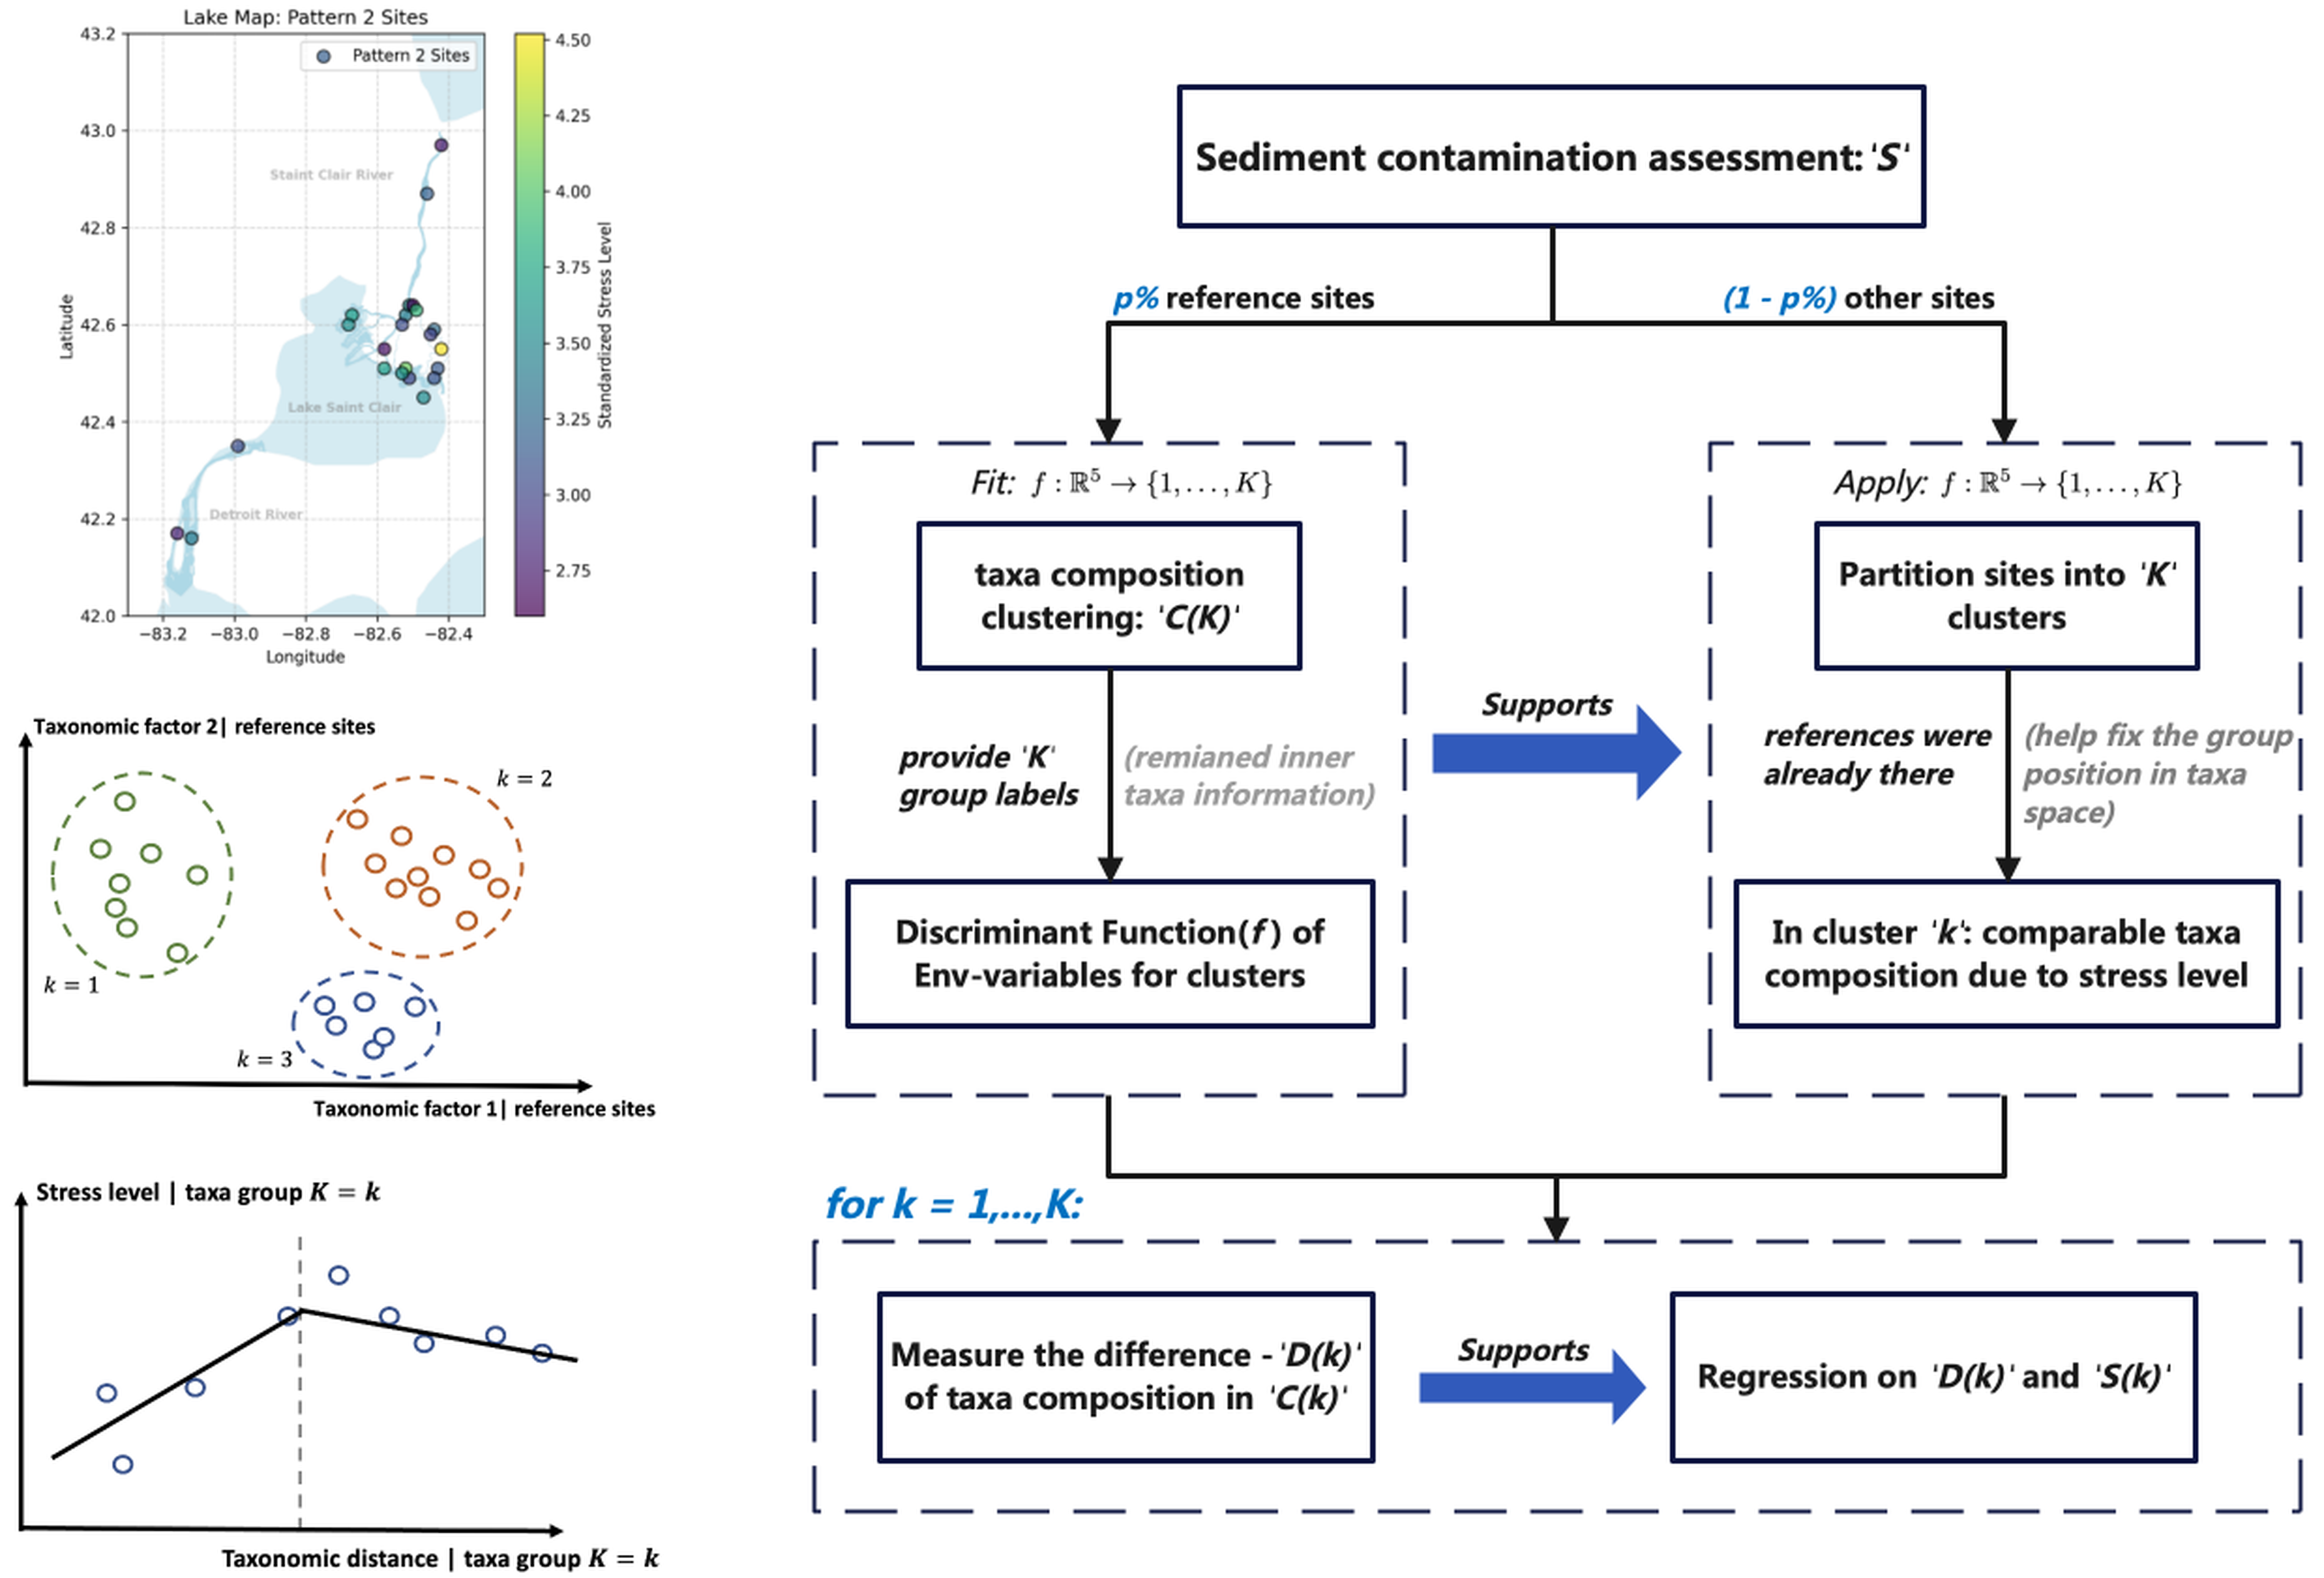
\includegraphics[width=\textwidth]{../results/workflow_of_general_workframe_part1.png}
%         \vspace{0.5em}
%         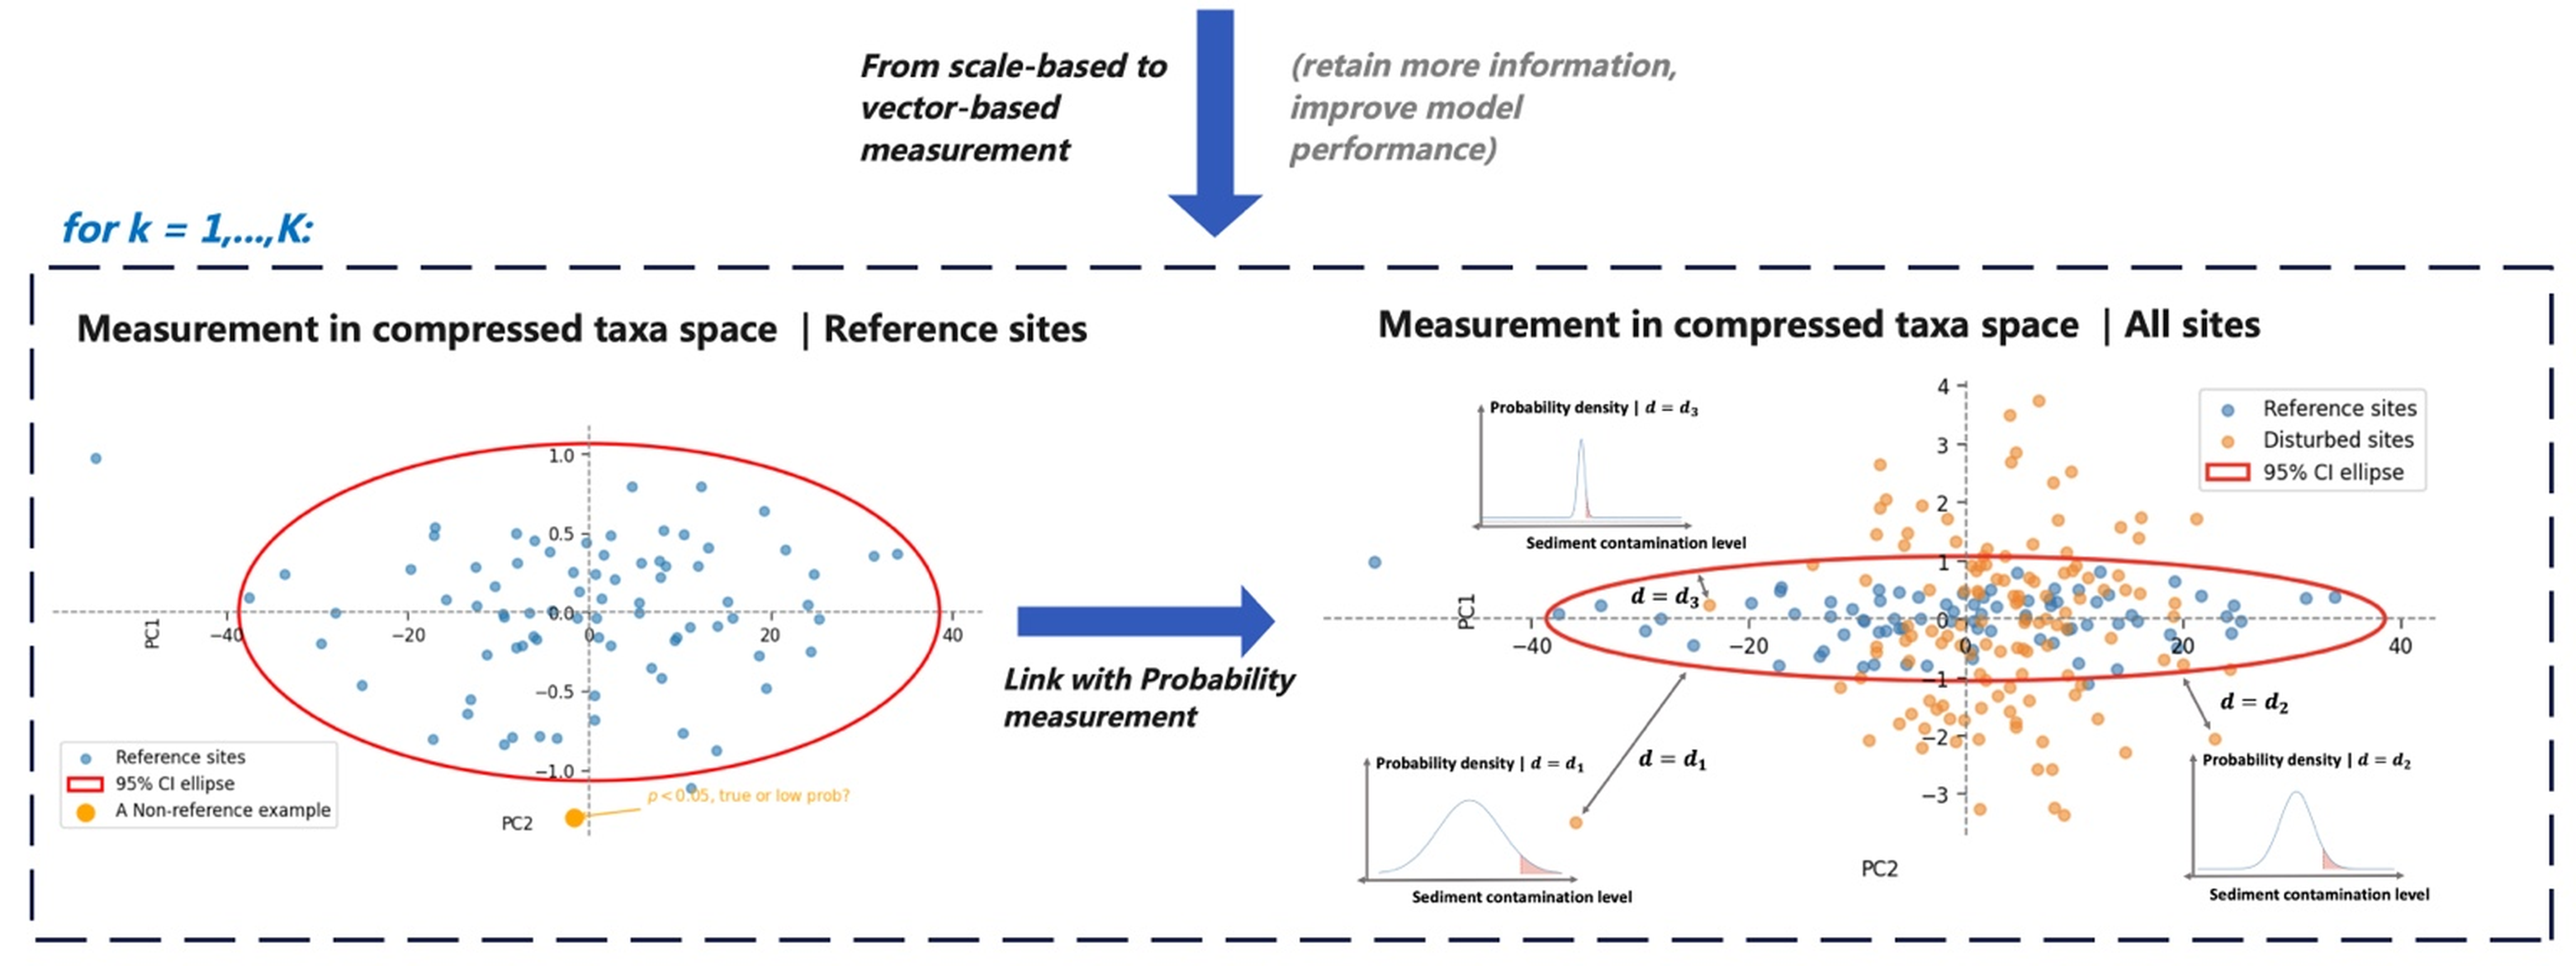
\includegraphics[width=\textwidth]{../results/workflow_of_general_workframe_part2.png}
%     \end{minipage}
%     \caption{Overview of workflow for the proposed methodology.}
%     \label{fig:workflow_of_general_workframe_parts}
% \end{figure}
\begin{figure}
\centering
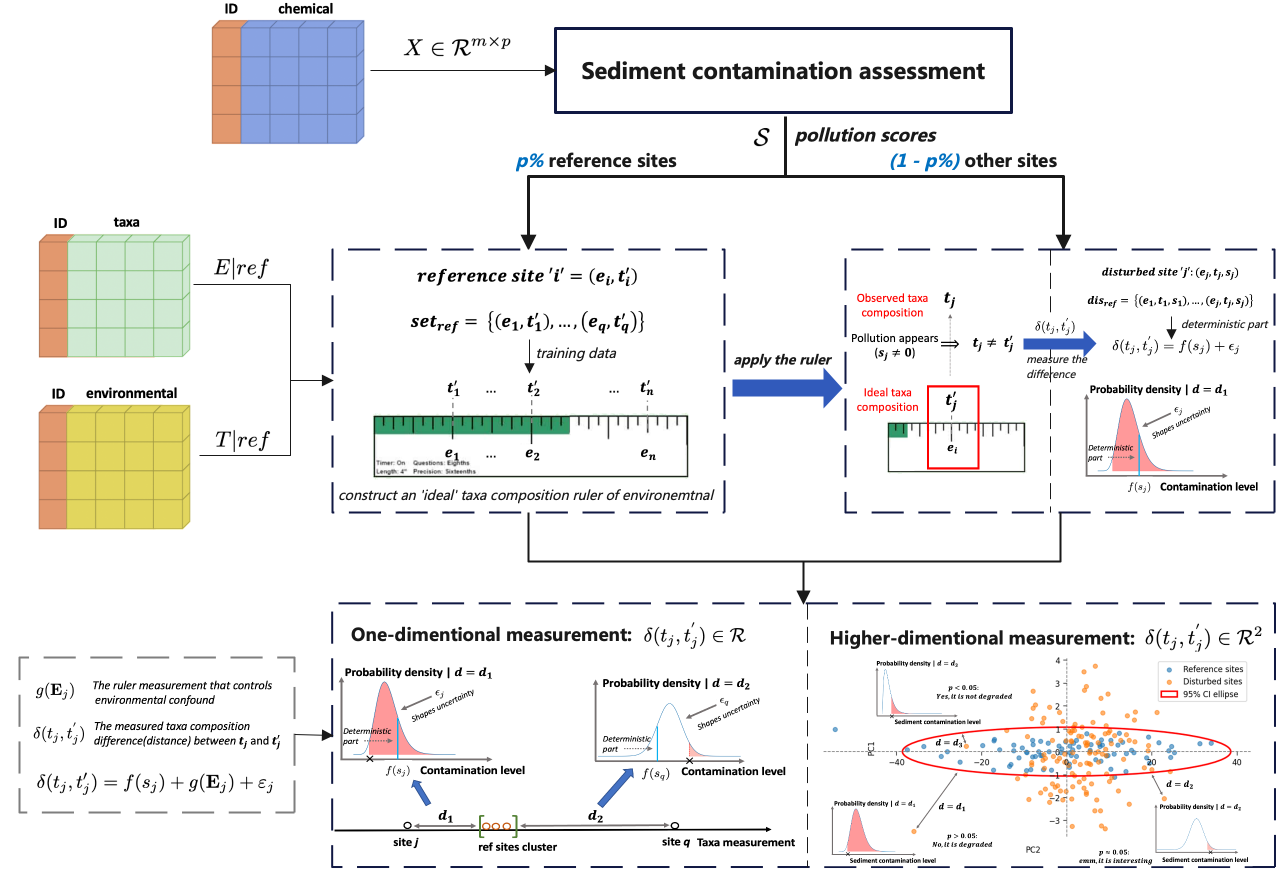
\includegraphics[width=0.8\textwidth]{../results/ideas_visualization/overall_framework.png}  
\caption{\textit{Overview of workflow for the proposed methodology.}}
\end{figure}
\subsection{Find Reference Sites - Sediment Contamination Assessment}

\begin{tcolorbox}[colback=white!95!gray, colframe=white!20!orange, 
    title = \textbf{External Reference: Data-driven PCA-based Pollution Assessment}]
    Detailed methodology for sediment contamination assessment has been developed separately.
    The method report that is under development is available at:
    \begin{itemize}
        \item \href{https://drive.google.com/file/d/1L43eq924ydxNeLgRYH4EsfJd8nvNVOf9/view}
        {Click to access: Method report draft}
    \end{itemize}
\end{tcolorbox}


To assess the sediment contamination and find the reference sites, we need to compute a composite stressor score \(s\) based on the chemical data.

Let \(m\) be the number of sampled sites and \(X \in \mathbb{R}^{m \times 30}\) denote the matrix of chemical element concentrations (each row represents a site and each column represents an element).
Doing a principal component analysis (PCA) on \(X\) transforms it into a set of uncorrelated and high variation-loading components \(Z\).
On top of the \(Z\), we can select \(k\)(\(< 30\)) proper components with defined criteria to cover the most variation in pollutant elements
and define a composite stressor score \(s \in \mathbb{R}^{m}\)
by summing or weighting the selected raw principal components or their normalised variants:


\begin{enumerate}
    \item \textbf{Principal component reduction} – Apply principal component analysis (PCA) to \(X\).  PCA transforms \(X\) into a set of uncorrelated components \(Z = X W\), where \(W \in \mathbb{R}^{30\times k}\) holds loadings of the first \(k\) principal components.

    \item \textbf{Composite stress score} – Let \(Z = [\,z_1,\dots,z_k\,]\) with \(z_i \in \mathbb{R}^{m}\) the vector of scores on the \(i\)-th principal component. 
     Define a composite stressor score \(s \in \mathbb{R}^{m}\) by summing or weighting the selected raw principal components:
    \[
    s_j \;=\;\sum_{i=1}^k \omega_i\,z_{i,j}, \quad j \in \{1,\dots,m\}
    \]
    where \(z_{i,j}\) is the \(i\)-th PC score at site \(j\) and \(\omega_i\) are predetermined weights (often set to 1 when components contribute equally).
\end{enumerate}

After computing the composite stressor score, we can add this new information to the originally compound matrix:
\[
\left[
\begin{array}{cccc}
X & E & T & s
\end{array}
\right] 
\in
\mathbb{R}^{m \times (51 + 1)}
\]

This \(s\) vector is used to rank the sites with respect to 
the stress level and filter the pristine reference sites where
human impact is minimal or absent. 
Specifically, we rank sites by \(s\) and retain the least‑stressed \(p\%\) of the sites,
create an indicator vector \(I_{\text{ref}} \in \mathbb{R}^{m}\) where \(I_{\text{ref},j} = 1\) if site \(j\) is a reference site and \(I_{\text{ref},j} = 0\) otherwise.
\[
\left[
\begin{array}{ccccc}
X & E & T & s & I_{\text{ref}}
\end{array}
\right] 
\in
\mathbb{R}^{m \times (52 + 1)}
\]
To this sites with \(I_{\text{ref},j} = 1\), we assume they represent
the ideal taxa composition that is shaped by the given environmental conditions,
supported by the minimal or absent human disturbance.
\[
\left[
\begin{array}{ccccc}
X & E & T & s & I_{\text{ref}} 
\end{array}
\right]_{I_{\text{ref}} = 1}
\in
\mathbb{R}^{(p\% \times m) \times (53)}
\]
Therefore, in this submatrix, the \(X\) matrix only contains the minimal \(p\%\) stress levels across all sites,
controlling the human disturbance on the taxa composition.

\begin{figure}[!h]
\centering
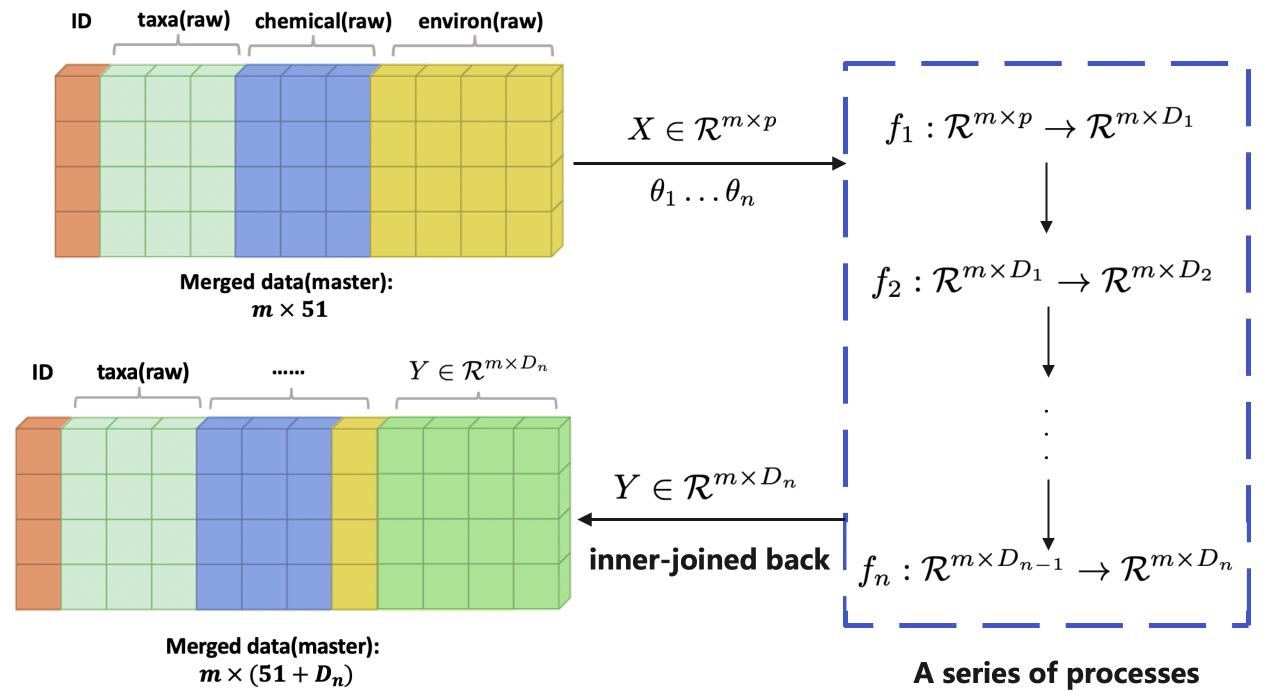
\includegraphics[width=0.8\textwidth]{../results/ideas_visualization/operate_data_throughout2.png}
\caption{\textit{Visualization of how the new information is generated and integrated into the existing matrix.}}
\label{fig:p4_rules_for_data_operation}
\end{figure}

\subsection{Prepare metrics of “ideal” taxa composition - Cluster Analysis on References}
In the matrix
$\left[
\begin{array}{ccccc}
X & E & T & s & I_{\text{ref}} 
\end{array}
\right]_{I_{\text{ref}} = 1}
$, the set of taxa composition \(T_{\text{ref}}\) 
is assumed to be shaped by the environmental variables \(E_{\text{ref}}\),
a well-fitted regression model between the \(E_{\text{ref}}\) and \(T_{\text{ref}}\)
matrices can numerically tell us how the taxa composition is multidimensionally shaped by the environmental variables.

However, considering that the \(E_{\text{ref}} \in \mathbb{R}^{(p\% \times m) \times 5}\) only provides 5 environmental variables,
and there are many other potentially unmeasured and unmeasurable environmental factors, it is nearly impossible to train a fully quantitative
inference model that describes the below relationship well:
\[
\mathcal{F} : E_{\text{ref}}^{(p\% \times m) \times 5} \to T_{\text{ref}}^{(p\% \times m) \times 16}, \quad \text{poorly fitted model}
\]

To solve this issue, we can construct constrained predicted values \(T_{\text{ref}}^{q} (q < 16)\) from the \(T_{\text{ref}}\) matrix, which 
provides limited yet information about the community structure, so that the model $\mathcal{F} : E_{\text{ref}}^{(p\% \times m) \times 5} \to T_{\text{ref}}^{(p\% \times m) \times q}$
can be trained to avoid overfitting and improve its prediction performance.
\[
\mathcal{F} : E_{\text{ref}}^{(p\% \times m) \times 5} \to T_{\text{ref}}^{(p\% \times m) \times q}, \quad \text{improved fitted model}
\]
One ideal way to do this information compression is 
to partition the reference sites into \(K\) different groups via clustering methods.

\[
T_{\text{ref}}^{(p\% \times m) \times q} = \mathcal{C}_K^{(p\% \times m) \times 1}  = clustering(T_{\text{ref}}^{(p\% \times m) \times 16}), \quad \text{where } q = 1
\]

By the clustering analysis and merging the resulting information into the reference-base matrix, the reference-base matrix can be updated as:
\[
\left[
\begin{array}{cccccc}
X & E & T & s & I_{\text{ref}} & \mathcal{C}_K
\end{array}
\right]_{I_{\text{ref}} = 1}
\in
\mathbb{R}^{(p\% \times m) \times (53 + 1)}
\]


Even though the \(C_K\) is computed from the clustering analysis on taxa composition matrix \(T_{\text{ref}}\),
the underlying environmental conditions(\(E_{\text{ref}}\)) are the actual drivers to lead to the clustering results,
based on the fundamental assumption that "the reference taxa-composition is shaped by the environmental conditions".

\begin{figure}[!h]
    \centering
    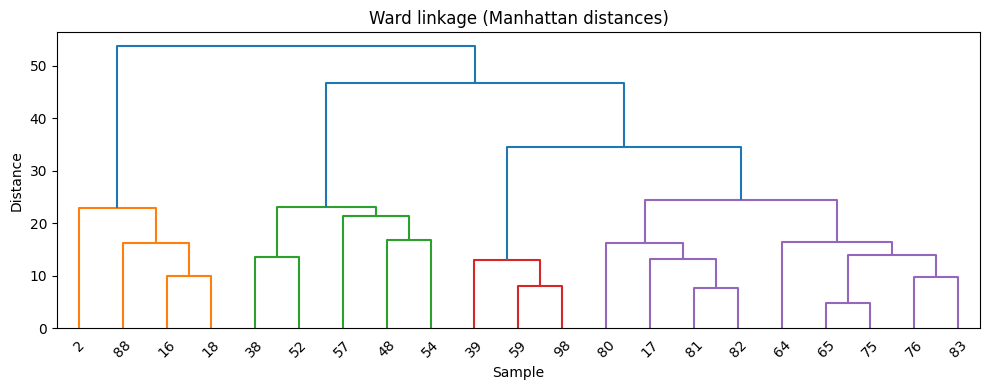
\includegraphics[width=0.8\textwidth]{../presentation/figures/p10_clustering_results.png}
    \caption{\textit{An example of hierarchical clustering results on the taxa composition matrix of the references
    with selected clustering number \(K\).}}
    \label{fig:p10_clustering_results}
\end{figure}


\subsection{Construct “ideal” taxa composition ruler of environmental factors - Fit a Discriminant Function}

\begin{figure}[!h]
\centering
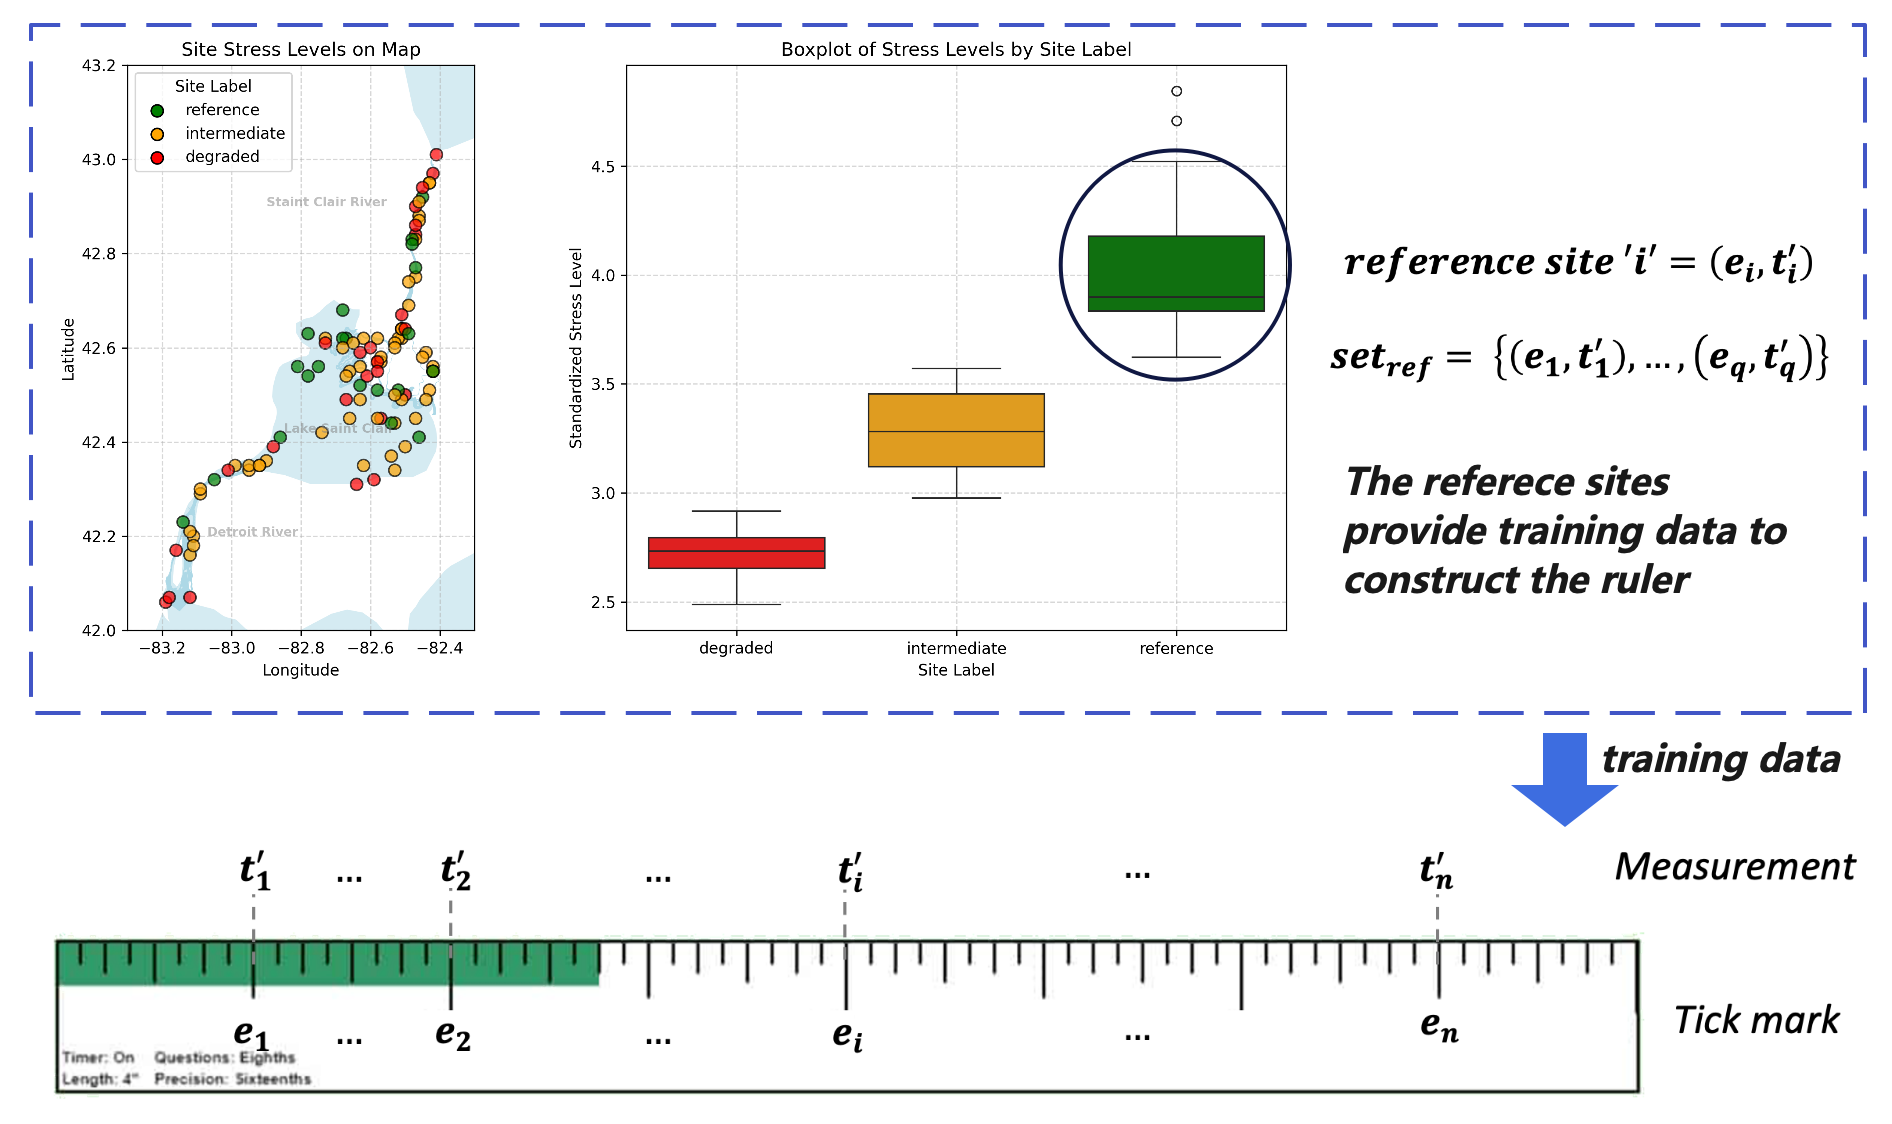
\includegraphics[width=0.8\textwidth]{../results/ideas_visualization/constructing_ruler.png}
\caption{\textit{The reference sites are used as training data to construct this 'ideal' taxa composition ruler.
($t^{'}_{j}$ represents the raw taxa composition of site \(j\), it has not been transformed into the cluster label \(\mathcal{C}_K\) yet.)}}
\label{fig:constructing_ruler}
\end{figure}

At this stage, there are constrained taxa composition information - cluster labels \(\mathcal{C}_K\) that can be used as
response variables in training the environmental-taxa composition regression. 
Specifically, a discriminant function can be fitted here:
\[
\mathcal{F_{\text{dis}}} : E_{\text{ref}}^{(p\% \times m) \times 5} \to \mathcal{C}_K^{(p\% \times m) \times 1}
\]

This discriminant function \(\mathcal{F_{\text{dis}}}\) fitted on the reference sites tells us how the environmental variables - \(E\) roughly shape the 
taxa composition by assigning each site to one of the taxa composition groups \(\mathcal{C}_K\).

During the training stage, the reference sites are partitioned into the \(K\) taxa composition groups, 
helping to fix the group positions in taxa composition space with the pristine taxa composition part in 
each group. \textbf{However, it does not mean there is only pristine taxa composition in each cluster.
When human disturbance appears, the pristine taxa composition should be shifted to a new position in the taxa composition space,
which is how the disturbed sites look like in the same taxa composition space.}

Therefore, these reference sites are partitioned (by clustering) into different clusters to play the role of 'ideal' metrics
on a ruler of taxa composition (by discriminant function), this ruler measures the 'ideal' taxa composition structure that a site should have given its environmental conditions.

An imaginable scenario is that, when we use the fitted \(\mathcal{F_{\text{dis}}}\) as a ruler to measure the taxa composition of sites that are affected by human disturbance,
the measured 'ideal' taxa composition is not equal to the truly observed taxa composition. 
And this difference in taxa composition is caused by the human disturbance, which was measured by the sediment contamination assessment in the previous step.

\subsection{Mark the “ideal taxa composition” for disturbed sites - Apply the Discriminant Function}

Given the fitted discriminant function \(\mathcal{F_{\text{dis}}}\), we can classify the rest \(1 - p\%\) of the sites
into the taxa composition groups, where reference sites with similar environmental conditions are already assigned into.

Because the clustering analysis was done on the reference sites, the known information on the disturbed sites should look like:
\[
\left[
\begin{array}{ccccc}
X & E & T & s & I_{\text{ref}}
\end{array}
\right]_{I_{\text{ref}} = 0}
\in
\mathbb{R}^{((1 - p\%) \times m) \times (53)}
\]

After applying the discriminant function on these disturbed sites, 
we can know their environmental-deterministic taxa composition groups,
\(\mathcal{C}_K^{((1 - p\%) \times m) \times 1}\).
It expands the disturbed-base matrix to:
\[\left[
\begin{array}{cccccc}
X & E & T & s & I_{\text{ref}} & \mathcal{\hat C}_K
\end{array}
\right]_{I_{\text{ref}} = 0}
\in
\mathbb{R}^{((1 - p\%) \times m) \times (53 + 1)}
\]

Compare it with the reference-base matrix,
we can see that the sites having the same taxa composition cluster \(\mathcal{C}_K\) are now comparable 
with the control of environmental variables \(E\).

To the \(i\) th site in the matrix:

\[\left[
\begin{array}{cccccc}
X & E & T & s & I_{\text{ref}} & \mathcal{C}_K
\end{array}
\right]_{I_{\text{ref}} = 1}
\in
\mathbb{R}^{(p\% \times m) \times (53 + 1)}
\]

If the site has \(\mathcal{C}_{K_i} = \mathcal{\hat C}_{K_j}\), then the \(i\)-th reference site is comparable with the disturbed site \(j\)-th site in the taxa composition space with the control of environmental conditions.
The difference in their taxa composition, \(\delta T_{i,j}\), is caused by the human disturbance, \(\delta X_{i,j}\), between the two sites.

\[
\mathcal{C}_{K_i} = \mathcal{\hat C}_{K_j} \Rightarrow E_{\text{ref}, i}^{(1 \times 5)} \approx E_{\text{dis}, j}^{(1 \times 5)} \Rightarrow \delta T_{i,j} = \mathcal{F}_{reg}(\delta X_{i,j})
\]

Therefore, the sites within the same taxa composition group will be used to fit the regression model - \(\delta T_{i,j} = \mathcal{F}_{reg, k}(\delta X_{i,j})\), 
and these completed groups can be found through
the merging-dismantle process of the two base matrices.

Merging the reference-base matrix and the disturbed-base matrix:
\[
\text{stack}\left(
\left[
\begin{array}{cccccc}
X & E & T & s & I_{\text{ref}} & \mathcal{C}_K
\end{array}
\right]_{I_{\text{ref}} = 1}
,
\left[
\begin{array}{cccccc}
X & E & T & s & I_{\text{ref}} & \mathcal{\hat C}_K
\end{array}
\right]_{I_{\text{ref}} = 0}
\right)
\]
\[
\Rightarrow
\left[
\begin{array}{cccccc}
X & E & T & s & I_{\text{ref}} & \mathcal{\hat C}_K
\end{array}
\right]
\]

Split the merged matrix into \(K\) submatrices, where each submatrix contains the same cluster label \(\mathcal{C}_k\):

\[
\left[
\begin{array}{cccccc}
X & E & T & s & I_{\text{ref}} & \mathcal{\hat C}_K
\end{array}
\right]
=
\left\{
\begin{array}{ll}
\left[
\begin{array}{cccccc}
X & E & T & s & I_{\text{ref}} & \mathcal{C}_1
\end{array}
\right] & \text{if } \mathcal{C}_K = 1 \\[1.2em]
\left[
\begin{array}{cccccc}
X & E & T & s & I_{\text{ref}} & \mathcal{C}_2
\end{array}
\right] & \text{if } \mathcal{C}_K = 2 \\[0.8em]
\quad\vdots & \quad
\vdots \\[0.8em]
\left[
\begin{array}{cccccc}
X & E & T & s & I_{\text{ref}} & \mathcal{C}_K
\end{array}
\right] & \text{if } \mathcal{C}_K = K
\end{array}
\right.
\]

Within each submatrix,
$
\left[
\begin{array}{cccccc}
X & E & T & s & I_{\text{ref}} & {\mathcal{C}_k}
\end{array}
\right]
$, we will numerically measure the difference in the taxa composition 
between the degraded sites and the reference sites,
$\delta T_k$, this distance in taxa composition will be explained by the 
relative stress level of each site, \(\delta X_k\).

\begin{figure}
\centering
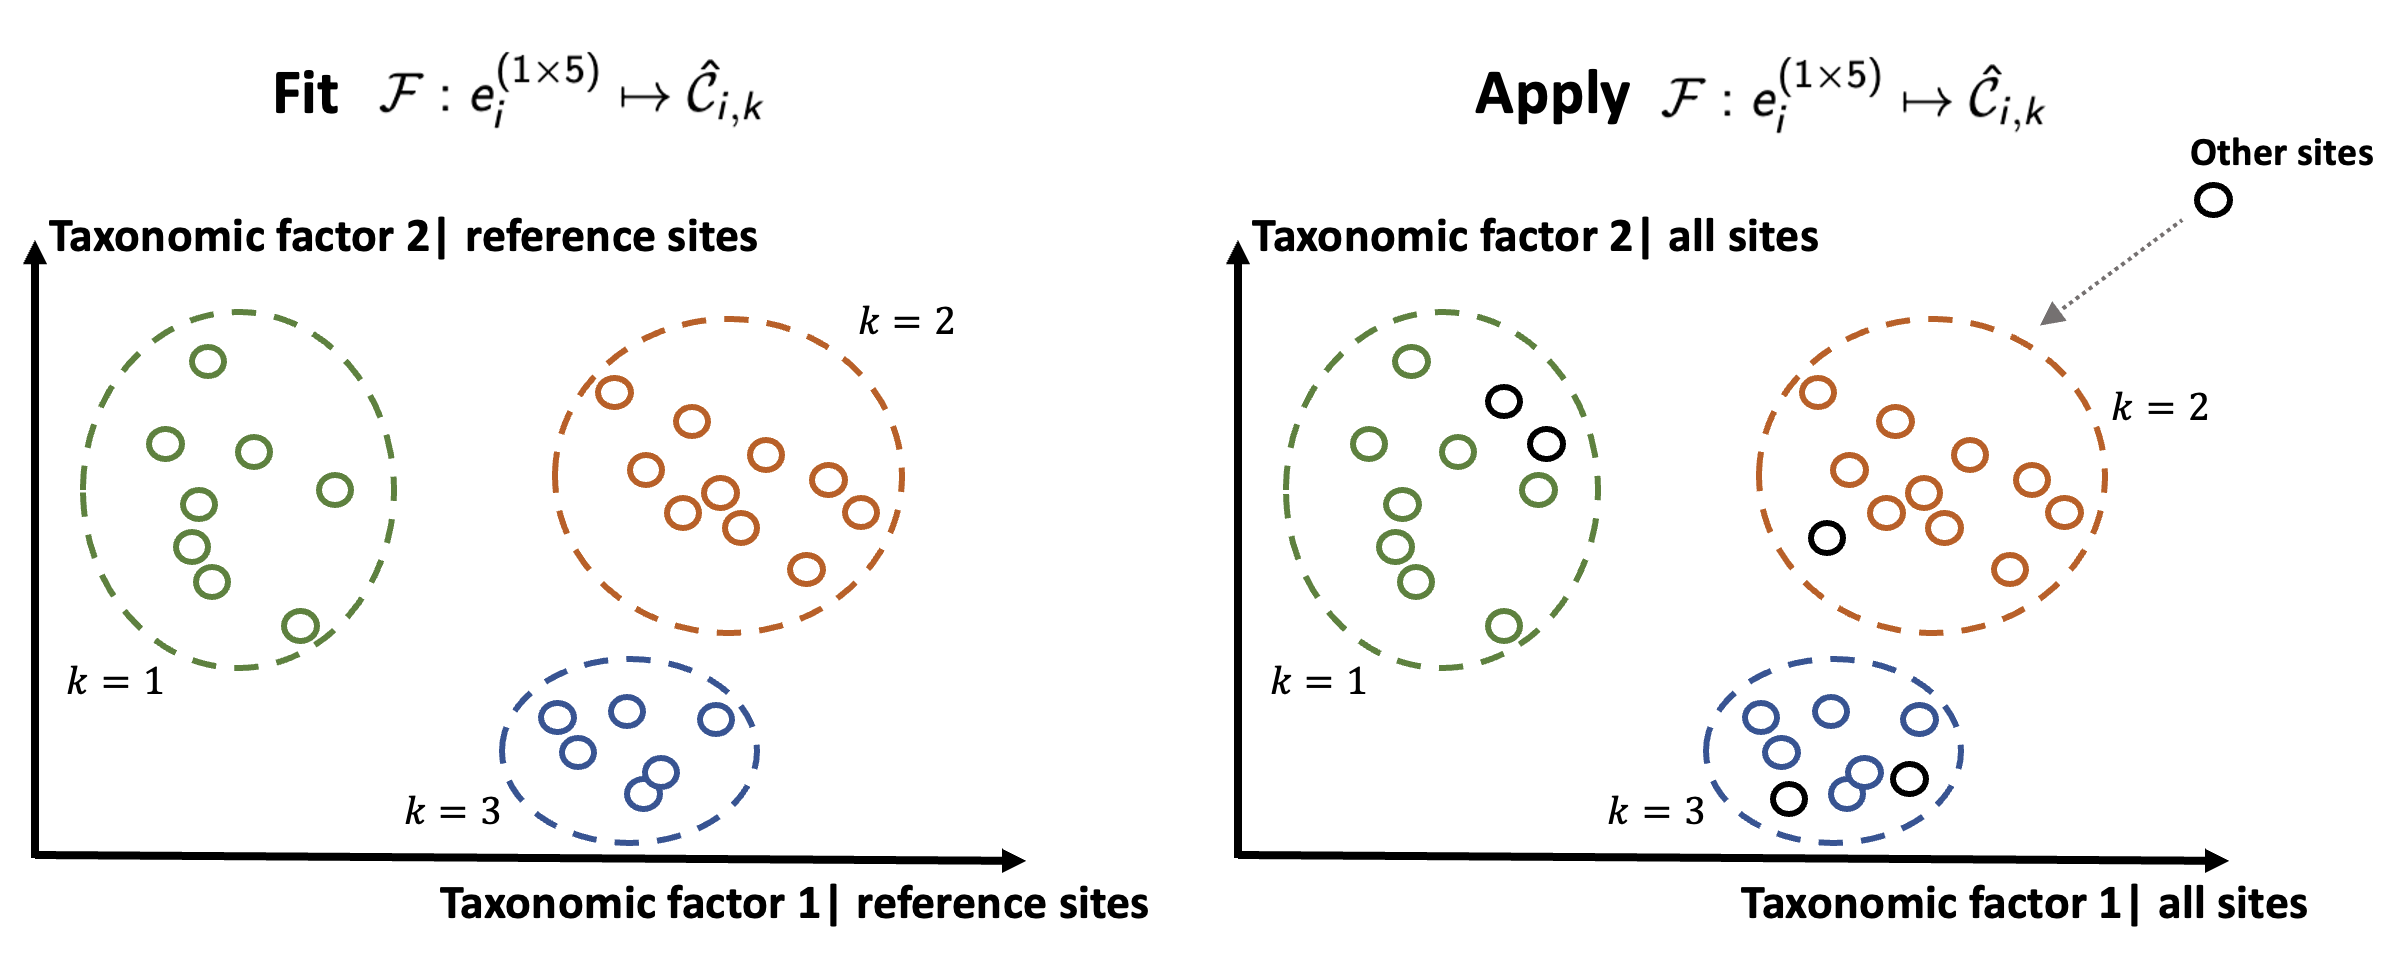
\includegraphics[width=0.8\textwidth]{../presentation/figures/p12_fit_apply_discriminant_function.png}
\caption{\textit{Visualization of the fitting and application of the discriminant function that assigns disturbed sites to the environmentally determined taxa composition groups.
}}
\label{fig:p12_fit_apply_discriminant_function}
\end{figure}

\subsection{Measure the difference from “pristine” to “true” taxa composition - Multivariate Gaussian Deviation Index }

\begin{figure}[!h]
    \centering
    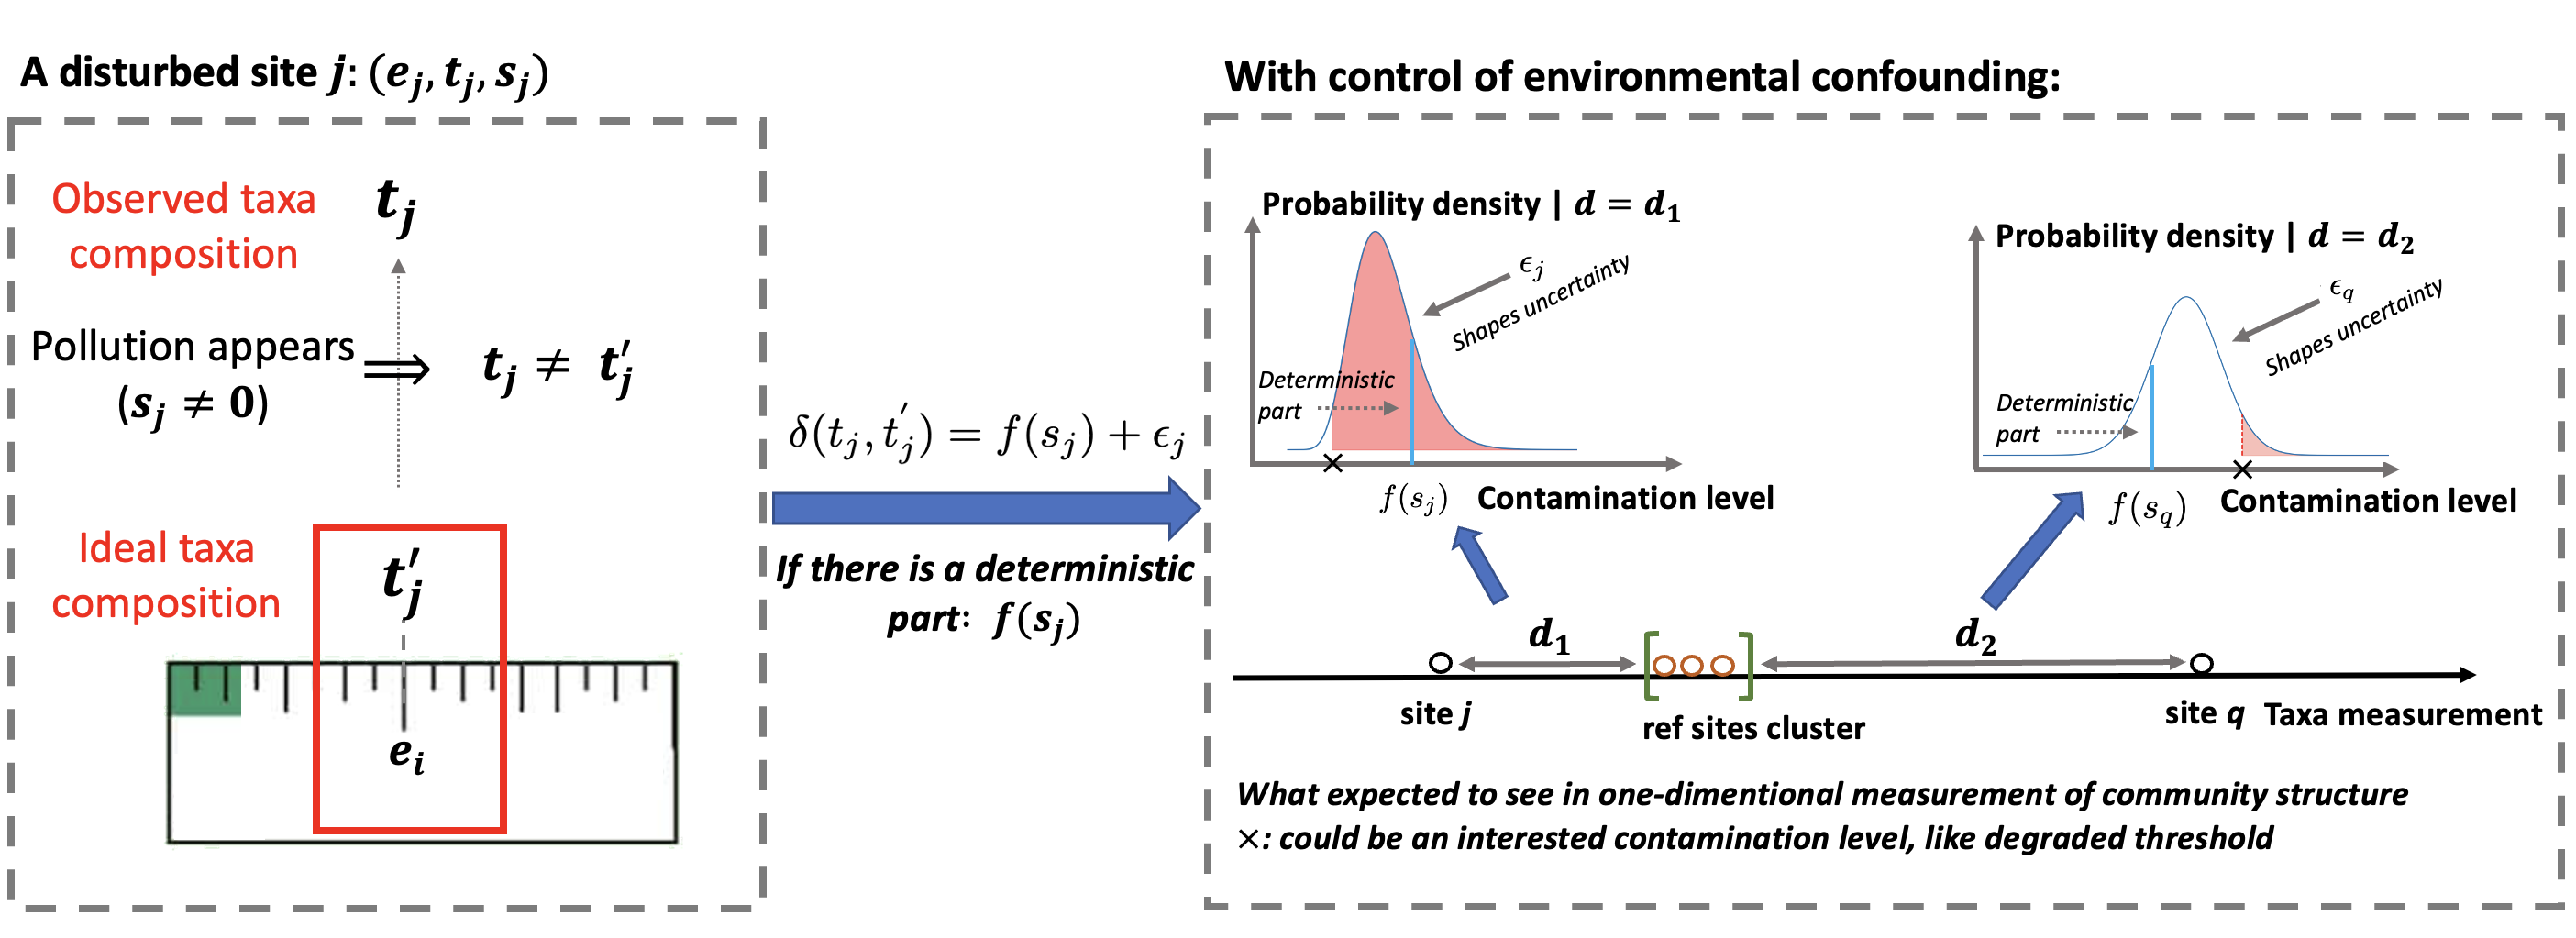
\includegraphics[width=0.8\textwidth]{../results/ideas_visualization/mark_taxa_difference_and_explain.png}
    \caption{\textit{The difference in taxa composition between the observed($t_{j}$) and ruler measured($t^{'}_{j}$) is connected to the sediment contamination level($s$).}}
    \label{fig:mark_taxa_difference_and_explain}
\end{figure}

Within each taxa-composition group $\mathcal{C}_k$, let $\mathcal{R}_k$ denote the set of reference sites ($I_{\text{ref}}=1$) and $\mathcal{D}_k$ the set of disturbed sites ($I_{\text{ref}}=0$).
We construct a site-level deviation metric that quantifies how far a site's observed community is from the pristine expectation of its group while controlling for environmental setting via $\mathcal{C}_k$.

% \paragraph{Choice of scale for community data.}
Because taxa compositions are multivariate and often compositional/zero-inflated, 
we first work on a transformed scale using the Hellinger transformation:
\[
\phi_{\mathrm{Hel}}:\;\mathbb{R}^{16}_{\ge 0}\rightarrow\mathbb{R}^{16}, \quad
\phi_{\mathrm{Hel}}(\mathbf{t})=
\left(
\sqrt{\frac{t^{(1)}}{\sum_{\ell=1}^{16} t^{(\ell)}}},\;
\dots,\;
\sqrt{\frac{t^{(16)}}{\sum_{\ell=1}^{16} t^{(\ell)}}}
\right).
\]
This transformation converts each taxon abundance to the square root of its relative abundance, 
reducing the influence of highly dominant taxa while preserving ecological distance relationships.
All subsequent quantities are computed on $\phi_{\mathrm{Hel}}(T)$; 
to simplify notation we overwrite $T \leftarrow \phi_{\mathrm{Hel}}(T)$.

There are other transformations that may be preferred depending on the context (e.g., log-ratio transforms, or raw counts),
the Hellinger transformation is tentative and can be replaced as needed.


After the transformation, for group $k$, compute the reference centroid and covariance
\[
\boldsymbol{\mu}_k \;=\; \frac{1}{|\mathcal{R}_k|}\sum_{i\in\mathcal{R}_k} T_{i}, 
\qquad
\boldsymbol{\Sigma}_k \;=\; \mathrm{Cov}\{T_{i}: i\in\mathcal{R}_k\} + \lambda I_{16},
\]
where $\lambda>0$ is a small ridge term to ensure invertibility and numerical stability, and 
$I_{16}$ is the $16\times 16$ identity matrix.
These parameters $(\boldsymbol{\mu}_k,\boldsymbol{\Sigma}_k)$ define a 
multivariate Gaussian-like distribution in the $16$-dimensional taxa space, representing the 
\emph{pristine community cloud} for group $k$.
Under this view, each reference site is a draw from 
$\mathcal{N}(\boldsymbol{\mu}_k, \boldsymbol{\Sigma}_k)$, 
and the geometric shape of this cloud is an ellipsoid whose orientation and size are determined by 
$\boldsymbol{\Sigma}_k$.

\subsubsection{Value-based Measurement: Z-score Community Index (ZCI)}
For any site $j$ in group $k$ (reference or disturbed), define the multivariate standardized 
deviation from the pristine centroid as the Mahalanobis distance:
\[
\mathrm{ZCI}_{k,j} \;=\; \sqrt{\big(T_{j}-\boldsymbol{\mu}_k\big)^{\top}\,\boldsymbol{\Sigma}_k^{-1}\,\big(T_{j}-\boldsymbol{\mu}_k\big)}.
\]
This measures how far $T_j$ lies from the center of the pristine Gaussian cloud, in units that 
account for both taxon-specific variability and cross-taxon correlations.
It effectively reduces the $16$-dimensional deviation vector to a \emph{single scalar score} 
while preserving the anisotropic geometry of the reference distribution.

When a diagonal approximation is preferred, use the ``sum of squared z-scores'' variant:
\[
\mathrm{ZCI}^{(\mathrm{diag})}_{k,j} \;=\; \sqrt{\sum_{\ell=1}^{16}\left(\frac{T^{(\ell)}_{j}-\mu^{(\ell)}_{k}}{\sigma^{(\ell)}_{k}}\right)^{2}},
\]
where $\sigma^{(\ell)}_{k}$ is the reference standard deviation of taxon $\ell$ in group $k$ 
(robust alternatives such as median absolute deviation may also be used).
This ignores inter-taxon correlations, treating the pristine cloud as an axis-aligned hypersphere, 
which can be more stable when the number of reference sites is small relative to the number of taxa.

\begin{figure}[!h]
\centering
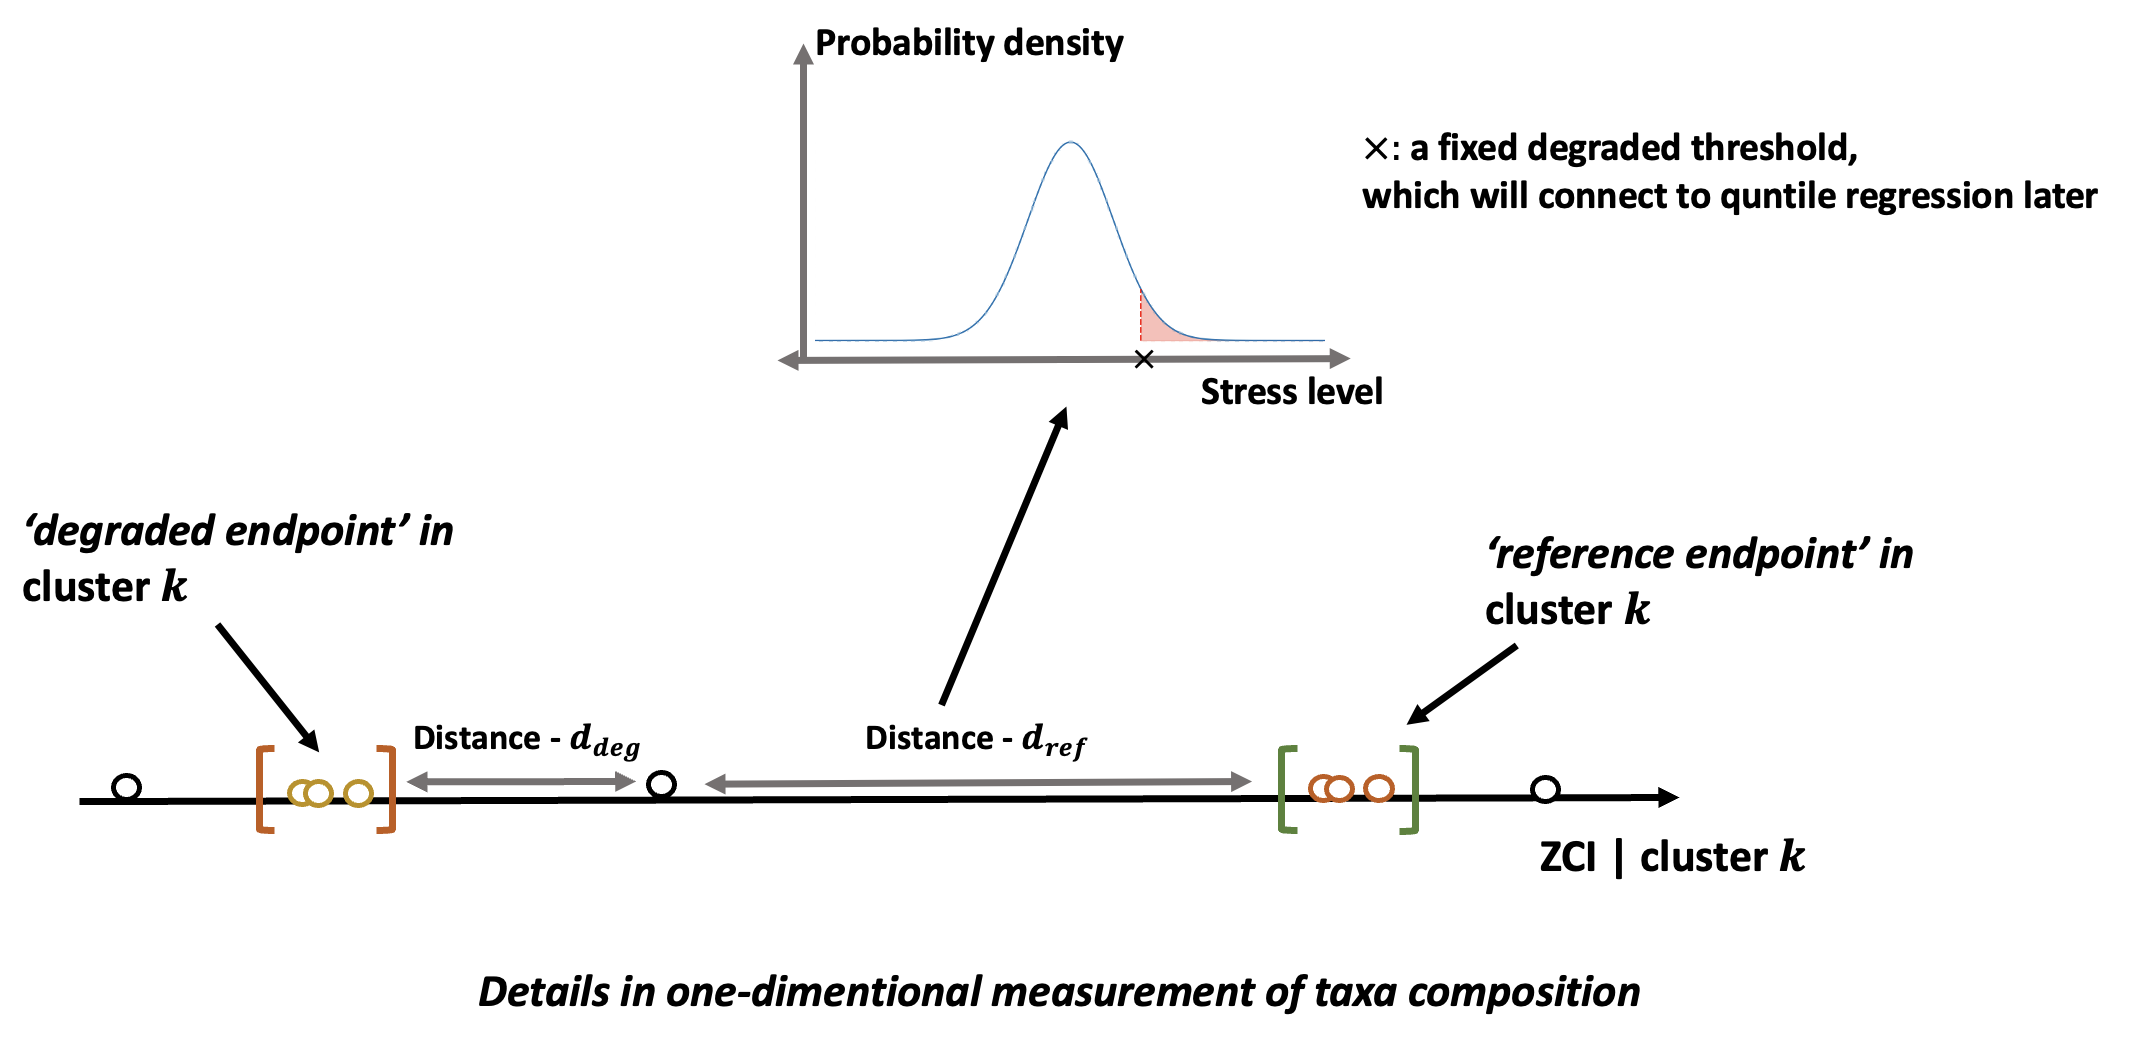
\includegraphics[width=0.8\textwidth]{../presentation/figures/p15_details_of_taxa_difference_in_1dimention.png}
\caption{\textit{Visualization of the details of taxa community structure differences measured in one-dimensional ZCI.}}
\label{fig:p15_details_of_taxa_difference_in_1dimention}
\end{figure}

\subsubsection{Vector-based Measurement: multi-dimensional ZCI}
The scalar $\mathrm{ZCI}_{k,j}$ summarizes deviation magnitude but discards the 
\emph{direction} of change in community composition.  
To retain more structure, the same Gaussian framework can be used to construct a 
multi-dimensional ZCI:

\begin{enumerate}
    \item \textbf{Whitening of deviations
    \footnote{Whitening means: Centering (subtracting \(\mu_k\)), rescaling and rotating so that the reference
    covariance becomes the identity matrix. Knowing that \(\Sigma_k = \frac{1}{|T|-1} (T - \mu)^T (T - \mu)\),
    replacing the \(T\) with \(\tilde{T} = \Sigma_k^{-1/2} (T - \mu)\),
    the new covariance matrix \(\tilde \Sigma_k\) becomes \(\frac{1}{|\tilde T| - 1} (\tilde{T} - \tilde \mu)^T (\tilde{T} - \tilde \mu) = I \) 
    . Here, \(T\) and \(\mu\) are both matrices and \(\Sigma_k\) is a non-singular matrix.}
    :} For each site $j$ in group $k$, compute the whitened deviation vector
    \[
    \tilde{T}_{k,j} = \boldsymbol{\Sigma}_k^{-1/2} (T_j - \boldsymbol{\mu}_k),
    \]
    where $\boldsymbol{\mu}_k$ and $\boldsymbol{\Sigma}_k$ are estimated from the reference sites.  
    Denote the matrix of whitened deviations for \emph{reference} sites as 
    $\tilde{T}_{k,\mathrm{ref}} \in \mathbb{R}^{n_{\mathrm{ref},k} \times 16}$.  
    In this whitened space, the reference cloud is isotropic and centered at the origin.
    
    \item \textbf{PCA fitted on whitened reference sites:}  
    Perform principal component analysis (PCA) on $\tilde{T}_{k,\mathrm{ref}}$ to obtain the loading matrix $V_k$.  
    Retain the first $d$ principal axes $V_{k,(1:d)}$, where $d=2$ gives a two-dimensional ZCI.

    \item \textbf{PCA applied to disturbed sites:}  
    For each disturbed site $j$, compute its whitened deviation $\tilde{T}_{k,j}$ using the \emph{same} $\boldsymbol{\mu}_k$ and $\boldsymbol{\Sigma}_k^{-1/2}$ from the reference sites, and project it onto the retained principal axes:
    \[
    \big( \mathrm{ZCI}^{(1)}_{k,j}, \mathrm{ZCI}^{(2)}_{k,j} \big)
    = \tilde{T}_{k,j} \; V_{k,(1:2)}.
    \]
\end{enumerate}

These coordinates preserve both magnitude and orientation of deviation in the most informative 
subspace of the pristine community cloud, enabling more nuanced comparisons between sites 
that have similar scalar ZCI values but differ in the \emph{type} of community shift.  
The scalar $\mathrm{ZCI}_{k,j}$ can be recovered as the Euclidean norm of these coordinates.

\begin{figure}[!h]
\centering
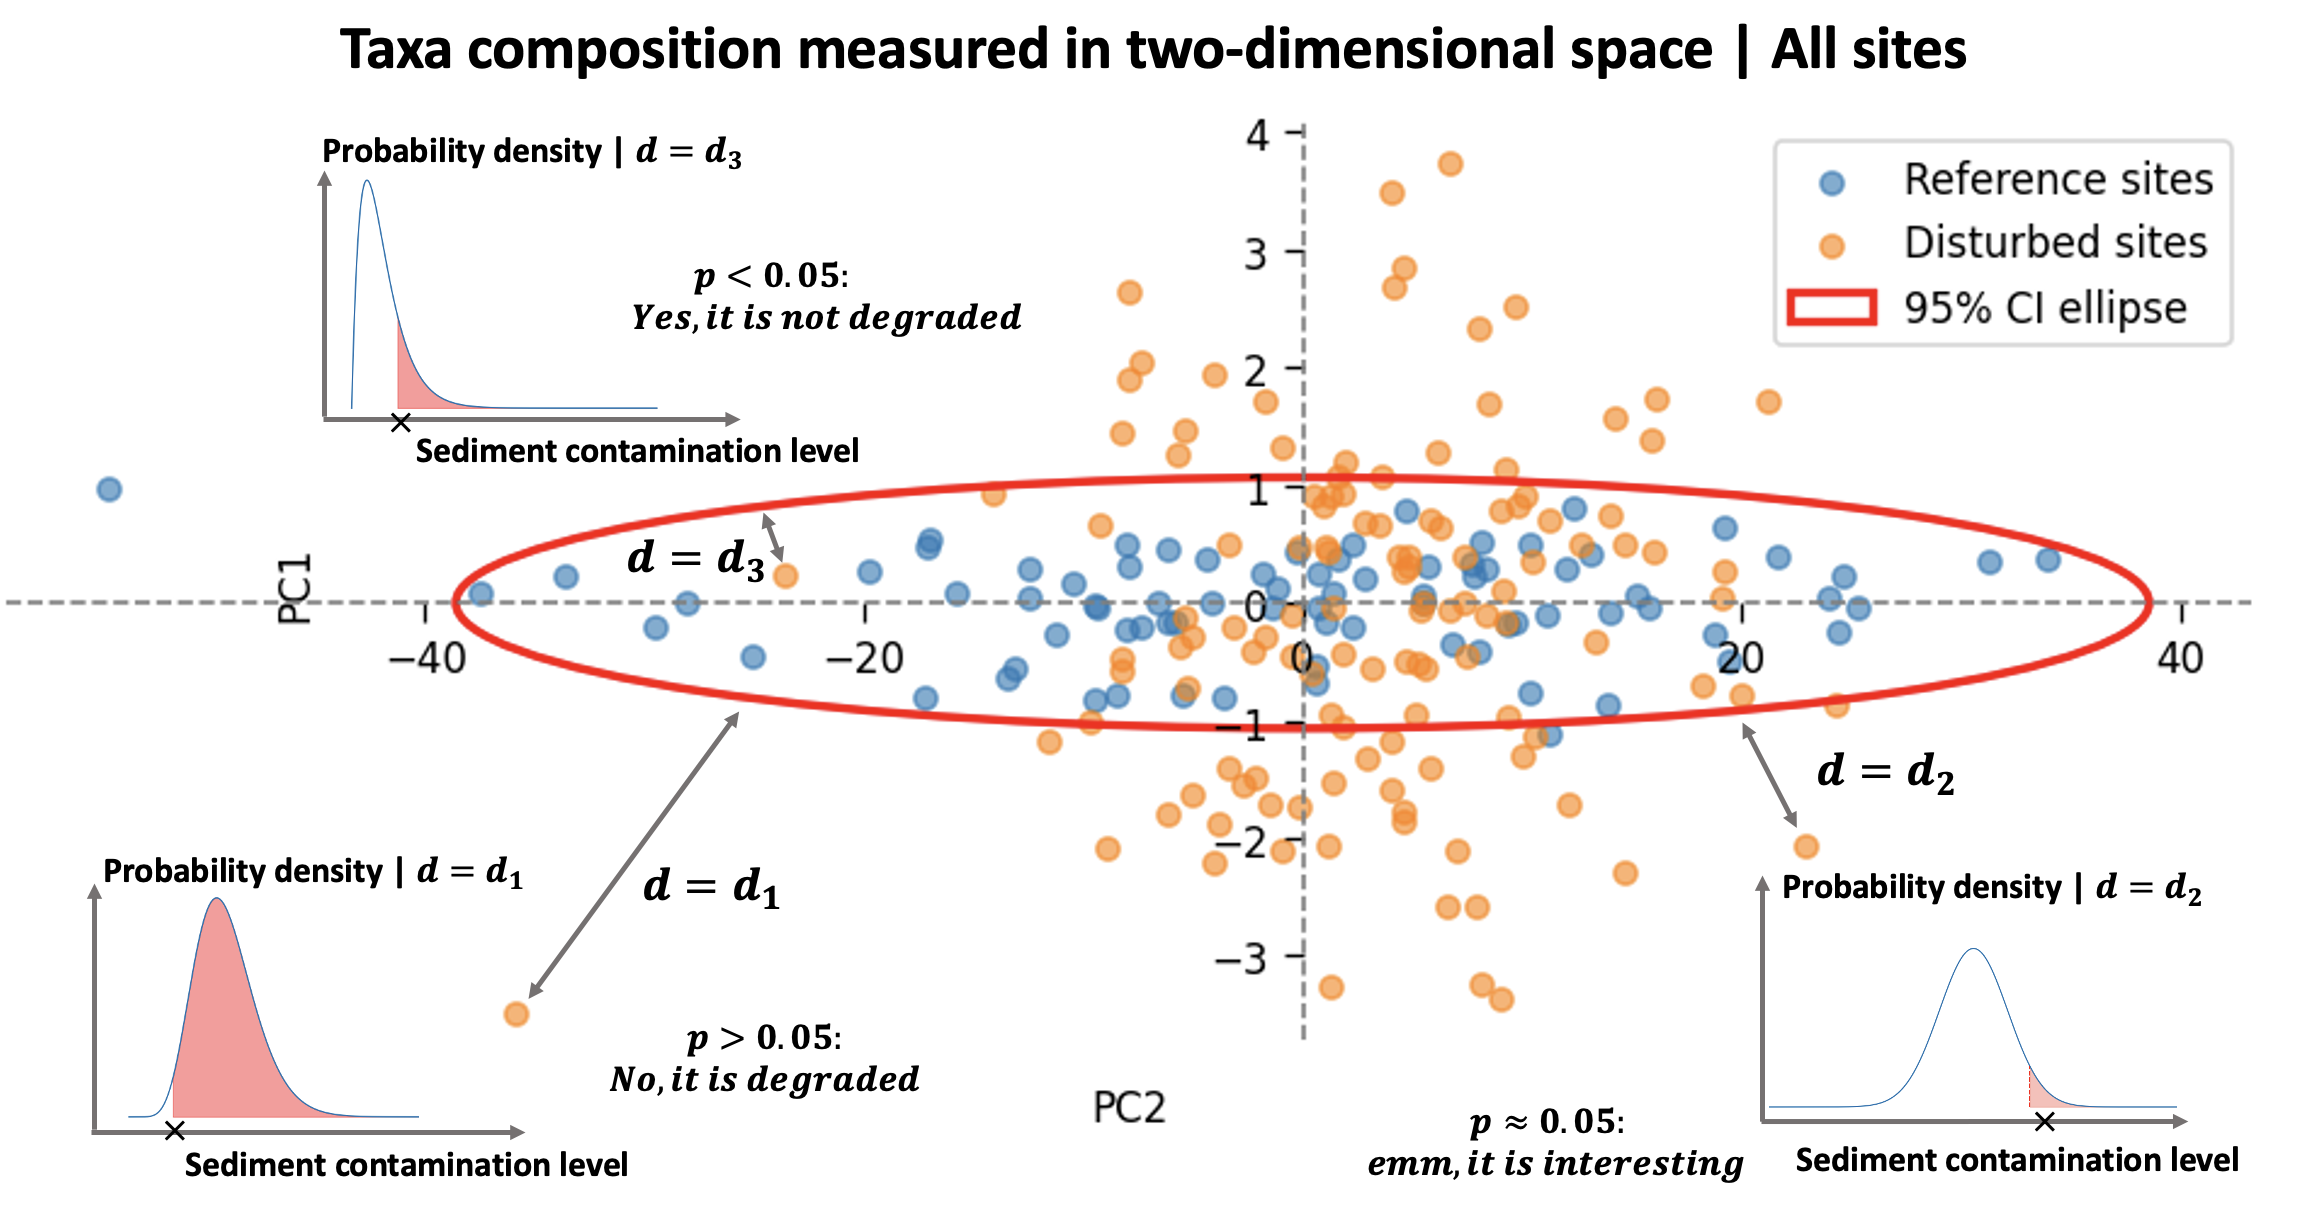
\includegraphics[width=0.8\textwidth]{../presentation/figures/p18_all_sites_in_2dimensional.png}
\caption{\textit{Visualization of the details of taxa community structure differences measured in two-dimension ZCI.}}
\label{fig:p18_all_sites_in_2dimensional}
\end{figure}

\subsubsection{Direction, interpretation, and optional 0--100 scaling.}

By construction, smaller values indicate communities closer to the pristine expectation for their environment; larger values indicate stronger deviation (putative impact).
For reporting, we optionally map ZCI to a condition scale where larger is better:
\[
\mathrm{ZCI}^{\star}_{k,j} \;=\; 100\,\big(1-\widehat{F}_k(\mathrm{ZCI}_{k,j})\big),
\]
with $\widehat{F}_k$ the empirical CDF of $\mathrm{ZCI}$ computed from \emph{reference} sites in group $k$. 
Under this calibration, reference sites cluster near higher scores (closer to $100$), while progressively disturbed sites trend toward $0$.

\subsection{Principal Coordinates of Neighbour Matrices (PCNM) for spatial eigenvectors}

To adjust the ZCI--stress relationships for residual spatial structure,
we derive spatial eigenvectors (PCNM variables) that capture multi-scale spatial autocorrelation
among the same set of $m$ sites in a specific cluster. 
These act as candidate covariates prior to fitting the piecewise quantile regression model.

Let $(x_j,y_j)$ be the planar (or projected) coordinates for site $j=1,\dots,m$.
Let $\mathbf{1}$ be an $m$-vector of ones, $\mathbf{I}_m$ the $m\times m$ identity, 
and the centering matrix $\mathbf{J}=\mathbf{I}_m-\tfrac{1}{m}\mathbf{1}\mathbf{1}^T$.

To derive spatial eigenvectors, we first compute Euclidean (or hydrologic, if river network) 
distances to form the $m\times m$ distance matrix $\mathbf{D}$ with entries:
\[
D_{ij}=\sqrt{(x_i-x_j)^2+(y_i-y_j)^2}
\]

Next, we choose a connectivity threshold $d_0$ as the maximum edge length of the minimum spanning tree to ensure a connected neighbour graph. Alternative approaches include using the maximum nearest-neighbour distance.

We then construct a truncated distance matrix $\mathbf{T}$ by defining 
\[
T_{ij} = \begin{cases}
D_{ij} & \text{if } D_{ij} \le d_0 \\
4d_0 & \text{otherwise}
\end{cases}
\]

where the large constant enforces separation of non-neighbours. 

The PCoA transform is applied by forming $\mathbf{A} = -\tfrac{1}{2}\,\mathbf{J}\,\mathbf{T}^{\circ 2}\,\mathbf{J}$ (where $^{\circ 2}$ denotes elementwise square), followed by eigen-decomposition $\mathbf{A}=\mathbf{V}\boldsymbol{\Lambda}\mathbf{V}^T$ with eigenvalues $\lambda_1\ge\cdots\ge\lambda_m$ and eigenvectors $\mathbf{v}_k$.
\[
\mathbf{A} = -\tfrac{1}{2}\,\mathbf{J}\,\mathbf{T}^{\circ 2}\,\mathbf{J} = \mathbf{V}\boldsymbol{\Lambda}\mathbf{V}^T, \quad
\]

We retain eigenvectors with positive eigenvalues $\lambda_k>0$ and 
scale them as $\mathbf{s}_k=\mathbf{v}_k\sqrt{\lambda_k}$. 
These orthogonal PCNM vectors span spatial patterns from broad (large $\lambda_k$) 
to fine scales. For screening, we compute Moran's $I$ for each $\mathbf{s}_k$ 
using a binary (or inverse-distance) weight matrix based on $d_0$, 
retaining only spatially autocorrelated vectors using FDR or adjusted $p$-values.
 Forward selection based on AIC or adjusted $R^2$ can be applied to avoid overfitting.

Finally, we collect the retained spatial vectors in $\mathbf{S}_{\text{sel}}\in\mathbb{R}^{m\times q_s}$ and add these to subsequent ZCI quantile regression models (using the same $\mathbf{S}_{\text{sel}}$ across $\tau$ for comparability). We test residual Moran's $I$ and iterate if needed.

% The retained PCNM set provides an orthogonal spatial basis approximating latent spatial processes not captured by measured environmental variables. Incorporating $\mathbf{S}_{\text{sel}}$ isolates the anthropogenic (contamination) signal in ZCI–stress relationships, reducing bias and inflated Type I error from spatial autocorrelation. Resulting variation partitioning can then attribute explained variance uniquely to contamination versus spatial structure.




\subsection{Build ZCI indicator of sediment contamination levels – Piecewise Quantile Regression Model}

The $\mathrm{ZCI}$ score reflects the degree of deviation in taxa composition from the pristine expectation within each group $k$, given the same environmental context. 
Because both the stress level and the community condition are influenced by a range of measured and unmeasured factors, it is reasonable to model the conditional distribution of the stress level \emph{given} the community departure.  
This regression is used only as a statistical association to infer likely stress levels from observed $\mathrm{ZCI}$ values and does \textbf{not} imply a causal relationship between stress and community departure.

Within each group \(k\), we relate the relative stress level to the ZCI deviation \emph{and} the selected spatial eigenvector predictors derived earlier. Let
\[
z_{k,j}:=\mathrm{ZCI}_{k,j}, \qquad \mathbf{s}_{k,j}\in\mathbb{R}^{q_s}\text{ be row }j\text{ of }\mathbf{S}_{\text{sel}} (q_s \text{ retained PCNM vectors}).
\]
We model
\[
\delta X_{k,j} = \mathcal{F}_{k}\big(z_{k,j},\,\mathbf{s}_{k,j}\big)+\varepsilon_{k,j},
\]
where $\delta X_{k,j}$ is the relative stress (e.g., $s_j-\mathrm{median}\{s_i:i\in\mathcal{R}_k\}$). Using the \emph{same} spatial basis $\mathbf{S}_{\text{sel}}$ across all quantiles $\tau$ preserves comparability of slope and breakpoint inference by ensuring spatial adjustment does not vary with $\tau$.

Given potential nonlinearity in $z$ and heteroscedasticity, we use a piecewise linear quantile formulation in $z$ while treating spatial terms additively:
\[
Q_{\delta X\mid Z,S}^{(k)}(\tau \mid z, \mathbf{s}) = f_{k,\tau}(z,\mathbf{s}) = \beta_{0,\tau}^{(k)} + \beta_{1,\tau}^{(k)} z + \sum_{m=1}^{M} \gamma_{m,\tau}^{(k)} (z-\kappa_m)_+ + \sum_{r=1}^{q_s} \alpha_{r,\tau}^{(k)} s^{(r)},
\]
with breakpoints $\kappa_1<\cdots<\kappa_M$ placed on the ZCI axis only (spatial covariates are not segmented). Parameters solve the check-loss minimization
\[
\widehat{\boldsymbol{\theta}}_{\tau}^{(k)} \in \arg\min_{\boldsymbol{\theta}} \sum_{j\in\mathcal{C}_k} \rho_{\tau}\Big( \delta X_{k,j} - f_{k,\tau}(z_{k,j},\mathbf{s}_{k,j}) \Big), \qquad \rho_{\tau}(u)=u\{\tau-\mathbf{1}(u<0)\}.
\]
The fitted conditional quantile surface is then
\[
\widehat{Q}_{\delta X\mid Z,S}^{(k)}(\tau \mid z,\mathbf{s}) = \widehat{\beta}_{0,\tau}^{(k)} + \widehat{\beta}_{1,\tau}^{(k)} z + \sum_{m=1}^{M} \widehat{\gamma}_{m,\tau}^{(k)} (z-\kappa_m)_+ + \sum_{r=1}^{q_s} \widehat{\alpha}_{r,\tau}^{(k)} s^{(r)}.
\]
Including the spatial term ensures that breakpoint and slope interpretations are attributed to contamination-driven community departure rather than residual spatial patterning.

\subsubsection{Hypothesis testing for degradation -- Quantile-based threshold inference}

In many applications, a binary classification of a site as ``degraded'' or ``non-degraded'' 
is more actionable than estimating its exact stress level. 
This decision problem can be formulated as a one-sided hypothesis test, conditioning on the 
observed community departure (ZCI):

\begin{itemize}
    \item \textbf{Step 1 -- Define degradation threshold.}  
    For each group $k$, choose a stress threshold $x_{k}^*$ 
    (e.g., a regulatory limit or an ecologically relevant benchmark) 
    that separates degraded from non-degraded sites.

    \item \textbf{Step 2 -- Predict conditional stress distribution.}  
    For a site $j$ with observed $\mathrm{ZCI}_{k,j}=z$, 
    use the fitted quantile regression model 
    ${Q}_{\delta X\mid Z,S}(\tau | z, \mathbf{s})$ over a grid of quantile levels 
    $\tau \in (0,1)$ to approximate the conditional distribution 
    $F_{\delta X\mid Z, S}^{(k)}(x | z, \mathbf{s})$. 
    This is done by inverting the quantile function across $\tau$.

    \item \textbf{Step 3 -- Compute $p$-value for degradation.}  
    The hypothesis test is:
    \[
    H_0: \delta X_{k,j} \le x_{k}^* \quad \text{vs.} \quad H_a: \delta X_{k,j} > x_{k}^* .
    \]
    The conditional $p$-value is then
    \[
    p = 1 - F_{\delta X\mid Z,S}^{(k)}\!\left( x_{k}^* \,\middle|\, z, \mathbf{s} \right),
    \]
    which represents the probability, given the site's ZCI and spatial context, that the stress level 
    exceeds the degradation threshold.
\end{itemize}

If $p$ is below a chosen significance level $\alpha$ (e.g., $0.05$), 
the site is classified as degraded; otherwise, it is classified as non-degraded.  
This approach converts the regression output into a probabilistic decision rule while 
controlling for environmental setting via the group-specific model.

\begin{figure}[!h]
\centering
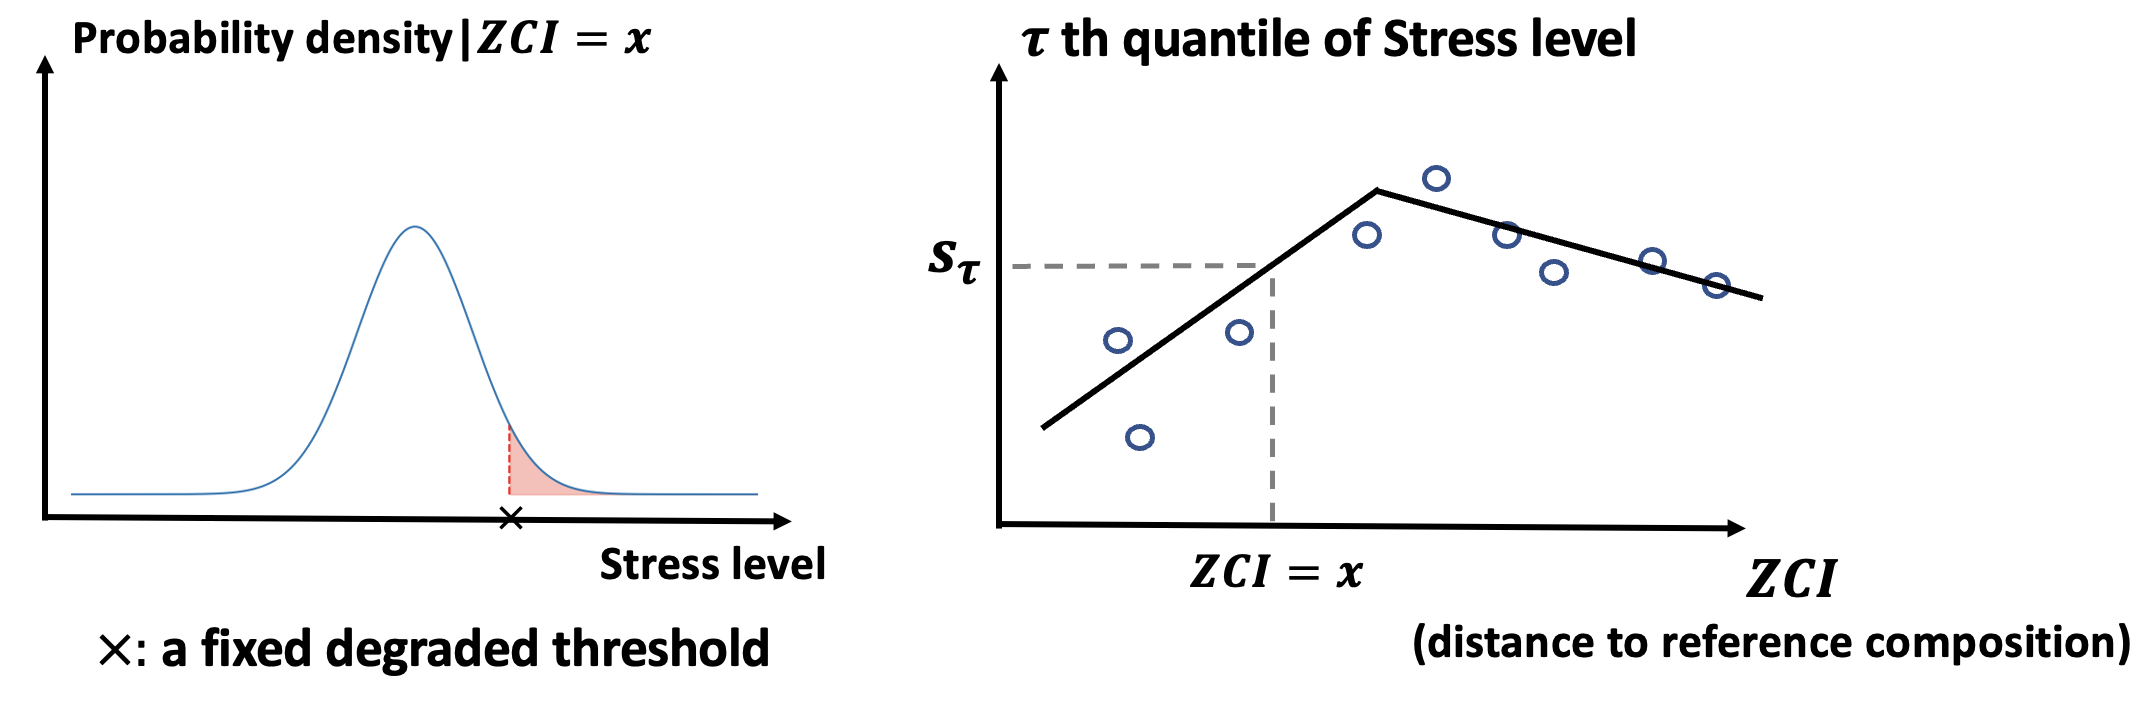
\includegraphics[width=0.9\textwidth]{../presentation/figures/p16_degraded_threshold_and_quantile_regression.png}
\caption{\textit{A pre-fixed degradation threshold on the conditional stress level distribution and the correspondingly predicted quantile value \(\hat s_{\tau}\)}}
\label{fig:p16_degraded_threshold_and_quantile_regression}
\end{figure}


\subsection{Indicator power and robustness with respect to sample size (tentative)}
Power and robustness evaluation of the indicator can be divided into the following specific aims: 
(i) quantify precision of slopes and breakpoint effects and conditional quantiles as sample size varies 
and (ii) estimate power for detecting contamination structure and degradation thresholds, all \emph{within each group $k$}.

	\textbf{Targets:} slopes $\beta_{1,\tau}^{(k)}$, changes $\gamma_{m,\tau}^{(k)}$, breakpoint reliability, pseudo-$R^2$, degradation test (Type I / power), and conditional quantiles $\widehat Q_{\delta X|Z,S}$.

	\textbf{Procedure (tentatively designed steps):}
\begin{enumerate}
    \item \emph{Baseline fit:} Fit full piecewise quantile model (fixed $\kappa_m$, fixed $S_{\text{sel}}$) for $\tau \in \mathcal{T}$; store parameters and residuals; test residual Moran's $I$.
    \item \emph{Bootstrap (uncertainty):} If no residual spatial autocorrelation: site bootstrap; else block bootstrap. Refit using original $S_{\text{sel}}$; derive percentile CIs and relative widths.
    \item \emph{Subsampling (precision curves):} For a grid of reduced sizes $n_k^{(g)}$, draw $R$ subsamples preserving 
    ratio of \(\frac{reference}{disturbed}\); refit; summarize bias and RMSE of slopes / predicted quantiles; locate diminishing returns size.
    % \item \emph{Effective sample size:} When mild spatial correlation persists, report $ n_{k,\text{eff}} = \dfrac{n_k}{1 + (n_k-1)\bar{\rho}_k }$ and inflate SEs by $\sqrt{n_k/n_{k,\text{eff}}}$.
    \item \emph{Power simulation:} \(H_0\): $\beta_{1,\tau}=\gamma_{m,\tau}=0$; \(H_1\): baseline (and reduced effect). Simulate $L$ datasets holding $(z, S_{\text{sel}})$ fixed; estimate power for joint slope/breakpoint test and degradation classification at threshold $x_k^*$.
    \item \emph{Breakpoint reliability:} Accept $\kappa_m$ if CI width $< 0.3$ of ZCI span \emph{and} $\Pr(\gamma_{m,\tau}\neq 0 \text{ for some } \tau) \ge 0.8$; otherwise reduce segments or increase sample size.
    \item \emph{Outputs:} (a) precision and power curves vs. $n_k$; (b) recommended minimum $n_k$ meeting power $\ge 0.8$ (median quantile) and reliability rule; (c) table of median (IQR) parameter estimates.
\end{enumerate}

	\textbf{Interpretation:} Early plateau in precision implies reallocating effort to under-sampled groups or spatial gaps.
     If slopes are consistent but breakpoints unreliable, report continuous gradients instead of thresholds.
    Reliable, sharp breakpoints support categorical management triggers.


\section{Preliminary exploration}

In this section, I implemented a simplified completed workflow based 
on the methodology described in Section Methodology. 
It explored the practical application of the proposed method to support the later composite workflow.
Specifically, the major preliminary steps are as follows:

\begin{enumerate}

\item \textbf{Collect comparable data.}

There are three available datasets, containing the three raw data types: zoobenthic community data (311×16), chemical data (104×30), and environmental data (289×7).
The three shared the same identical index - StationID, which supports data merging to prepare completed data for 
each site. After merging there is a combined dataset with 104 rows and 53 columns, containing all three types of data.

\textbf{Key Results:} \(\left[
\begin{array}{ccc}
X & E & T
\end{array}
\right]
\in
\mathbb{R}^{m \times (30 + 5 + 16)}\) was prepared
\footnote{
The column numbers were not consistent(\(51 \neq 53\))
because StationID and location information were not used in the analysis.
Later, the location information can be included to support spatial analysis.
}.

\item \textbf{Assess sediment contamination and Identify reference and degraded sites.}

A log-transformation was applied to the chemical data to reduce dominance by high-value variables.
Then PCA was performed on the transformed chemical data and several principal components were selected to explain
the major variation of pollutant elements. By simply standardizing and summing these PCs, comprehensive stress values were computed for each site.
To keep consistency with Jian's analysis, I used the name "SumReal" to refer these stress values (levels).
Current statistics results shown "the higher are the stress scores, the less are the pollutant elements concentrations",
but this will be further explored in the future.

Based on the computed stress scores,  \(p\%\) was temporarily set to 20\% to identify reference sites and the degraded sites were symmetrically defined.
Out of assumption, there were no or minimal human disturbances on the reference sites, their taxa composition was shaped by environmental conditions only.


\textbf{Key Results:} \(\left[
\begin{array}{ccccc}
X & E & T & s & I_{ref}
\end{array}
\right]
\in
\mathbb{R}^{m \times (51 + 2)}\), \(\) was prepared

\item \textbf{Cluster reference sites by taxa community composition.}

Turn to the zoobenthic community data of these references, IQR method was applied to detect outliers
and then octave transformation was applied to reduce extreme values' impact, 
considering that taxa in low abundance do not mean they are not important.

Then clustering was applied to identify major taxa community patterns across different environmental conditions,
and \(K\) clusters were identified. Here \(K\) was set to 3 through the hierarchical clustering method.
These sites assigned into each \(k\) cluster represent "ideal" taxa structures,
each totally shaped by the range of environmental conditions of the corresponding cluster.

\textbf{Key Results:} 
\(\mathcal{C}_K\)
and
\(\left[
\begin{array}{cccccc}
X & E & T & s & I_{ref} & \mathcal{C}_K
\end{array}
\right]_{I_{ref} = 1}
\in
\mathbb{R}^{(p\% \times m) \times (53 + 1)}\), were prepared.

\item \textbf{Fit Discriminant Function of environmental factors for taxa clusters.}

Based on the identified clusters of these reference sites,
a discriminant function was fitted to predict the taxa cluster membership of each site based on its environmental variables.
\footnote{It is both acceptable to say "environmental clusters" or "taxa clusters", owing to the assumption that 
these reference sites have their taxa composition totally shaped by the environmental conditions.} 

\textbf{Key Results:} 
\(\mathcal{F}_{dis}: e^{(1, 5)} \to \hat C_K\) was fitted.

\item \textbf{Apply the Discriminant Function to rest disturbed sites to group them}

To the (1 - \(p\%\)) disturbed sites, including the degraded sites, 
\(\mathcal{F}_{dis}\) was applied to assign each site to one of the identified taxa clusters.

\textbf{Key Results:} 
\(\mathcal{F}_{dis}: e^{(1, 5)} \to \hat C_K\) was applied, 
\(\left[
\begin{array}{cccccc}
X & E & T & s & I_{ref} & \mathcal{\hat C}_K
\end{array}
\right]_{I_{ref} = 0}\) was prepared.

\item \textbf{Construct endpoints and compute ZCI in each cluster.}

Within each cluster, the reference sites and degraded sites were used to construct endpoints, 
unlike the Multivariate Gaussian cloud of reference sites, 
the endpoints were simply computed as the means of 3 selected references and 3 degraded sites.
The endpoints were used to numerically scale the taxa community structure and compute the Zoobenthic Condition Index via 
Bray-Curtis ordination method. The \(ZCI_{k}\) reflected the distance of the disturbed sites to the endpoints in cluster \(k\).

\textbf{Key Results:} 
\(ZCI_{k}, (k \in {1, ..., K})\) was computed; \(ZCI_{k, j}\) reflects the distance of site \(j\) to its cluster \(k\) endpoints.

\item \textbf{Evaluate the ZCI vs SumReal relationship by quantile regression.}

On top of the \(ZCI\) and stress level \(s\), a piecewise quantile regression was fitted to evaluate their relationship across 
the three taxa clusters. The breakpoints were found by grid search method with a pre-defined searching range, which 
was set manually based on the preliminary exploration.

\textbf{Key Results:} 
\(f_{k, \tau}(z), (k \in {1, ..., K})\) was fitted; \(\hat \theta_{\tau}^{(k)}\) was solved for each cluster \(k\).

\item \textbf{Preliminary exploration of spatial structure with simulation}

An isolated PCNM (spatial eigenfunction) simulation was run, separate from previous workflow steps, to illustrate extraction of spatial structure across increasing complexity. Three scenarios were simulated (low to higher complexity): (i) equally spaced 1D sites, (ii) equally spaced 2D lattice, and (iii) irregular 2D sites with two clusters. The first two yield regular distance matrices and smoothly ordered (broad- to fine-scale) eigenvectors; the clustered irregular layout produces wave-like spatial patterns in the leading eigenfunctions.

\textbf{Key Results:} \(PCNM: D \to S_{\text{sel}}\) was carried out; \(S_{\text{sel}}\) comprises the Moran's I–screened spatial eigenvectors derived from the truncated neighbour distance matrix \(D\).

\item \textbf{Power and sensitivity analysis on quantile regression with simulation}

A deterministic piecewise quantile regression model with fixed breakpoint \(\kappa\) and heteroscedastic noise was used to generate synthetic data. Subsamples of sizes \(n=20,50,80,\dots,500\) were drawn to assess estimation precision of key parameters (\(\hat y_{\tau}\), \(\beta_{1,\tau}\), \(\delta_{\tau}\)). Bootstrap 95\% CIs and precision curves (RMSE) were computed. Power analysis for detecting non-zero hinge effects (\(\delta\neq 0\)) was conducted via repeated simulation under alternative and null conditions.

\textbf{Key Results:} Preliminary patterns show (i) diminishing RMSE gains beyond moderate \(n\); (ii) wider CIs and reduced power at extreme quantiles; (iii) hinge (\(\delta_{\tau}\)) estimates stabilising more slowly than primary slope estimates. Several implementation and interpretation issues (e.g., behaviour at high \(\tau\) with small \(n\)) were noted for later, more detailed exploration.


\end{enumerate}

\input{sections/subsectionofPreliminaryResults.tex}
\clearpage
\section{Practical Implementation Plan}

This section outlines the specific implementation plan for the thesis project,
detailing the project structure, work patterns and the benefits of this approach.

The current project structure is designed into 9 major folders,
each with a specific storage function as briefly described in
Table \textcolor{blue}{\ref{tab:project_structure}}.

\begin{table}[!h]
\centering
\caption{Project folder structure and description}
\label{tab:project_structure}
\renewcommand{\arraystretch}{1.3}
\begin{tabular}{p{3cm}p{10cm}}
\hline
\textbf{Folder} & \textbf{Description} \\
\hline
\texttt{src/} & Core source code package (\texttt{ecoindex}) with reusable analysis modules. \\
\texttt{notebooks/} & Interactive Jupyter notebooks for prototyping and exploratory work that majorly achieves by modules from \textit{src}. \\
\texttt{tests/} & Unit tests for packages wrote in \texttt{ecoindex}, using \texttt{pytest} to ensure correctness and reliability. \\
\texttt{configs/} & Centralized configuration (random seeds, parameters, file paths),
collective containers for important parameters. \\
\texttt{data/} & Raw and processed datasets, organized for reproducibility. \\
\texttt{artifacts/} & Outputs not easily reproducible, e.g., trained models or serialized results. \\
\texttt{figures/} & Generated plots, charts, and visualizations for reporting. \\
\texttt{reference/} & External references, guidelines, and supporting documentation. \\
\texttt{documents/} & Thesis drafts, LaTeX files, lying close to results folders to keep
synchronous with the results.\\
\hline
\end{tabular}
\end{table}

The following two subsections will elaborate on the principles and rationales behind this project structure design,
and use a specific example to demonstrate the codebase design and working pattern.

\subsection{Research Professional Codebases}
To make a good research professional codebase, I want to follow the principles of modularity, reusability and maintainability.
This means organizing code into reusable components, documenting functionality clearly, 
doing tests for all components, and ensuring that the codebase can be easily understood and modified.

Out of these principles, the code structure and organization become paramount in achieving the work.
It has to be admitted that such structure would cost more time in setting up and analysing 
the meta data, significant amount of time when compared to directly writing the code in a single 
file. However, with the progress of the project, the benefits of this structure will become apparent
and obviously accelerate the research process, which is visible and achievable to
a non-computer science student with the support of these Generative AI tools.

The following example shows a quick starting point for the codebase, where I wrote
and wrote some functions to achieve a given data transformation operation, wrapping
it in a clear structured way into original data frame and testing the correctness 
of these operations. 

\subsubsection{Modularized Function implementation and lightweight application}

As it was mentioned in the methodology part, I wanted to continuously add computed 
results, which were sitewise specific, into the original data frame meanwhile
keeping the whole data frame tiny and efficient. Assuming I had the three raw data sets in my
\textit{data/raw} folder, and I wanted to do a hellinger transformation on the
taxa data set and export the transformed data into the \textit{data/processed} folder.
To achieve this complete operation, I would need the following modules and functions within them:

\begin{table}[!h]
\centering
\caption{Temporary Code Structure for Hellinger Transformation and Integrity of Data Frame}
\label{tab:module_structure}
\renewcommand{\arraystretch}{1.3}
\begin{tabular}{p{3.5cm}p{9.5cm}}
\hline
\textbf{Module} & \textbf{Description} \\
\hline
\textit{src/config.py} & Configuration management for centralized parameter storage and project settings,
like file paths and processing options. \\
\hline
\textit{src/cleaning.py} & Data cleaning utilities for handling missing values, outliers, and data quality issues. \\
\hline
\textit{src/ingest.py} & Data ingestion functions for loading raw datasets from various sources and formats. \\
\hline
% \textit{src/data-io.py} & Input/output operations for reading and writing data files in different formats. \\
% \hline
\textit{src/dataframe-ops.py} & DataFrame manipulation utilities for wrapping new information into layered data frames \\
\hline
\textit{src/transform.py} & Data transformation functions including ecological transformations like Hellinger. \\
\hline
\textit{src/pipeline.py} & Pipeline orchestration for chaining multiple data processing steps together. \\
\hline
\textit{notebooks/0-interim-data.py} & Notebook to invoke the above functions in practical scenarios,
lightweight code snippets for quick testing and validation. \\
\hline
\textit{tests/test-*.py} & Unit tests for validating the functionality of individual modules and functions
in above modules(\textit{src/*}). \\
\hline
\end{tabular}
\end{table}

The whole modules are not only designed for Hellinger Transformation, but it is a good example and there will be more
functions and module added in this structure to make the project concise and reproducible.

\begin{figure}[!h]
    \centering
    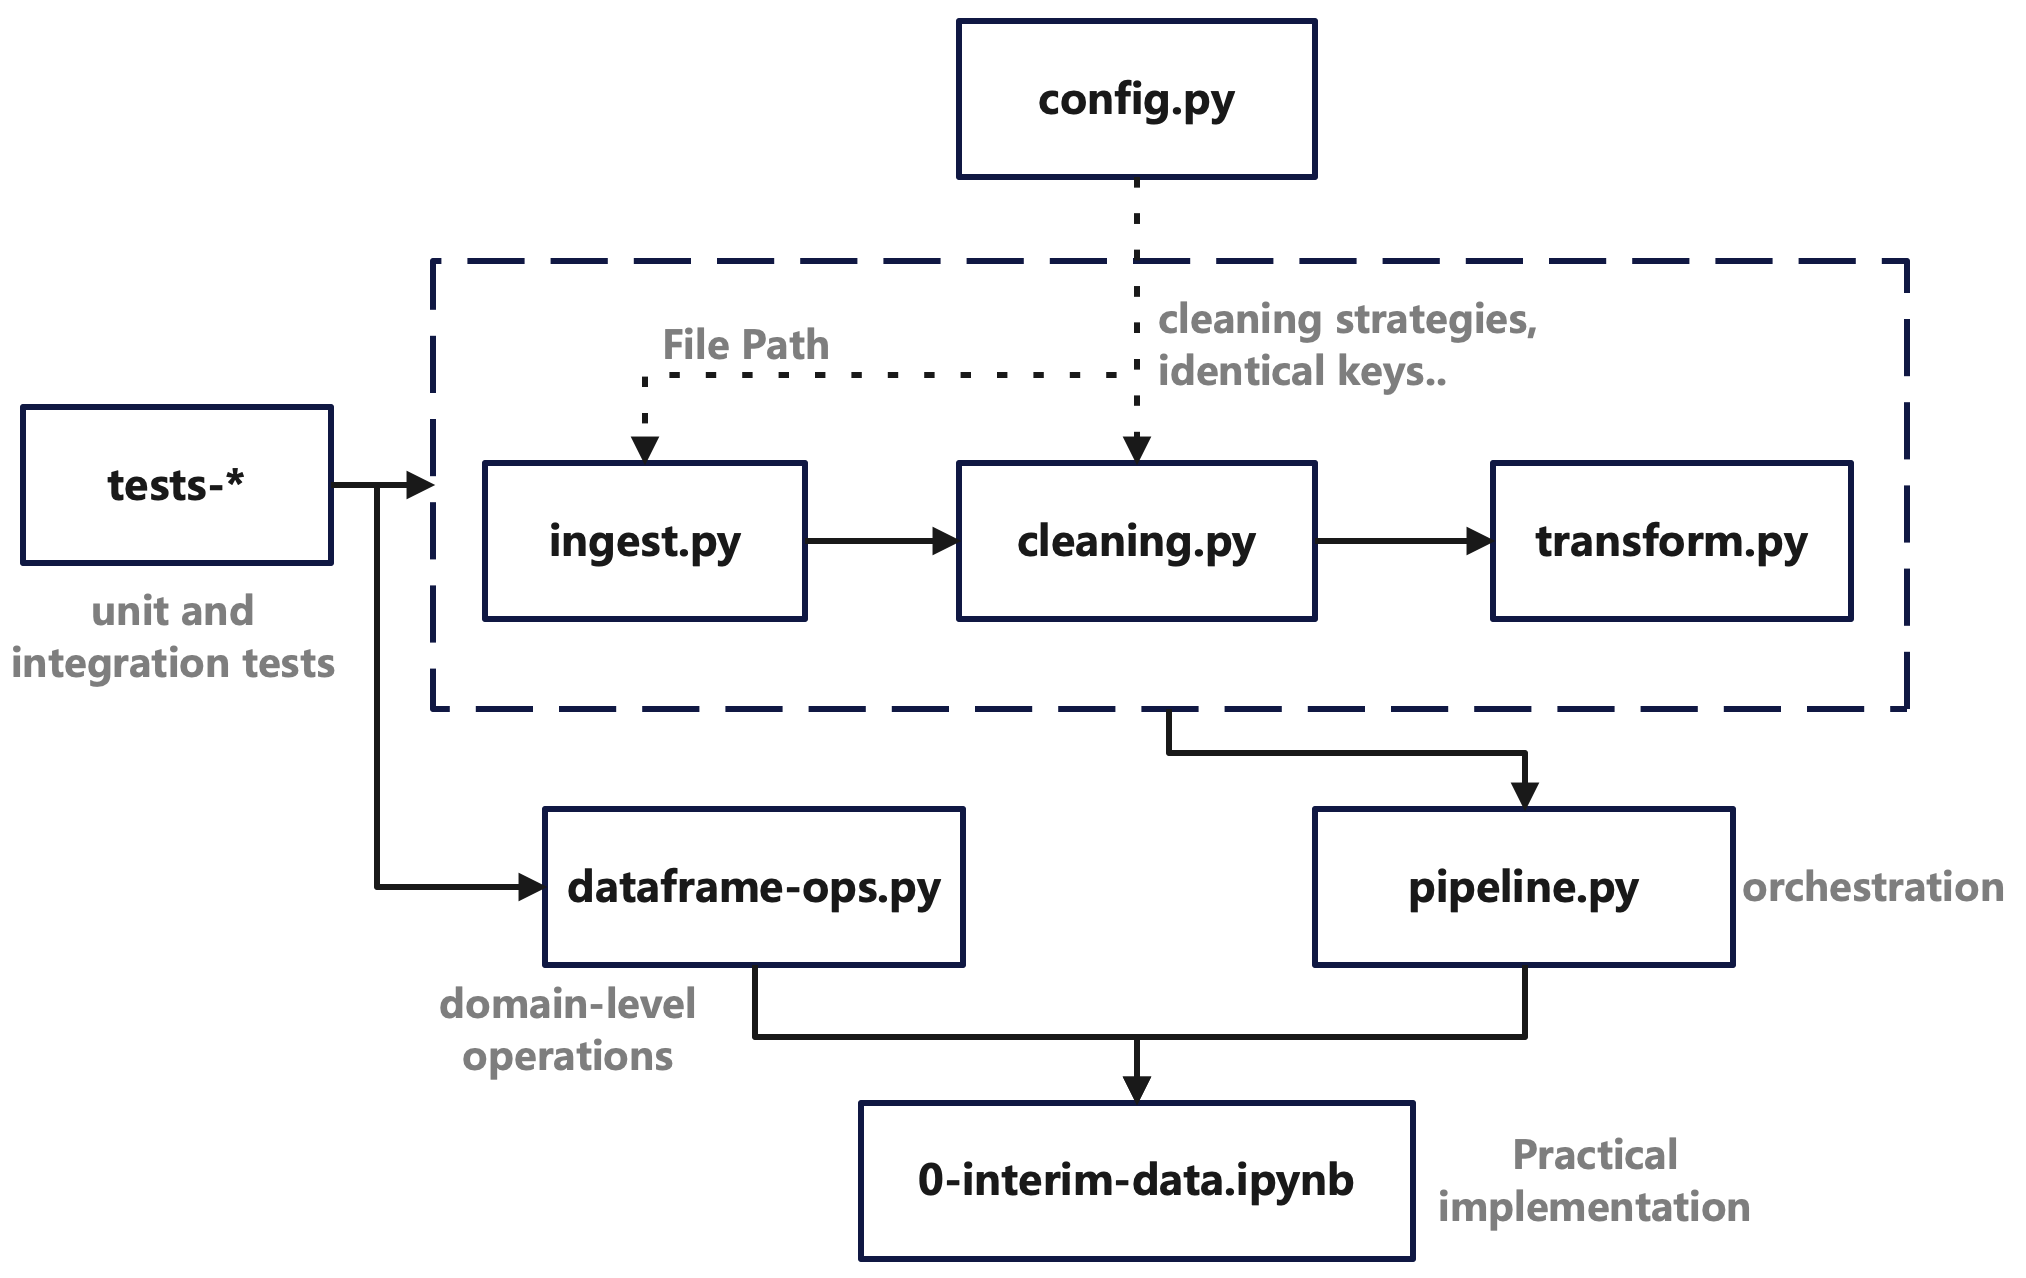
\includegraphics[width=0.9\textwidth]{../results/preliminary_results/implementPlan_example_codebase.png}
    \caption{Demonstration of Workflow for Implementing and Integrating Hellinger Transformation into Complete Data Processing Pipeline}
    \label{fig:implementPlan_example_codebase}
\end{figure}

With this highly integrated modularization, the previously long and complex code can be enclosed in these
separated modules and the application work can be achieved by a few lines of code.
Like the following lines of code in Figure \textcolor{blue}{\ref{fig:example_lightweight_code_completed}} achieve the whole transformation and data merging work
in the Jupyter notebook, which used to require much more extensive and vulnerable code within the same notebook:

\begin{figure}[!h]
    \centering
    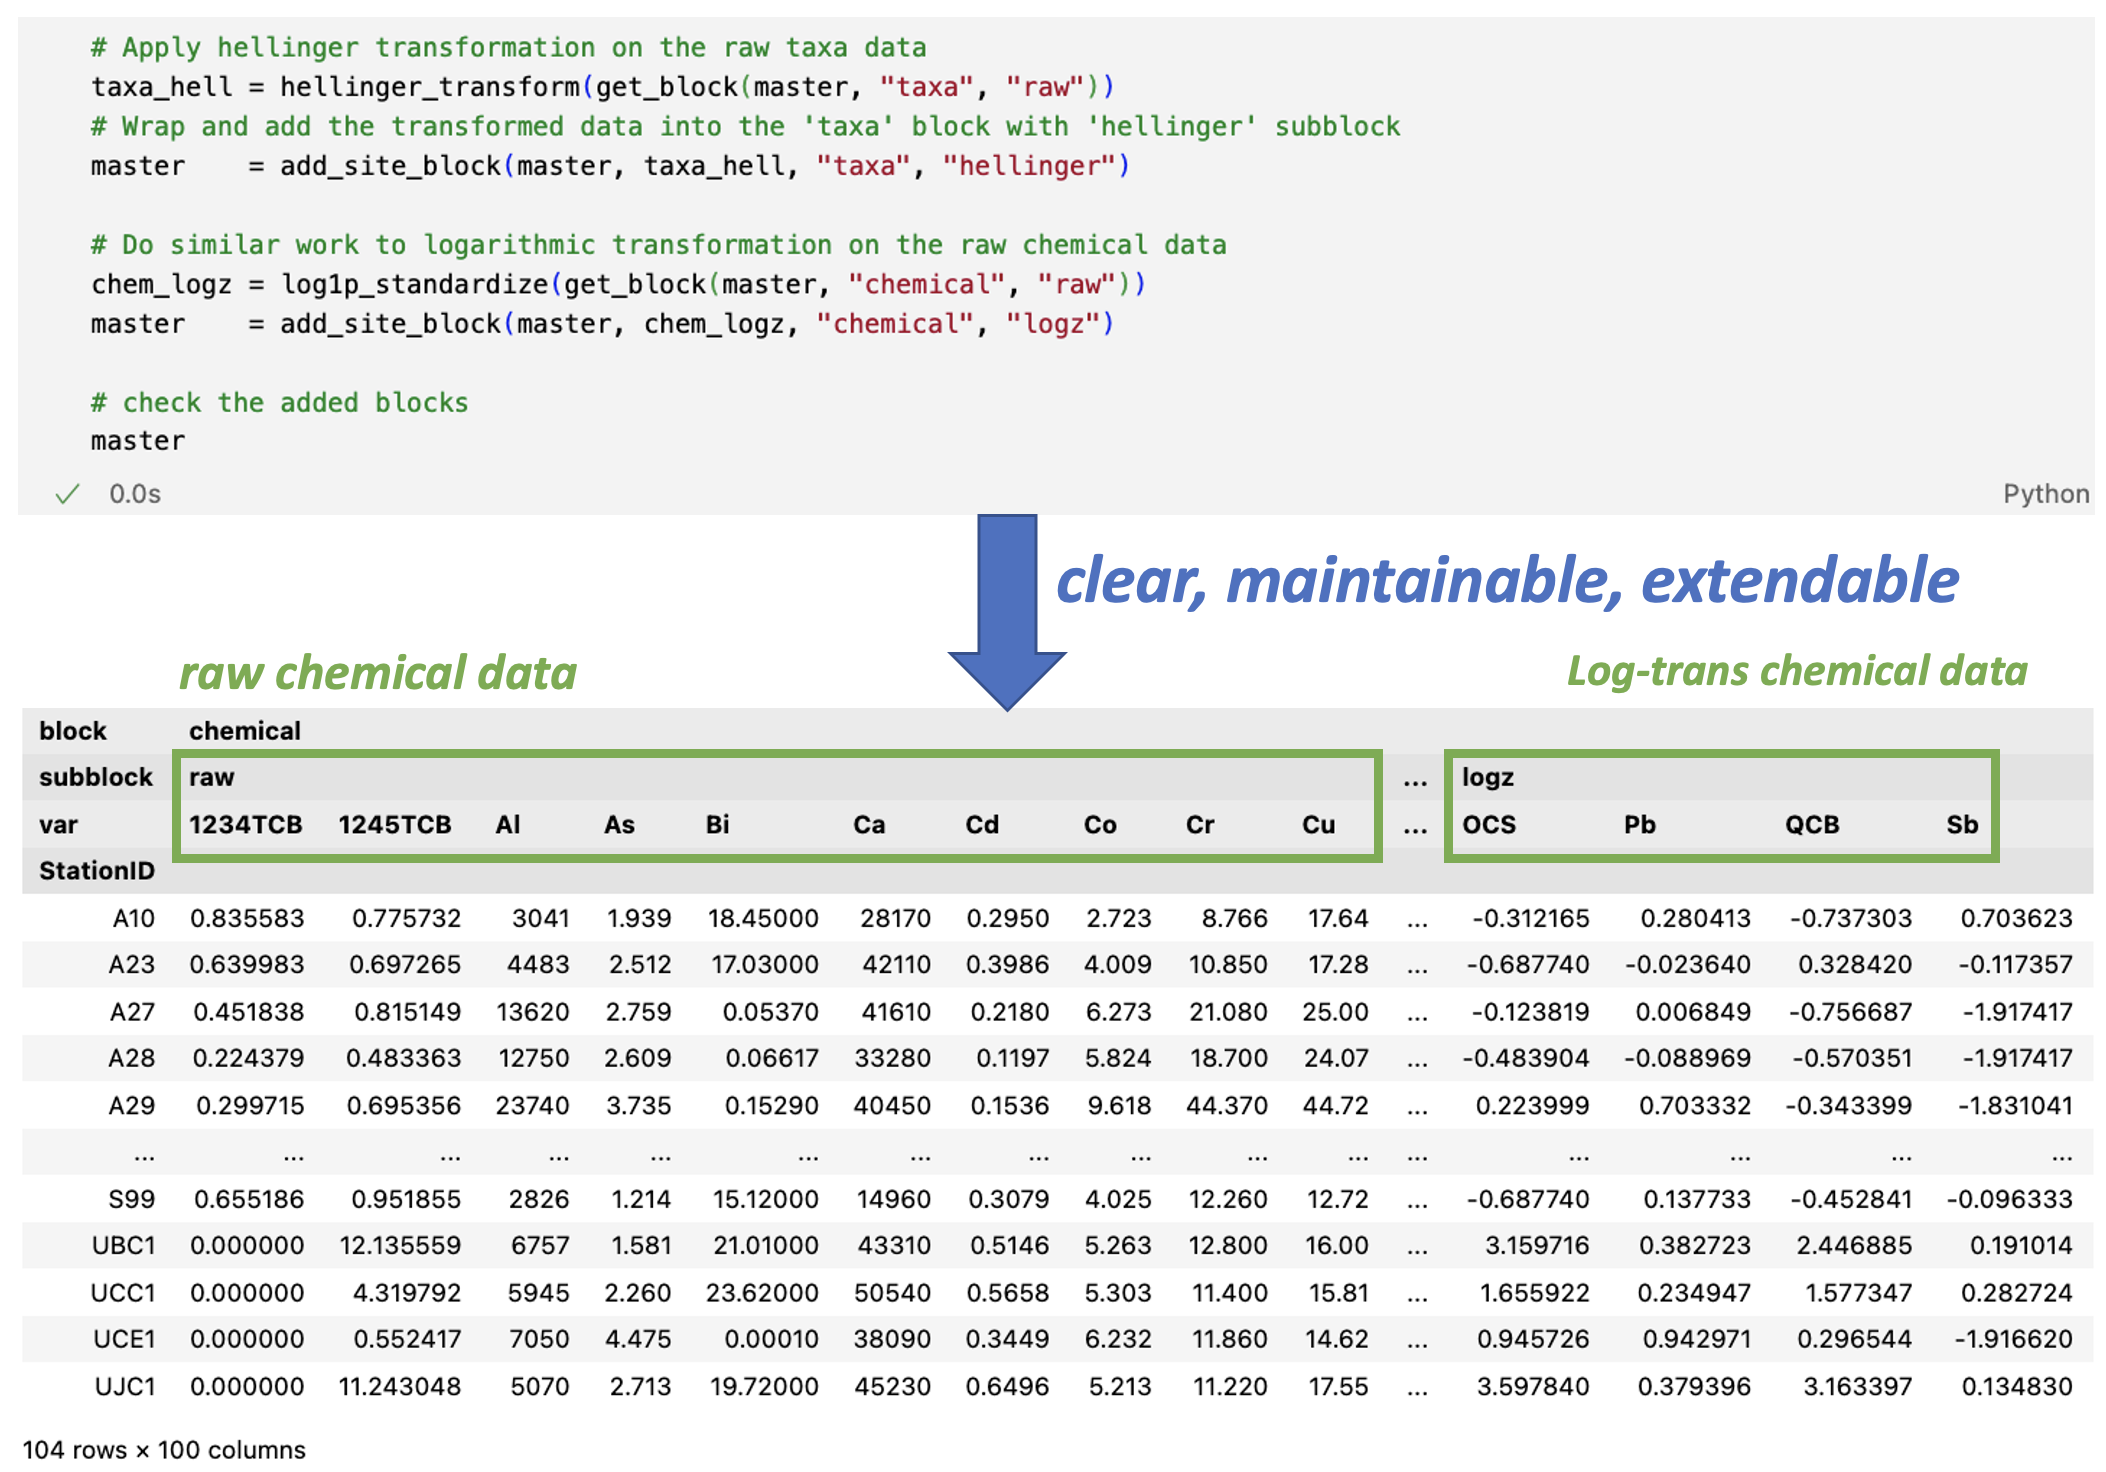
\includegraphics[width=0.9\textwidth]{../results/preliminary_results/example_lightweight_code_completed.png}
    \caption{The lines of code needed to achieve the above discussed operations in practical scenarios and the resulting integrated data frame from the operation}
    \label{fig:example_lightweight_code_completed}
\end{figure}




\subsection{General Project Structure and Rationale}

Generally speaking, the project follows a modular and well-organized structure to support both 
research reproducibility and software engineering best practices.
The folder layout is as follows:

\begin{itemize}
    \item \textbf{configs}: centralizes configuration files (e.g., paths, random seeds, parameter settings), ensuring experiments are reproducible and adjustable without modifying code.
    \item \textbf{data}: stores raw, interim, and processed datasets in a structured hierarchy, making data provenance transparent and simplifying pipeline automation.
    \item \textbf{documents}: contains draft texts, LaTeX notes, and thesis-related writeups, providing a bridge between research outputs and manuscript preparation.
    \item \textbf{figures}: keeps all generated visualizations, plots, and diagrams organized for easy reuse in the thesis and publications.
    \item \textbf{notebooks}: hosts exploratory Jupyter notebooks, which serve as an interface for practical implementation, quick testing, and visualization.
    \item \textbf{reference}: used for bibliographic resources, papers, and supplementary literature, ensuring traceability of scientific background.
    \item \textbf{src}: holds the main source code in a modular format (e.g., \texttt{ingest.py}, \texttt{cleaning.py}, \texttt{pipeline.py}), which separates concerns between ingestion, cleaning, transformation, and higher-level operations.
    \item \textbf{tests}: includes unit tests and validation scripts to ensure correctness and robustness of each module across different scenarios.
    \item \textbf{artifacts}: stores intermediate results, logs, and model checkpoints, preserving computational outcomes for reproducibility and debugging.
    \item \textbf{pyproject.toml}: defines the project environment, dependencies, and metadata, which standardizes reproducibility across systems.
\end{itemize}

\noindent This design provides several benefits:
\begin{enumerate}
    \item \textbf{Reproducibility}: Configurations, raw data, and processed results are explicitly separated, making workflows transparent and repeatable.
    \item \textbf{Scalability}: Modular code in \texttt{src/} and standardized data storage enable extensions (e.g., adding new datasets or models) with minimal disruption.
    \item \textbf{Clarity}: Clear distinction between code, data, results, and documentation reduces confusion and facilitates collaboration or future reuse.
    \item \textbf{Professionalism}: The structure aligns with common practices in industrial data science and academic research, ensuring maintainability and credibility of the project.
\end{enumerate}


\clearpage
\section{Supervisory Dissolution}
	The student agrees that supervision will be dissolved if any of the following happen:
	\begin{itemize}
	\item Two consecutive progress reports are unacceptable
	\item Three consecutive progress reports are concerning/unacceptable
	\item An academic integrity violation is suspected by the supervisor and suspected by at least one other faculty member.
	\end{itemize}
	
\clearpage
\section{Timeline}

\begin{table}[!ht]
\centering
\caption{Thesis Timeline (July 2025 – April 2026)}
\renewcommand{\arraystretch}{1.4}
\begin{tabularx}{\textwidth}{>{\bfseries}l X}
\hline
\textbf{Month} & \textbf{Tasks and Milestones} \\
\hline
\textbf{July 2025} & 
Finalize proposal structure; refine Introduction and Objectives. Read papers on PCA, quantile regression, and CEC. Organize past coding work into reusable modules. \\

\textbf{August 2025} & 
Complete Literature Review section. Start building the prototype bioassessment pipeline using synthetic and real datasets (e.g., Lake Erie). Begin clustering and PCA integration. \\

\textbf{September 2025} & 
Run quantile regression and threshold analysis. Compare models (with and without environmental variables). Begin writing Methods section. \\

\textbf{October 2025} & 
Refine results from PCA + QR analysis. Add validation and comparison between reference vs non-reference site classification. Draft Results section. \\

\textbf{November 2025} & 
Start integrating all sections into a full thesis draft. Revise Introduction and Methods. Begin drafting Discussion and Limitations. \\

\textbf{December 2025} & 
Review thesis draft with supervisors. Incorporate feedback. Conduct final analysis on complementary methods (e.g., environmental clustering, alternative indicators). \\

\textbf{January 2026} & 
Finalize analysis and graphs. Polish Discussion and Conclusions. Prepare supplementary materials (e.g., appendices, raw data logs). \\

\textbf{February 2026} & 
Submit a near-final draft for internal review. Schedule thesis defense. Begin slide and poster preparation for defense or conferences. \\

\textbf{March 2026} & 
Make final revisions based on internal review. Practice oral presentation. Collect forms and approvals. Submit official documents. \\

\textbf{April 2026} & 
Defend thesis. Submit final version. Prepare data archive, GitHub repo, and documentation. Celebrate completion! \\
\hline
\end{tabularx}
\end{table}

\clearpage
\bibliographystyle{plain}  % or use unsrt if you want citations in order of appearance
\bibliography{sections/Reference}   % your .bib file, without .bib extension

\clearpage
\section{Appendix}

\subsection{Tables}

\begin{table}[htbp]
\centering
\caption{Environmental Variables and Their Explanations}
\label{tab:env_variables}
\renewcommand{\arraystretch}{1.3}
\begin{tabular}{|>{\centering\arraybackslash}m{6cm}|>{\centering\arraybackslash}m{8.5cm}|}
\hline
\textbf{Variable Name} & \textbf{Explanation} \\
\hline
Site\_ID & Unique identifier for each sampling site \\
Lake\_or\_River & Indicates whether the site is in a lake or river \\
Latitude & Geographic latitude coordinate \\
Longitude & Geographic longitude coordinate \\
Total\_Organic\_Carbon\_LOI\_percent & Total organic carbon content (loss on ignition, as \%) \\
Water\_Depth\_m & Water depth at the sampling location (meters) \\
Water\_Temperature\_C & Water temperature in degrees Celsius \\
Dissolved\_Oxygen\_Concentration\_mgL & Dissolved oxygen concentration in milligrams per liter \\
Median\_Particle\_Size\_Phi & Median particle size of sediment (Phi scale) \\
\hline
\end{tabular}
\end{table}

\begin{table}[htbp]
\centering
\caption{Taxonomic Variables and Their Explanations}
\label{tab:taxonomic_variables}
\renewcommand{\arraystretch}{1.3}
\begin{tabular}{|>{\centering\arraybackslash}m{4.5cm}|>{\centering\arraybackslash}m{7.5cm}|}
\hline
\textbf{Taxonomic Group} & \textbf{Explanation} \\
\hline
Oligochaeta & Aquatic segmented worms \\
Nematoda & Roundworms \\
Chironomidae & Non-biting midges (larvae) \\
Ceratopogonidae & Biting midges \\
Hexagenia & Mayfly genus (larvae) \\
Caenis & Mayfly genus (larvae) \\
Hydropsychidae & Net-spinning caddisflies \\
Other Trichoptera & Other caddisfly families \\
Amphipoda & Small crustaceans (e.g., scuds) \\
Dreissena & Zebra/quagga mussels \\
Acari & Aquatic mites \\
Hydrozoa & Small predatory animals (hydroids) \\
Hirudinea & Leeches \\
Turbellaria & Flatworms \\
Gastropoda & Snails and slugs \\
Sphaeriidae & Fingernail clams \\
\hline
\end{tabular}
\end{table}

\begin{table}[htbp]
\centering
\caption{Stressors and Their Explanations}
\label{tab:stressors}
\renewcommand{\arraystretch}{1.3}
\begin{tabular}{|>{\centering\arraybackslash}m{3.5cm}|>{\centering\arraybackslash}m{8.5cm}|}
\hline
\textbf{Chemical/Contaminant} & \textbf{Explanation} \\
\hline
Al & Aluminum (trace metal) \\
As & Arsenic (toxic element) \\
Bi & Bismuth (trace element) \\
Ca & Calcium (major element, hardness) \\
Cd & Cadmium (toxic metal) \\
Co & Cobalt (trace element) \\
Cr & Chromium (trace metal) \\
Cu & Copper (trace metal, micronutrient) \\
Fe & Iron (major element, micronutrient) \\
Hg & Mercury (highly toxic metal) \\
K & Potassium (major element) \\
Mg & Magnesium (major element, hardness) \\
Mn & Manganese (trace element) \\
Na & Sodium (major element) \\
Ni & Nickel (trace metal) \\
Pb & Lead (toxic metal) \\
Sb & Antimony (trace element) \\
V & Vanadium (trace element) \\
Zn & Zinc (trace metal, micronutrient) \\
\%OC & Percent organic carbon \\
1245-TCB & 1,2,4,5-Tetrachlorobenzene (organic pollutant) \\
1234-TCB & 1,2,3,4-Tetrachlorobenzene (organic pollutant) \\
QCB & Quintachlorobenzene (organic pollutant) \\
HCB & Hexachlorobenzene (organic pollutant) \\
OCS & Octachlorostyrene (organic pollutant) \\
p,p'-DDE & DDT breakdown product \\
p,p'-DDD & DDT breakdown product \\
mirex & Organochlorine insecticide \\
Heptachlor Epoxide & Organochlorine pesticide breakdown product \\
total PCB & Total polychlorinated biphenyls \\
\hline
\end{tabular}
\end{table}

\begin{table}[htbp]
\centering
\caption{Explanation, Habitat, and Survival Rate in Fast/Slow Water for Each Taxon}
\begin{tabular}{|c|c|c|c|}
\hline
\textbf{Taxa} & \textbf{Explanation} & \textbf{Habitat Type} & \textbf{Survival Rate (Fast/Slow Water)} \\
\hline
Oligochaeta & Aquatic segmented worms & Both (lentic/lotic) & Moderate/High \\
Nematoda & Roundworms & Both (lentic/lotic) & Moderate/High \\
Chironomidae & Non-biting midge larvae & Both (lentic/lotic) & Moderate/High \\
Ceratopogonidae & Biting midge larvae & Both (lentic/lotic) & Moderate/Moderate \\
Hexagenia & Burrowing mayflies & Lentic (lakes/ponds) & Low/High \\
Caenis & Small mayflies & Both (lentic/lotic) & Low/Moderate \\
Hydropsychidae & Net-spinning caddisflies & Lotic (streams/rivers) & High/Low \\
Other Trichoptera & Other caddisflies & Both (lentic/lotic) & Moderate/Moderate \\
Amphipoda & Small crustaceans & Both (lentic/lotic) & Moderate/High \\
Dreissena & Zebra/quagga mussels & Lentic, large rivers & Low/High \\
Acari & Aquatic mites & Both (lentic/lotic) & Moderate/High \\
Hydrozoa & Predatory invertebrates & Lentic (lakes/ponds) & Low/High \\
Hirudinea & Leeches & Both (lentic/lotic) & Low/High \\
Turbellaria & Flatworms & Both (lentic/lotic) & Low/High \\
Gastropoda & Aquatic snails & Both (lentic/lotic) & Low/High \\
Sphaeriidae & Fingernail clams & Both (lentic/lotic) & Low/High \\
\hline
\end{tabular}
\end{table}


% statistical description for the chemical data within reference, intermediate, and degraded sites based on PCA assessment
\begin{table}[ht]
\centering
\caption{Chemical Descriptive Statistics by Site Label}
\label{tab:chem_desc}
\begin{tabular}{>{\centering\arraybackslash}m{2.5cm} >{\centering\arraybackslash}m{1.5cm} >{\centering\arraybackslash}m{2cm} >{\centering\arraybackslash}m{2cm} >{\centering\arraybackslash}m{2cm}}
\toprule
 & \textbf{SumReal} & \textbf{degraded} & \textbf{intermediate} & \textbf{reference} \\
\midrule
\multirow[t]{2}{*}{Al} & mean & 4276.423 & 6380.140 & 4319.381 \\
 & std & 2888.769 & 5523.949 & 1767.861 \\
\cline{1-5}
\multirow[t]{2}{*}{As} & mean & 2.186 & 1.777 & 2.232 \\
 & std & 1.602 & 1.290 & 1.041 \\
\cline{1-5}
\multirow[t]{2}{*}{Bi} & mean & 17.085 & 17.505 & 17.622 \\
 & std & 10.352 & 10.273 & 9.722 \\
\cline{1-5}
\multirow[t]{2}{*}{Ca} & mean & 28180.500 & 33518.930 & 28480.714 \\
 & std & 14031.433 & 11400.266 & 11870.107 \\
\cline{1-5}
\multirow[t]{2}{*}{Cd} & mean & 0.535 & 0.351 & 0.271 \\
 & std & 0.649 & 0.202 & 0.233 \\
\cline{1-5}
\multirow[t]{2}{*}{Co} & mean & 4.049 & 4.497 & 3.984 \\
 & std & 1.733 & 2.209 & 1.118 \\
\cline{1-5}
\multirow[t]{2}{*}{Cr} & mean & 13.254 & 12.830 & 9.007 \\
 & std & 16.373 & 11.835 & 2.937 \\
\cline{1-5}
\multirow[t]{2}{*}{Cu} & mean & 16.958 & 18.082 & 12.946 \\
 & std & 22.388 & 29.120 & 9.003 \\
\cline{1-5}
\multirow[t]{2}{*}{Fe} & mean & 9495.000 & 11246.789 & 9650.905 \\
 & std & 5392.824 & 6804.654 & 3856.739 \\
\cline{1-5}
\multirow[t]{2}{*}{Hg} & mean & 0.474 & 0.324 & 0.196 \\
 & std & 1.230 & 0.420 & 0.365 \\
\cline{1-5}
\multirow[t]{2}{*}{K} & mean & 818.927 & 1285.558 & 845.657 \\
 & std & 638.053 & 1092.550 & 411.332 \\
\cline{1-5}
\multirow[t]{2}{*}{Mg} & mean & 12849.500 & 15204.175 & 12269.143 \\
 & std & 6104.202 & 5764.037 & 5281.794 \\
\cline{1-5}
\multirow[t]{2}{*}{Mn} & mean & 161.228 & 188.900 & 161.905 \\
 & std & 76.973 & 86.663 & 57.883 \\
\cline{1-5}
\multirow[t]{2}{*}{Na} & mean & 118.998 & 134.042 & 123.611 \\
 & std & 49.081 & 43.693 & 41.021 \\
\cline{1-5}
\multirow[t]{2}{*}{Ni} & mean & 11.225 & 12.399 & 9.136 \\
 & std & 8.851 & 8.424 & 3.542 \\
\cline{1-5}
\multirow[t]{2}{*}{Pb} & mean & 12.515 & 8.774 & 8.573 \\
 & std & 32.312 & 22.204 & 18.750 \\
\cline{1-5}
\multirow[t]{2}{*}{Sb} & mean & 17.262 & 16.765 & 18.001 \\
 & std & 11.879 & 13.115 & 13.743 \\
\cline{1-5}
\multirow[t]{2}{*}{V} & mean & 15.274 & 18.353 & 15.183 \\
 & std & 7.012 & 9.560 & 4.408 \\
\cline{1-5}
\multirow[t]{2}{*}{Zn} & mean & 52.732 & 46.181 & 35.677 \\
 & std & 48.896 & 44.586 & 17.938 \\
\cline{1-5}
\multirow[t]{2}{*}{\%OC} & mean & 2.110 & 2.405 & 1.779 \\
 & std & 1.599 & 1.458 & 0.682 \\
\cline{1-5}
\multirow[t]{2}{*}{1245-TCB} & mean & 0.906 & 1.201 & 0.555 \\
 & std & 2.321 & 2.143 & 1.035 \\
\cline{1-5}
\multirow[t]{2}{*}{1234-TCB} & mean & 0.252 & 0.234 & 0.253 \\
 & std & 0.257 & 0.240 & 0.332 \\
\cline{1-5}
\multirow[t]{2}{*}{QCB} & mean & 0.729 & 1.255 & 0.636 \\
 & std & 1.015 & 3.055 & 0.871 \\
\cline{1-5}
\multirow[t]{2}{*}{HCB} & mean & 2.759 & 17.713 & 2.904 \\
 & std & 4.291 & 83.487 & 6.011 \\
\cline{1-5}
\multirow[t]{2}{*}{OCS} & mean & 1.213 & 1.502 & 0.721 \\
 & std & 3.395 & 3.606 & 1.874 \\
\cline{1-5}
\multirow[t]{2}{*}{p,p'-DDE} & mean & 0.679 & 0.485 & 0.324 \\
 & std & 1.255 & 0.930 & 0.328 \\
\cline{1-5}
\multirow[t]{2}{*}{p,p'-DDD} & mean & 3.879 & 0.772 & 0.862 \\
 & std & 14.634 & 1.039 & 0.923 \\
\cline{1-5}
\multirow[t]{2}{*}{mirex} & mean & 0.253 & 0.212 & 0.134 \\
 & std & 0.682 & 0.332 & 0.242 \\
\cline{1-5}
\multirow[t]{2}{*}{Heptachlor Epoxide} & mean & 0.098 & 0.051 & 0.071 \\
 & std & 0.235 & 0.250 & 0.211 \\
\cline{1-5}
\multirow[t]{2}{*}{total PCB} & mean & 15.137 & 10.705 & 7.715 \\
 & std & 32.189 & 36.285 & 16.795 \\
\cline{1-5}
\bottomrule
\end{tabular}
\end{table}

\subsection{Index-based methods for quantitative stress metrics}
\begin{tcolorbox}[colback=yellow!10!white,
                                        colframe=blue!80!black,
                                        title = Introduce the index-based methods for quantitative stress metrics,
                                        fonttitle=\bfseries] 

PCA is mainly for exploratory work, like finding patterns, associations in the data.
It may be used to score the sediment contamination level, but only comparing relative abundance 
of stressor elements among the sites, lacking a little standards to accurately assess the contamination level.

Index-based methods can be used to quantitatively assess the sediment contamination level.
Such method needs more empirical and theoretical support than PCA, but it offers a more standardized way
to assess the contamination level, which is theoretically more accurate.

\textbf{Combining the PCA and index-based methods} is a good idea to explore the sediment contamination level.
I am thinking about what do they mean in contamination assessment, and how to combine them with
a reasonable logical flow.

\end{tcolorbox}

\subsection{Principal Component Analysis based methods to explore contaminant association and patterns }

\textcolor{blue}{Discuss the reason why and how PCA can be used to assess the sediment contamination level and reflect the 
aquatic ecological integrity.}

In SVD, a data matrix $X$ is decomposed as $X = U \Sigma V^T$, where $U$ and $V$ are orthogonal matrices and
 $\Sigma$ is a diagonal matrix of singular values.
For PCA, the principal components correspond to
the directions of maximum variance, which are given by the right singular vectors in $V$.
By incorporating weights into the data matrix, Weighted PCA modifies the SVD process 
to emphasize certain observations(row or column), allowing for more flexible dimensionality reduction 
tailored to the importance of each data point.

Given a data matrix $X \in \mathbb{R}^{m \times n}$, the SVD decomposes $X$ as $X = U \Sigma V^T$, where:
\begin{itemize}
    \item $U \in \mathbb{R}^{m \times m}$ contains the left singular vectors (columns),
    \item $\Sigma \in \mathbb{R}^{m \times n}$ is a diagonal matrix of singular values,
    \item $V \in \mathbb{R}^{n \times n}$ contains the right singular vectors (columns).
\end{itemize}

To solve for $U$ and $V$:
\begin{enumerate}
    \item Compute $X^T X$ and find its eigenvectors and eigenvalues. The eigenvectors form the columns of $V$.
    \item It can be proven that \(\mu_i^T = \frac{X v_i}{\sigma_i}\) is the $i$-th column of $U$, where $\sigma_i$ is the $i$-th singular value(square root of eigenvalue \(\lambda_i\)).
    \item The singular values in $\Sigma$ are the square roots of the nonzero eigenvalues from either $X X^T$ or $X^T X$.
\end{enumerate}

Mathematically, given a matrix $X$ of shape $(m, n)$, the SVD can be expressed as: 
\[
(X^T X) V = V \Lambda, \quad \Lambda = \text{diag}(\lambda_1, \lambda_2, \ldots, \lambda_n)
\]
According to spectral theorem, the eigenvalues $\lambda_i$ are non-negative and can be ordered as $\lambda_1 \geq \lambda_2 \geq \ldots \geq \lambda_n \geq 0$.
\(V\) is an orthogonal matrix, meaning \(V^T V = I\), where \(I\) is the identity matrix.
It gives:
\[
(X^T X) = V \Lambda V^T
\]
To a centered sample matrix of size \(m\) with \(n\) features, its covariance matrix is \(\frac{1}{m-1} (X^T X)\).
Via the eigenvalue decomposition, the variation in it can be expressed by the paris of eigenvalues and eigenvectors,
which are a series of rank-one matrices that carry different and independent information:
\[
\frac{1}{m-1} (X^T X) = \frac{1}{m-1} \sum_{i=1}^{n} \lambda_i v_i v_i^T
\]

Therefore, when columns in \(X\) represent different features, the columns \(v_i\) of \(V\) are the principal components 
that have its values as the linear combinations of the original features, and the scaled eigenvalues \(\frac{\lambda_i}{m-1}\)
as the amount of variation explained by each principal component.

Weighted PCA leverages the Singular Value Decomposition (SVD)
to extract principal components from weighted data.

\textcolor{blue}{Preparing to explain why this ordinal decomposition is not good for our case, and how we can 
improve it by considering the weights for different chemical elements and filtering out the from the PCs}

\subsection{Hierarchical Clusering analysis for Zoobenthic Communicty Indicator Construction}

Application of Hierarchical Clustering in Stressor-Community Analysis
Overview
Hierarchical clustering offers a data-driven approach to group sampling sites based on environmental or 
community-level similarities. Unlike partitioning methods, hierarchical clustering builds a nested tree
(dendrogram) that captures the progressive grouping of observations based on their dissimilarities.
In the context of my program, hierarchical clustering can be leveraged to define natural environmental 
classes prior to modeling the biological response to stressors.

Let each observation \( x_i \in \mathbb{R}^p \) denote a site with p-dimensional attributes (e.g., environmental variables). 
The dissimilarity between two observations \( x_i \) and \( x_{i'} \) is measured by a distance function,
often chosen as the squared Euclidean distance:
\[ d(x_i, x_{i'}) = \sum_{j=1}^p (x_{ij} - x_{i'j})^2 \]

Based on the distance metric, we can define the similarity measure on variable and observation levels as the following:
\[
\begin{aligned}
    &\text{Variable level:} \quad d_j(x_{ij}, x_{i'j}) = (x_{ij} - x_{i'j})^2, \quad j = 1, \ldots, p \\
    &\text{Observation level:} \quad d(x_i, x_{i'}) = \sum_{j=1}^{p} (x_{ij} - x_{i'j})^2 \\
\end{aligned}
\]

To cluster level \( D_C \), we can define other alternatives to the dissimilarity measures, commonly including:

\[ D_{SL}(G, H) = \min_{i \in G,\; i' \in H} d(x_i, x_{i'}) \quad \text{(Single Linkage)} \]
\[ D_{CL}(G, H) = \max_{i \in G,\; i' \in H} d(x_i, x_{i'}) \quad \text{(Complete Linkage)} \]
\[ D_{GA}(G, H) = \frac{1}{|G||H|} \sum_{i \in G} \sum_{i' \in H} d(x_i, x_{i'}) \quad \text{(Average Linkage)} \] 

\begin{itemize}
    \item \textbf{Use in the Program:}
    \begin{itemize}
        \item Hierarchical clustering is used to categorize sampling sites into clusters with similar environmental conditions before building predictive models linking taxonomic composition to stressor levels.
        \item This enables a two-stage analysis:
        \begin{itemize}
            \item Use environmental variables to form environmental clusters (reference site classification).
            \item Model stressor-community relationships within or across these clusters to control for natural variation.
        \end{itemize}
    \end{itemize}
    \item \textbf{Advantages:}
    \begin{itemize}
        \item Does not require pre-specification of the number of clusters.
        \item Produces a dendrogram showing how clusters are formed step-by-step.
        \item Enables ecological interpretation of clusters through tree visualization.
        \item Allows separation of natural variation from anthropogenic stress impacts.
    \end{itemize}
    \item \textbf{Model-Based Interpretation:}
    \begin{itemize}
        \item Assume that each cluster \( k \) corresponds to a latent distribution \( p_k(x) \), with the overall mixture model:
        \[
        p(x) = \sum_{k=1}^K \pi_k p_k(x)
        \]
        \item Each observation is generated as \( x \sim p_k(x) \) conditional on cluster membership \( k \), providing a statistical grounding for hierarchical clustering in unsupervised structure discovery.
    \end{itemize}
\end{itemize}


\textcolor{blue}{waiting to add more specific details after applying the clustering on the data and getting
some preliminary results.}

% \textcolor{blue}{Discuss why Clustering analysis is needed and how it was conducted
% on the taxonomic composition data to group them into clusters of different environmental conditions.}

% It needs to explain why directly clustering on the taxonomic composition can group them 
% into clusters of different environmental conditions instead of contamination levels.
% Because the assumption is: taxonomic compostion reponds to both the environmental conditions and 
% the contamination levels. If we think the clustering results are domainated by the environmental 
% conditions, that implies the influence by environment is stronger than by the contamination levels.


% \textcolor{blue}{These sites within each clusters should stay in specific environmental conditions.}

% Hierarchical clustering is a method of cluster analysis that seeks to build a hierarchy of clusters,
% it supports users to choose the number of clusters by cutting the dendrogram at a desired level, and 
% the testing on how well the clustering results represent the data structure is also available.




\subsection{Piecewise Quantile Regression for Threshold Determination}

% \textcolor{blue}{Discuss why PQRM is better than common linear regression in detecting 
% potential thresholds}

Let $m_\tau(x; \boldsymbol{\beta}_\tau, \boldsymbol{\alpha}_\tau)$ be the $\tau$th quantile of the conditional distribution 
of the ecological response given environmental condition. Then we define:

\[
y_\tau = m_\tau(x; \boldsymbol{\beta}_\tau, \boldsymbol{\alpha}_\tau) + \varepsilon_\tau.
\]

The form is similar to the linear regression model, but there are no restrictions on the distribution of error term $\varepsilon_\tau$, 
which means the error terms can be heteroscedastic(non-constant variance).


Then the \textbf{PQRM} with two breakpoints is defined as:

\[
m_\tau(x_i; \boldsymbol{\beta}_\tau, \boldsymbol{\alpha}_\tau) =
\begin{cases}
\beta_{0\tau} + \beta_{1\tau} x_i & \text{for } x_i \leq \alpha_{1\tau} \\
\beta_{0\tau} + \beta_{1\tau} x_i + \beta_{2\tau}(x_i - \alpha_{1\tau}) & \text{for } \alpha_{1\tau} < x_i \leq \alpha_{2\tau} \\
\beta_{0\tau} + \beta_{1\tau} x_i + \beta_{2\tau}(x_i - \alpha_{1\tau}) + \beta_{3\tau}(x_i - \alpha_{2\tau}) & \text{for } x_i > \alpha_{2\tau}
\end{cases}
\tag{3}
\]

The \(\tau\) subscript indicates the quantile level.
Breakpoints are spotted in the predictor space, which seems uncorrelated with the response variable and its quantile,
but they are not fixed and should be estimated under different quantile levels so that
the piecewise model provides a better performance on the data with such quantile level.
That is, the breakpoints are also functions of the quantile level \(\tau\).
\[
Y_{\tau} = X(\alpha_{_({\tau}; 1)}, \alpha_{_({\tau}; 2)}) \cdot \boldsymbol{\beta_{\tau}} + \boldsymbol{\varepsilon_{\tau}}
\]

Because the model are not predicting the means but the quantiles of $y$'s at given $x$'s,
the measurement for the model performance should no longer be the mean squared error(MSE),
\footnote{If a model regresses the mean of $Y$, it should outperform other models in the measurement of MSE, assuming the assumptions are satisfied.}
the check function is the loss function, which is defined as:
\[
\rho_\tau(u) =
\begin{cases}
\tau u & \text{if } u \geq 0 \\
(\tau - 1) u & \text{if } u < 0
\end{cases}
\quad \text{where } u = y - \hat{y}
\]

The loss function is a random variable that derivatives from $Y$, and it also can be viewed as a function of 
the prediction $\hat{y_{\tau}}$, which is not a RV.
A specific quantile can be found by minimizing the expected loss function - $E({\rho_{\tau}(Y - \hat y_{\tau})})$ with respect to $\hat y_{\tau}$ across
the observations:
\[
    {\displaystyle q_{Y}(\tau )={\underset {\hat y_{\tau}}{\mbox{arg min}}}E(\rho _{\tau }(Y-\hat y_{\tau}))={\underset {\hat y_{\tau}}{\mbox{arg min}}}{\biggl \{}(\tau -1)\int _{-\infty }^{\hat y_{\tau}}(y-\hat y_{\tau})dF_{Y}(y)+\tau \int _{\hat y_{\tau}}^{\infty }(y-\hat y_{\tau})dF_{Y}(y){\biggr \}}} 
\]

The expectation is no more a random variable, but a function of $(\hat y_{\tau}, y, F_Y(y))$.
By computing the derivative of it with respect to $\hat y_{\tau}$, the equation is determined by $(\hat y_{\tau}, F_Y(y))$.
Settting it to zero and letting $q_{\tau}$ the solution of $\hat y_{\tau}$ to the equation, we have:

\[
    {\displaystyle 0=(1-\tau )\int _{-\infty }^{q_{\tau }}dF_{Y}(y)-\tau \int _{q_{\tau }}^{\infty }dF_{Y}(y).} 
\]

It gives:
\[
F_Y(q_{\tau}) = \tau
\]

Therefore, $\rho_\tau(u)$ is a valid loss function for inferring the quantile of $Y$.
However, when building quantile regression on $Y$ with $X$, we need to have enough observations on each condition of $X$.
Becasue there is no assumption that residuals are homoscedastic, the globally minimized loss function does not necessarily 
bring good predictions on all conditions, which is different to the linear regression model.

To a given condition $x$, the quantile of $\tilde y$ is defined as:
\[
    {\displaystyle q_{\tilde y|x}(\tau )={\underset {\hat y_{\tau}}{\mbox{arg min}}}E(\rho _{\tau }(\tilde y - \hat y_{\tau})|X)={\underset {\hat y_{\tau}}{\mbox{arg min}}}{\biggl \{}(\tau -1)\int _{-\infty }^{\hat y_{\tau}}(y - \hat y_{\tau})dF_{\tilde y|x}(y)+\tau \int _{\hat y_{\tau}}^{\infty }(y-\hat y_{\tau})dF_{\tilde y|x}(y){\biggr \}}} 
\]

The expected loss function that provides quantiles over all observations is:
\[
    E(\rho_{\tau}(\tilde y - \hat y_{\tau})) = \frac{1}{n} \sum_{i=1}^n \rho_\tau(\tilde y_i - x_i^\top \beta_{\tau})
\]

Optimizing it to minimum with respect to $\beta_{\tau}$ gives the optimal $\beta_{\tau}$
\footnote{There should be an assumption of linear relation on the amount changing between $x$ and $\tau$ quantile of $y$, and $\beta$ is the coefficient of that relation.}:
\[
\hat{\beta}\tau = {\underset {\beta_{\tau}}{\mbox{arg min}}} E(\rho_{\tau}(\tilde y - \hat y_{\tau}))
\]



When given two breakpoints, the $(\alpha_{(\tau; 1)}, \alpha_{(\tau; 2)})$ can be iteratively searched by 
Newton-Raphson method. Within each iteration, the loss function is minimized to find the optimal $\beta_{(\tau)}$ vector.

\textcolor{blue}{waiting to add more specific details after applying the clustering on the data and getting
some preliminary results.}


\subsection{Synthetic Data Generation}

Synthetic data generation refers to the process of artificially creating data that mimics 
the statistical properties and structure of real-world datasets. 
The core motivation is to generate data when real data are limited, imbalanced,
 private, or costly to obtain. Synthetic data are widely used in machine learning,
  data privacy preservation, and simulation-based research.

This approach can simulate various data types, 
including tabular (structured), image, text, and time series data. 
The generated data should reflect similar distributions, correlations,
 and interactions as the original data while maintaining flexibility and scalability.

Synthetic data generation can play a supportive role in this study by addressing several data-related challenges 
commonly encountered in ecological assessments:

\begin{itemize}
    \item \textbf{Enhancing model robustness}: By generating additional synthetic observations that mimic the real data structure, we can augment the existing data pool, which helps reduce model overfitting and improve generalization when predicting stressor impacts across unsampled sites.
    
    \item \textbf{Balancing site distribution across gradients}: Many ecological datasets are imbalanced with respect to environmental gradients or stressor intensity levels. Synthetic data can help balance the representation of different ecological zones or stressor conditions, ensuring the model learns from a more evenly distributed set of scenarios.
    
    \item \textbf{Supporting rare condition modeling}: Stressor levels or taxa responses in extreme or under-sampled regions (e.g., highly degraded or pristine sites) can be underrepresented. Synthetic data can simulate these rare cases to aid in threshold detection or to inform prediction in sparsely observed domains.
    
    \item \textbf{Facilitating model testing and validation}: Controlled synthetic datasets can be used to evaluate the behavior and sensitivity of the modeling framework under different stressor-environment-taxa scenarios, helping identify model biases or limits.
    
    \item \textbf{Exploring uncertainty and variability}: Synthetic data allow the introduction of controlled noise and variability, which is useful for evaluating how robust the model is to observational or measurement uncertainty.
\end{itemize}

A simple yet effective approach to synthetic data generation is random sampling (bootstrapping) from the observed dataset.
 Given a dataset \( \mathcal{D} = \{x_1, \dots, x_N\} \), where \( x_i \in \mathbb{R}^p \), 
 synthetic samples are generated by sampling with replacement:
\[
x_i^* \sim \hat{F}, \quad i = 1, \dots, N^*
\]
where \( \hat{F} \) is the empirical distribution of \( \mathcal{D} \), and \( N^* \) is
 the desired number of synthetic samples.

This method preserves the multivariate structure by sampling entire rows, maintaining correlation between features.
 It is non-parametric and computationally efficient.

\textbf{Use in this project:} Random sampling can augment small or imbalanced training sets, support bootstrapped 
threshold estimation, and improve model robustness across environmental gradients.

More common methods for synthetic data generation are summarized in Table \ref{tab:synthetic_data_methods}.

\begin{table}[!h]
\centering
\caption{Summary of common synthetic data generation methods and their applications.}
\label{tab:synthetic_data_methods}
\renewcommand{\arraystretch}{1.3}
\small
\begin{tabular}{|>{\centering\arraybackslash}p{3.5cm}|>{\centering\arraybackslash}p{7cm}|>{\centering\arraybackslash}p{4.2cm}|}
\hline
\textbf{Method} & \textbf{Description} & \textbf{Example Use Case} \\
\hline
\textbf{Random Sampling} & Generate synthetic data by sampling from known statistical distributions (e.g., normal, uniform, Poisson) & Simulating sensor readings or generating test input data \\
\hline
\textbf{SMOTE (Synthetic Minority Oversampling Technique)} & Generates new instances of the minority class by interpolating between existing instances & Addressing class imbalance in classification problems \\
\hline
\textbf{GANs (Generative Adversarial Networks)} & Uses a generator and a discriminator to iteratively create highly realistic synthetic data that mimics the real distribution & Synthetic images, medical data, or tabular data with complex dependencies \\
\hline
\textbf{VAEs (Variational Autoencoders)} & Learns a probabilistic latent space from real data and generates synthetic samples by decoding random samples from that space & Generating synthetic patient records or anomaly detection \\
\hline
\textbf{Agent-based Simulations} & Models behavior of individuals or agents and their interactions to generate data over time & Simulating traffic systems or disease spread \\
\hline
\textbf{Rule-based Generation} & Applies predefined rules and logical templates to construct synthetic data & Automated form testing, fake transactions for system validation \\
\hline
\end{tabular}
\end{table}

\textcolor{blue}{waiting to add more specific details after applying the clustering on the data and getting
some preliminary results.}


\end{document}

